\newpage
{\bfseries МРНТИ 20.20.20}

{\bfseries ПАРАМЕТРИЧЕСКАЯ УСТОЙЧИВОСТЬ БЕСПИЛОТНОГО ЛЕТАТЕЛЬНОГО АППАРАТА}

{\bfseries \textsuperscript{1}А.Т. Мазакова,
\textsuperscript{1}Ш.А.Джомартова, \textsuperscript{1,2}Т.Ж.
Мазаков\textsuperscript{🖂}, \textsuperscript{3}Тойкенов Г.Ч.,}

{\bfseries \textsuperscript{2}М.С. Алиаскар}

\textsuperscript{1}Казахский национальный университет имени аль-Фараби,
Алматы, Казахстан,

\textsuperscript{2}Международный инженерно-технологический университет,
Алматы, Казахстан,

\textsuperscript{3}Казахский национальный женский педагогический
университет, Алматы, Казахстан

{\bfseries \textsuperscript{🖂}}Корреспондент-автор: tmazakov@mail.ru

Цель данной работы заключается в создании алгоритмов и программного
обеспечения для автоматизированной проверки условий устойчивости
динамики беспилотного летательного аппарата, чья математическая модель
представлена системой обыкновенных дифференциальных уравнений. С помощью
системы аналитических вычислений было разработано приложение, которое
позволяет автоматически линеаризовать систему нелинейных уравнений и
строить характеристический полином линейной системы обыкновенных
дифференциальных уравнений. Предложенные методы и модели имеют высокую
практическую ценность для анализа устойчивости различных экономических и
технических систем.

{\bfseries Ключевые слова}: БПЛА, динамика, математическая модель,
управляемость, устойчивость.

{\bfseries ҰШҚЫШСЫЗ ҰШУ АППАРАТЫНЫҢ ПАРАМЕТРЛІК ТҰРАҚТЫЛЫҒЫ}

{\bfseries \textsuperscript{1}А.Т. Мазақова,
\textsuperscript{1}Ш.А.Джомартова, \textsuperscript{1,2}Т.Ж.
Мазаков\textsuperscript{🖂}, \textsuperscript{3}Тойкенов Г.Ч.,}

{\bfseries \textsuperscript{2}М.С. Әлиаскар}

\textsuperscript{1}Әл-Фараби атындағы Қазақ ұлттық университеті, Алматы,
Қазақстан,

\textsuperscript{2}Халықаралық инженерлік-технологиялық университеті,
Алматы, Қазақстан,

\textsuperscript{3}Қазақ ұлттық қыздар педагогикалық университеті,
Алматы, Қазақстан,

e-mail: tmazakov@mail.ru

Бұл жұмыстың мақсаты математикалық моделі қарапайым дифференциалдық
теңдеулер жүйесімен ұсынылған ұшқышсыз ұшу аппараты динамикасының
тұрақтылық шарттарын автоматтандырылған тексеру үшін алгоритмдер мен
бағдарламалық қамтамасыз етуді құру болып табылады. Аналитикалық есептеу
жүйесінің көмегімен сызықтық емес теңдеулер жүйесін автоматты түрде
сызықтандыруға және қарапайым дифференциалдық теңдеулердің сызықтық
жүйесінің сипаттамалық көпмүшесін құруға мүмкіндік беретін қосымша
жасалды. Ұсынылған әдістер мен модельдер әртүрлі экономикалық және
техникалық жүйелердің тұрақтылығын талдау үшін жоғары практикалық мәнге
ие.

{\bfseries Түйінді сөздер:} ҰҰА, динамика, математикалық модель,
басқарылғыштық, тұрақтылық.

{\bfseries PARAMETRIC STABILITY OF AN UNMANNED AERIAL VEHICLE}

{\bfseries \textsuperscript{1}A.T. Mazakova,
\textsuperscript{1}S.A.Dzhomartova, \textsuperscript{1,2}T.J.
Mazakov\textsuperscript{🖂}, \textsuperscript{3}Toikenov G.Ch.,}

{\bfseries \textsuperscript{2}M.S. Aliaskar}

\textsuperscript{1}Al-Farabi Kazakh National University, Almaty,
Kazakhstan,

\textsuperscript{2}International engineering and Technology University,
Almaty, Kazakhstan,

\textsuperscript{3}Kazakh National Women\textquotesingle s teacher
training University, Almaty, Kazakhstan

e-mail: tmazakov@mail.ru

The aim of this research is to design algorithms and develop software
for the automated assessment of stability criteria in the dynamic
behavior of unmanned aerial vehicles (UAVs), modeled through systems of
ordinary differential equations (ODEs). By employing advanced symbolic
computation techniques, an application has been created that facilitates
the automatic linearization of nonlinear equation systems and the
derivation of the characteristic polynomial for the resulting linearized
ODE systems. The introduced methodologies and models provide substantial
practical significance in the evaluation of stability across a broad
range of both economic and technical systems.

{\bfseries Keywords:} UAV, dynamics, mathematical model, controllability,
stability.

{\bfseries Введение.} Беспилотная авиация стремительно развивается по всему
миру, что обусловлено спросом на лёгкие и относительно недорогие
летательные аппараты, обладающие высокой манёвренностью и способные
решать широкий спектр задач. Беспилотные летательные аппараты (БПЛА)
активно используются в военных операциях на глобальном уровне, а также
успешно выполняют гражданские задачи, включая линеаризацию {[}1-5{]}.

Исследование различных авиационных систем часто сводится к созданию
математических моделей, описываемых нелинейными обыкновенными
дифференциальными уравнениями. Для нелинейных систем до сих пор не
разработаны универсальные методы. Изучение подобных моделей требует
обязательного учета характера нелинейностей.

В общем виде нелинейная модель может быть представлена как система
обыкновенных дифференциальных уравнений:

\begin{longtable}[]{@{}
  >{\raggedright\arraybackslash}p{(\columnwidth - 2\tabcolsep) * \real{0.9470}}
  >{\raggedright\arraybackslash}p{(\columnwidth - 2\tabcolsep) * \real{0.0530}}@{}}
\toprule\noalign{}
\begin{minipage}[b]{\linewidth}\raggedright
\[\frac{dq}{dt} = f\left( q,\Pr,t \right) + B(t)u\]
\end{minipage} & \begin{minipage}[b]{\linewidth}\raggedright
(1)
\end{minipage} \\
\midrule\noalign{}
\endhead
\bottomrule\noalign{}
\endlastfoot
\end{longtable}

Где:

Pr -- вектор параметров размерности \emph{l;}

\(q\)\emph{(t)} -- вектор переменных модели размерности \emph{n};

\emph{u(t)} -- входы модели, задающие способы управления;

время \(t \in \lbrack 0,T\rbrack\). \(T\) -- задано.

Предполагается, что вектор-функция \(f(q,\theta,t)\) определена и
непрерывна вместе со своими частными производными по \(q\) .

К системе уравнений (1) добавляются начальные условия:

\begin{longtable}[]{@{}
  >{\raggedright\arraybackslash}p{(\columnwidth - 2\tabcolsep) * \real{0.9470}}
  >{\raggedright\arraybackslash}p{(\columnwidth - 2\tabcolsep) * \real{0.0530}}@{}}
\toprule\noalign{}
\begin{minipage}[b]{\linewidth}\raggedright
\[q(0) = q_{0}.\]
\end{minipage} & \begin{minipage}[b]{\linewidth}\raggedright
(2)
\end{minipage} \\
\midrule\noalign{}
\endhead
\bottomrule\noalign{}
\endlastfoot
\end{longtable}

На управление даются ограничения

\begin{longtable}[]{@{}
  >{\raggedright\arraybackslash}p{(\columnwidth - 2\tabcolsep) * \real{0.9470}}
  >{\raggedright\arraybackslash}p{(\columnwidth - 2\tabcolsep) * \real{0.0530}}@{}}
\toprule\noalign{}
\begin{minipage}[b]{\linewidth}\raggedright
\(u(t) \in U = \left\{ u(t):\ u_{i}(t) \in C\lbrack\lbrack 0,T\rbrack; - L_{i} \leq u_{i}(t) \leq L_{i},\ i = \overline{1,m},t \in \lbrack 0,T\rbrack \right\}.\)
\end{minipage} & \begin{minipage}[b]{\linewidth}\raggedright
(3)
\end{minipage} \\
\midrule\noalign{}
\endhead
\bottomrule\noalign{}
\endlastfoot
\end{longtable}

{\bfseries Материалы и методы.} Нелинейной модели (1) соответствует
линеаризованная система дифференциальных уравнений:

\begin{longtable}[]{@{}
  >{\raggedright\arraybackslash}p{(\columnwidth - 2\tabcolsep) * \real{0.9470}}
  >{\raggedright\arraybackslash}p{(\columnwidth - 2\tabcolsep) * \real{0.0530}}@{}}
\toprule\noalign{}
\begin{minipage}[b]{\linewidth}\raggedright
\[\dot{q} = A\left( \Pr,t \right)q + B(t)u,\]
\end{minipage} & \begin{minipage}[b]{\linewidth}\raggedright
(4)
\end{minipage} \\
\midrule\noalign{}
\endhead
\bottomrule\noalign{}
\endlastfoot
\end{longtable}

\begin{longtable}[]{@{}
  >{\raggedright\arraybackslash}p{(\columnwidth - 2\tabcolsep) * \real{0.9470}}
  >{\raggedright\arraybackslash}p{(\columnwidth - 2\tabcolsep) * \real{0.0530}}@{}}
\toprule\noalign{}
\begin{minipage}[b]{\linewidth}\raggedright
\[q(0) = q_{0},\]
\end{minipage} & \begin{minipage}[b]{\linewidth}\raggedright
(5)
\end{minipage} \\
\midrule\noalign{}
\endhead
\bottomrule\noalign{}
\endlastfoot
\end{longtable}

где \(A(\Pr\),t) - \emph{n*n --} матрица элементы которой зависят от
вектора параметров и времени \(t \in \lbrack 0,T\rbrack\).

Матрица \(A\left( \Pr,t \right)\) определяется из (1) следующим образом:

\begin{longtable}[]{@{}
  >{\raggedright\arraybackslash}p{(\columnwidth - 2\tabcolsep) * \real{0.9470}}
  >{\raggedright\arraybackslash}p{(\columnwidth - 2\tabcolsep) * \real{0.0530}}@{}}
\toprule\noalign{}
\begin{minipage}[b]{\linewidth}\raggedright
\[A\left( \Pr,t \right) = \ \frac{\partial f\left( q^{s},\Pr,t \right)}{\partial q}.\]
\end{minipage} & \begin{minipage}[b]{\linewidth}\raggedright
(6)
\end{minipage} \\
\midrule\noalign{}
\endhead
\bottomrule\noalign{}
\endlastfoot
\end{longtable}

В (6) вектор-функция \(q^{s}\)\emph{(t)} (размерности \emph{n})
\(t \in \lbrack 0,T\rbrack\), предполагается заданной исходя из
требований к поставленной задаче.

Для задачи управляемости \(q^{s}\)\emph{(t)} может быть задана следующим
образом:

\begin{longtable}[]{@{}
  >{\raggedright\arraybackslash}p{(\columnwidth - 2\tabcolsep) * \real{0.9470}}
  >{\raggedright\arraybackslash}p{(\columnwidth - 2\tabcolsep) * \real{0.0530}}@{}}
\toprule\noalign{}
\begin{minipage}[b]{\linewidth}\raggedright
\(q^{s}(t) = const = q_{T\ }\), \(t \in \lbrack 0,T\rbrack\).
\end{minipage} & \begin{minipage}[b]{\linewidth}\raggedright
(7)
\end{minipage} \\
\midrule\noalign{}
\endhead
\bottomrule\noalign{}
\endlastfoot
\end{longtable}

где \(q_{T\ }\) представляет собой желаемое конечное состояние системы
(1).

Задача управляемости заключается в следующем: существует ли такое
управление \emph{u(t)}, которое удовлетворяет условию (3) и переводит
систему (4) из начального состояния (5) в заданное конечное состояние
(7) за определённое время \(T.\)

Так как \(\mathbf{\lambda}_{\mathbf{k}}\) - корни алгебраического
характеристического уравнения, выведенного из уравнения
\(\mathbf{\det}\left( \mathbf{A}\mathbf{-}\mathbf{\lambda}_{\mathbf{k}}\mathbf{E} \right)\mathbf{= 0}\)
(\emph{Е} -- единичная матрица), определяют устойчивость системы, задача
устойчивости сводится к алгебраической проблеме: при каких условиях
корни этого уравнения будут иметь отрицательные вещественные части и
только такие корни. А. Гурвиц в 1885 году нашёл решение этой задачи,
предложив косвенный критерий устойчивости малых колебаний.

Современная теория устойчивости базируется на определении, введённом
Ляпуновым, которое является наиболее общим и определило не только объём
и содержание вопросов, рассматриваемых в современной теории
устойчивости, но и развитие качественных методов исследования
дифференциальных уравнений для решения этих задач.

Определение устойчивости по Ляпунову формулируется следующим образом.

Определение (устойчивости по Ляпунову). Для системы
\(\frac{\mathbf{dy}}{\mathbf{dt}}\mathbf{= Y}\left( \mathbf{y,t} \right)\)
движение \(\mathbf{y = f(t)}\) называется устойчивым, если для любого
\(\mathbf{\varepsilon > 0}\) существует \(\mathbf{\delta > 0}\) такое,
что из неравенства
\(\left\| \mathbf{y(}\mathbf{t}_{\mathbf{0}}\mathbf{)}\mathbf{-}\mathbf{f(}\mathbf{t}_{\mathbf{0}}\mathbf{)} \right\|\mathbf{< \delta}\)
следует неравенство
\(\left\| \mathbf{y(t)}\mathbf{-}\mathbf{f(t)} \right\|\mathbf{< \varepsilon}\)
при \(\mathbf{t}\mathbf{\geq}\mathbf{t}_{\mathbf{0}}\).

Рассмотрим следующую математическую модель динамики БПЛА

\begin{longtable}[]{@{}
  >{\raggedright\arraybackslash}p{(\columnwidth - 2\tabcolsep) * \real{0.9470}}
  >{\raggedright\arraybackslash}p{(\columnwidth - 2\tabcolsep) * \real{0.0530}}@{}}
\toprule\noalign{}
\begin{minipage}[b]{\linewidth}\raggedright
\[\left\{ \begin{matrix}
\dot{V} = g(n_{xa} - sin\Theta) \\
\dot{\Theta} = g(n_{ya}cos\gamma - cos\Theta)/V \\
\begin{matrix}
\dot{\Psi} = - gn_{ya}sin\gamma/(Vcos\Theta) \\
\dot{x} = Vcos\Theta\cos\Psi \\
\begin{matrix}
\dot{y} = Vsin\Theta \\
\dot{z} = - Vcos\Theta\sin\Psi
\end{matrix}
\end{matrix}
\end{matrix} \right.\ \]
\end{minipage} & \begin{minipage}[b]{\linewidth}\raggedright
(8)
\end{minipage} \\
\midrule\noalign{}
\endhead
\bottomrule\noalign{}
\endlastfoot
\end{longtable}

\begin{longtable}[]{@{}
  >{\raggedright\arraybackslash}p{(\columnwidth - 2\tabcolsep) * \real{0.9470}}
  >{\raggedright\arraybackslash}p{(\columnwidth - 2\tabcolsep) * \real{0.0530}}@{}}
\toprule\noalign{}
\begin{minipage}[b]{\linewidth}\raggedright
\[n_{xa} = \frac{Pcos\alpha - X_{a}}{mg},\ n_{ya} = \frac{Psin\alpha + Y_{a}}{mg}\]
\end{minipage} & \begin{minipage}[b]{\linewidth}\raggedright
(9)
\end{minipage} \\
\midrule\noalign{}
\endhead
\bottomrule\noalign{}
\endlastfoot
\end{longtable}

Здесь:

\emph{x, y, z} -- координаты центра масс самолета в нормальной земной
системе координат;

\emph{V} -- скорость полета;

\emph{ϴ} - угол наклона траектории, \emph{Ψ} -- угол курса, \emph{α} --
угол атаки, \emph{γ} -- угол крена;

\emph{P} -- тяга двигателя;

\(X_{a}\) -- аэродинамическое сопротивление;

\(Y_{a}\) -- аэродинамическая подъемная сила;

\emph{m} -- масса самолета;

\emph{g} -- ускорение свободного падения;

\(n_{xa}\) -- продольная перегрузка;

\(n_{ya}\) -- поперечная перегрузка (в поточных осях координат)
{[}6-7{]}.

В качестве управляющих переменных в (8) принимается перегрузки
\(n_{xa}\), \(n_{ya}\) и угол крена \emph{γ}.

Введем обозначения:

\begin{longtable}[]{@{}
  >{\raggedright\arraybackslash}p{(\columnwidth - 2\tabcolsep) * \real{0.9342}}
  >{\raggedright\arraybackslash}p{(\columnwidth - 2\tabcolsep) * \real{0.0658}}@{}}
\toprule\noalign{}
\begin{minipage}[b]{\linewidth}\raggedright
\[q = \begin{bmatrix}
V \\
\Theta \\
\begin{matrix}
\Psi \\
x \\
\begin{matrix}
y \\
z
\end{matrix}
\end{matrix}
\end{bmatrix},\ q_{0} = \begin{bmatrix}
V_{0} \\
\Theta_{0} \\
\begin{matrix}
\Psi_{0} \\
x_{0} \\
\begin{matrix}
y_{0} \\
z_{0}
\end{matrix}
\end{matrix}
\end{bmatrix},\ q_{1} = \begin{bmatrix}
V_{1} \\
\Theta_{1} \\
\begin{matrix}
\Psi_{1} \\
x_{1} \\
\begin{matrix}
y_{1} \\
z_{1}
\end{matrix}
\end{matrix}
\end{bmatrix}\]
\end{minipage} & \begin{minipage}[b]{\linewidth}\raggedright
(10)
\end{minipage} \\
\midrule\noalign{}
\endhead
\bottomrule\noalign{}
\endlastfoot
\end{longtable}

Далее исследуется проблема устойчивости линеаризованной модели вида:

\begin{longtable}[]{@{}
  >{\raggedright\arraybackslash}p{(\columnwidth - 2\tabcolsep) * \real{0.9336}}
  >{\raggedright\arraybackslash}p{(\columnwidth - 2\tabcolsep) * \real{0.0664}}@{}}
\toprule\noalign{}
\begin{minipage}[b]{\linewidth}\raggedright
\(\frac{\mathbf{dq}}{\mathbf{dt}}\mathbf{= A(}\mathbf{\Pr}\mathbf{)}\mathbf{q}\),
\end{minipage} & \begin{minipage}[b]{\linewidth}\raggedright
(11)
\end{minipage} \\
\midrule\noalign{}
\endhead
\bottomrule\noalign{}
\endlastfoot
& \\
\end{longtable}

где коэффициенты матрицы \emph{А(Pr)} зависят от параметров \emph{Pr},
характеризующих механические параметры (такие как вес, метрические
характеристики, инерционность и т.п.).

\emph{Определение.} Систему (11) с матрицей \emph{А}, элементы которой
зависят от параметров \emph{Pr}, назовем параметрически асимптотически
устойчивой по Ляпунову, если для некоторого \emph{Pr} существует решение
\(\mathbf{q(}\mathbf{Pr,}\mathbf{t}\mathbf{),}\text{     }\mathbf{t}\mathbf{\in}\mathbf{\lbrack 0,}\mathbf{\infty}\mathbf{)}\),
такое что справедливо утверждение:

\begin{enumerate}
\def\labelenumi{\arabic{enumi})}
\item
  для любых \(\mathbf{\varepsilon}\) \textgreater0 и
  \(\mathbf{t}_{\mathbf{0}}\mathbf{\in}\mathbf{\lbrack 0,}\mathbf{\infty}\mathbf{)}\)
  существует
  \(\mathbf{\delta = \delta(\varepsilon,}\mathbf{t}_{\mathbf{0}}\mathbf{)}\)
  такое, что для всех решений
  \(\mathbf{q = q(}\mathbf{Pr,}\mathbf{t}\mathbf{)}\), удовлетворяющих
  условию
  \(\left\| \mathbf{q}\left( \mathbf{t}_{\mathbf{0}} \right) \right\|\mathbf{< \delta}\),
  справедливо неравенство
  \(\left\| \mathbf{q}\left( \mathbf{Pr,}\mathbf{t} \right) \right\|\mathbf{< \varepsilon}\),
  при
  \(\mathbf{t}\mathbf{\in}\mathbf{\lbrack}\mathbf{t}_{\mathbf{0}}\mathbf{,}\mathbf{\infty}\mathbf{)}\);
\item
  для любого
  \(\mathbf{t}_{\mathbf{0}}\mathbf{\in}\mathbf{\lbrack 0,}\mathbf{\infty}\mathbf{)}\)
  существует
  \(\mathbf{\lambda = \lambda(}\mathbf{t}_{\mathbf{0}}\mathbf{)}\)
  такое, что все решения
  \(\mathbf{q = q(}\mathbf{Pr,}\mathbf{t}\mathbf{)}\), удовлетворяющие
  условию
  \(\left\| \mathbf{q}\left( \mathbf{t}_{\mathbf{0}} \right) \right\|\mathbf{< \lambda}\),
  обладают свойством:
\end{enumerate}

\begin{figure}[H]
	\centering
	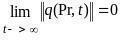
\includegraphics[width=0.8\textwidth]{assets/147}
	\caption*{}
\end{figure}.

Как известно, для определения устойчивости системы (11) анализируются
свойства собственных значений матрицы. Аналогично, для определения
параметрической устойчивости матрицы строится характеристический полином
с коэффициентами, зависящими от параметров \emph{Pr}:

\begin{longtable}[]{@{}
  >{\raggedright\arraybackslash}p{(\columnwidth - 2\tabcolsep) * \real{0.9336}}
  >{\raggedright\arraybackslash}p{(\columnwidth - 2\tabcolsep) * \real{0.0664}}@{}}
\toprule\noalign{}
\begin{minipage}[b]{\linewidth}\raggedright
\(\mathbf{\phi}_{\mathbf{A}}\mathbf{(}\mathbf{\lambda}\mathbf{) =}\mathbf{\det}\mathbf{(}\mathbf{\lambda E}\mathbf{-}\mathbf{A}\mathbf{(}\text{Pr}\mathbf{)) =}\mathbf{p}_{\mathbf{n}}\mathbf{\lambda}^{\mathbf{n}}\mathbf{+}\mathbf{p}_{\mathbf{n}\mathbf{-}\mathbf{1}}\mathbf{\lambda}^{\mathbf{n}\mathbf{-}\mathbf{1}}\mathbf{+ ... +}\mathbf{p}_{\mathbf{0}}\),
\end{minipage} & \begin{minipage}[b]{\linewidth}\raggedright
(12)
\end{minipage} \\
\midrule\noalign{}
\endhead
\bottomrule\noalign{}
\endlastfoot
\end{longtable}

где
\(\mathbf{p}_{\mathbf{i}}\mathbf{,i =}\overline{\mathbf{0,n}}\mathbf{-}\)зависят
от параметров \emph{Pr}.

\emph{Необходимое условие устойчивости:} все коэффициенты
характеристического полинома (12) для фиксированного значения \emph{Pr}
должны находиться в положительной.

Составим матрицу Гурвица

\(\mathbf{M =}\begin{bmatrix}
\mathbf{p}_{\mathbf{1}} & \mathbf{p}_{\mathbf{0}} & \mathbf{0} & \mathbf{0} & \mathbf{...} & \mathbf{0} \\
\mathbf{p}_{\mathbf{3}} & \mathbf{p}_{\mathbf{2}} & \mathbf{p}_{\mathbf{1}} & \mathbf{p}_{\mathbf{0}} & \mathbf{...} & \mathbf{0} \\
\mathbf{...} & \mathbf{...} & \mathbf{...} & \mathbf{...} & \mathbf{...} & \mathbf{...} \\
\mathbf{p}_{\mathbf{2}\mathbf{n}\mathbf{-}\mathbf{1}} & \mathbf{p}_{\mathbf{2}\mathbf{n}\mathbf{-}\mathbf{2}} & \mathbf{p}_{\mathbf{2}\mathbf{n}\mathbf{-}\mathbf{3}} & \mathbf{p}_{\mathbf{2}\mathbf{n}\mathbf{-}\mathbf{4}} & \mathbf{...} & \mathbf{p}_{\mathbf{n}}
\end{bmatrix}\),

где принято \(\mathbf{p}_{\mathbf{j}}\mathbf{= 0}\) при
\(\mathbf{j < 0}\) и \(\mathbf{j > n}\).

Обозначим через
\(\mathbf{\Delta}_{\mathbf{1}}\mathbf{,}\mathbf{\Delta}_{\mathbf{2}}\mathbf{,...,}\mathbf{\Delta}_{\mathbf{n}}\)
главные диагональные миноры матрицы \(\mathbf{M}\):

\[{\mathbf{\Delta}_{\mathbf{1}}\mathbf{=}\mathbf{p}_{\mathbf{1}}\mathbf{,}
}{\mathbf{\Delta}_{\mathbf{2}}\mathbf{=}\left| \begin{matrix}
\mathbf{p}_{\mathbf{1}} & \mathbf{p}_{\mathbf{0}} \\
\mathbf{p}_{\mathbf{3}} & \mathbf{p}_{\mathbf{2}}
\end{matrix} \right|\mathbf{,}
}{\mathbf{.........}
}{\mathbf{\Delta}_{\mathbf{n}}\mathbf{=}\left| \mathbf{M} \right|\mathbf{=}\mathbf{p}_{\mathbf{n}}\mathbf{\Delta}_{\mathbf{n}\mathbf{-}\mathbf{1}}\mathbf{,}}\]

которые в свою очередь являются функциями от параметров \emph{Pr}.

\emph{Критерий параметрической устойчивости Гурвица:} для того чтобы
некоторого значения параметра \emph{Pr} собственные значения матрицы
A(Pr) были
\(\mathbf{Re}\mathbf{\lambda}_{\mathbf{j}}\left( \mathbf{A(}\mathbf{\Pr}\mathbf{)} \right)\mathbf{< 0,j =}\overline{\mathbf{1,n}}\)
необходимо и достаточно, чтобы главные диагональные миноры
\(\mathbf{\Delta}_{\mathbf{1}}\mathbf{,}\mathbf{\Delta}_{\mathbf{2}}\mathbf{,...,}\mathbf{\Delta}_{\mathbf{n}}\)
матрицы \(\mathbf{M}\) находились в правой полуплоскости, т.е.
\(\mathbf{\Delta}_{\mathbf{j}}\mathbf{> 0,j =}\overline{\mathbf{1,n}}\).

Для автоматизированного построения характеристического полинома,
зависящего от параметров \emph{Pr}, на языке MatLab был реализован
алгоритм Леверье-Фадеева, использующий методы компьютерной алгебры. На
основе полученного характеристического полинома формируется матрица
Гурвица, также зависящая от параметров \emph{Pr}. Далее для этой
параметрической матрицы Гурвица вычисляются главные миноры и их
определители.

Используя программу, разработанную на MatLab и представленную ниже,
можно получить следующие результаты линеаризации системы (8).

syms q1 q2 q3 q4 q5 q6 q A B

q0 = \(\lbrack 2.2\ 1.5\ 1.4\ 1.3\ 1.1\ 1.0\rbrack\);

q = {[}q1 q2 q3 q4 q5 q6{]};

t={[}0 10{]}; y0 = q0;

g = 9.8; P = 2000; m = 3; alfa = 30; gamma = 45; Xa = 0.32; Ya = 0.4;

nxa = (P*cos(alfa) - Xa)/(m*g); nya = (P*sin(alfa) + Ya)/(m*g);

F = {[}g*(nxa-sin(q2)); g*(nya*cos(gamma)-cos(q2))/q1;
-g*nya*sin(gamma)/(q1*cos(q2)); q1*cos(q2)*cos(q3); q1*sin(q2);
-q1*cos(q2)*sin(q3){]};

for i=1:length(q0)

for j=1:length(q0)

A(i,j)=diff(F(i),q(j));

end

end

B=subs(A,q,q0);

disp(vpa(A,3));

disp(vpa(B,3));

Представим результат выполнения программы в следующем виде:

\begin{longtable}[]{@{}
  >{\raggedright\arraybackslash}p{(\columnwidth - 2\tabcolsep) * \real{0.9342}}
  >{\raggedright\arraybackslash}p{(\columnwidth - 2\tabcolsep) * \real{0.0658}}@{}}
\toprule\noalign{}
\begin{minipage}[b]{\linewidth}\raggedright
\[A(q) = \frac{\partial f(q,t)}{\partial q} = \begin{pmatrix}
\begin{matrix}
a_{11} & a_{12} \\
a_{21} & a_{22}
\end{matrix} & \begin{matrix}
\ldots & a_{16} \\
\ldots & a_{26}
\end{matrix} \\
\begin{matrix}
\ldots & \ldots \\
a_{61} & a_{62}
\end{matrix} & \begin{matrix}
\ldots & \ldots \\
\ldots & a_{66}
\end{matrix}
\end{pmatrix}\]
\end{minipage} & \begin{minipage}[b]{\linewidth}\raggedright
(13)
\end{minipage} \\
\midrule\noalign{}
\endhead
\bottomrule\noalign{}
\endlastfoot
\end{longtable}

Выпишем только ненулевые элементы матрицы \(A(q)\):

\(a_{12} = - 9.80*cos(q2)\),
\(a_{21} = - 1.*( - 346. - 9.80*cos(q2))/q1\hat{}2\),

\(a_{22} = \ 9.80*sin(q2)/q1\) , \(a_{31} = - 560./q1\hat{}2/cos(q2)\),

\(a_{32} = 60./q1/cos(q2)\hat{}2*sin(q2)\),
\(a_{41} = \ cos(q2)*cos(q3)\),

\(a_{42} = - \ x1*sin(x2)*cos(x3)\), \(a_{43} = - q1*cos(q2)*sin(q3)\),

\(a_{51} = \ sin(q2)\), \(a_{52} = q1*cos(q2)\),
\(a_{61} = - cos(q2)*sin(q3)\),

\(a_{62} = \ q1*sin(q2)*sin(q3)\), \(a_{63} = \  - q1*cos(q2)*cos(q3)\).

Вычислим значение матрицы \(A(q)\) в точке
\(q_{0} = \ \lbrack 2.2\ 1.5\ 1.4\ 1.3\ 1.1\ 1.0\rbrack.\)

\begin{longtable}[]{@{}
  >{\raggedright\arraybackslash}p{(\columnwidth - 2\tabcolsep) * \real{0.9342}}
  >{\raggedright\arraybackslash}p{(\columnwidth - 2\tabcolsep) * \real{0.0658}}@{}}
\toprule\noalign{}
\begin{minipage}[b]{\linewidth}\raggedright
\(A\left( q_{0} \right) = \begin{pmatrix}
\begin{matrix}
0 \\
\begin{matrix}
0.014 \\
\begin{matrix}
0.0. \\
\begin{matrix}
0.012 \\
\begin{matrix}
 - 0.959 \\
 - 0.069
\end{matrix}
\end{matrix}
\end{matrix}
\end{matrix}
\end{matrix} & \begin{matrix}
 - 0.707 \\
\begin{matrix}
0.453 \\
\begin{matrix}
0.0 \\
\begin{matrix}
 - 0.37 \\
\begin{matrix}
0.156 \\
2.162
\end{matrix}
\end{matrix}
\end{matrix}
\end{matrix}
\end{matrix} & \begin{matrix}
\begin{matrix}
0 \\
\begin{matrix}
0 \\
\begin{matrix}
0 \\
\begin{matrix}
0.153 \\
\begin{matrix}
0 \\
0.026
\end{matrix}
\end{matrix}
\end{matrix}
\end{matrix}
\end{matrix} & \begin{matrix}
\begin{matrix}
0 \\
\begin{matrix}
0 \\
\begin{matrix}
0 \\
\begin{matrix}
0 \\
\begin{matrix}
0 \\
0
\end{matrix}
\end{matrix}
\end{matrix}
\end{matrix}
\end{matrix} & \begin{matrix}
\begin{matrix}
0 \\
\begin{matrix}
0 \\
\begin{matrix}
0 \\
\begin{matrix}
0 \\
\begin{matrix}
0 \\
0
\end{matrix}
\end{matrix}
\end{matrix}
\end{matrix}
\end{matrix} & \begin{matrix}
0 \\
\begin{matrix}
0 \\
\begin{matrix}
0 \\
\begin{matrix}
0 \\
\begin{matrix}
0 \\
0
\end{matrix}
\end{matrix}
\end{matrix}
\end{matrix}
\end{matrix}
\end{matrix}
\end{matrix}
\end{matrix}
\end{pmatrix}\).
\end{minipage} & \begin{minipage}[b]{\linewidth}\raggedright
(14)
\end{minipage} \\
\midrule\noalign{}
\endhead
\bottomrule\noalign{}
\endlastfoot
\end{longtable}

В результате работы программы был получен аналитический вид матрицы
\emph{А} и её значение при
\(q_{0} = \ \lbrack 2.2\ 1.5\ 1.4\ 1.3\ 1.1\ 1.0\rbrack\).

В дальнейшем эта матрица \emph{А}, представленная в виде (3.10), была
использована для анализа устойчивости и управляемости модели БПЛА в
заданной точке.

{\bfseries Результаты и обсуждение}. Процесс линеаризации модели (6) для
исходной нелинейной системы (1) оказывается весьма трудоёмким, особенно
при увеличении размерности 𝑛, и становится практически неосуществимым
при n \textgreater{} 3. Более того, при проведении линеаризации часто
проявляется «человеческий фактор», что снижает точность вычислений и не
гарантирует корректности результатов. Это подчеркивает актуальность
задачи автоматизации процесса линеаризации нелинейных моделей {[}8{]}.

Для решения этой проблемы предлагается использовать системы компьютерной
алгебры (СКА), такие как MatLab {[}9-10{]}. Эти системы предоставляют
широкий спектр возможностей для работы с алгебраическими выражениями: от
базовых операций, таких как вычисление и дифференцирование, до более
сложных процедур, включая разложения в ряды и интегрирование. СКА
находят широкое применение в таких областях, как аэрокосмическая
промышленность.

Критерии параметрической устойчивости, изложенные выше, также были
реализованы в приложении, разработанном авторами {[}11{]}.

Результаты численных расчётов полностью согласуются с экспериментальными
данными. Кроме того, результаты сохраняются в текстовые файлы, что
позволяет визуализировать одномерные графики динамики БПЛА с помощью
MatLab, для которого была написана специальная программа.

В качестве перспективного направления можно рассматривать использование
интервальной математики для анализа условий устойчивости БПЛА
{[}12-14{]}.

{\bfseries Выводы.} Статья посвящена исследованию управления и устойчивости
беспилотных летательных аппаратов (БПЛА) с использованием математических
моделей. Основное внимание уделяется линеаризации нелинейных систем
дифференциальных уравнений, описывающих динамику БПЛА, и анализу
устойчивости с применением критерия Гурвица.

Выводы по статье можно сформулировать следующим образом:

\begin{itemize}
\item
  \emph{Значимость беспилотной авиации.} Беспилотные летательные
  аппараты играют важную роль как в военной, так и в гражданской сферах,
  что обусловливает необходимость развития математических моделей для их
  эффективного управления.
\item
  \emph{Нелинейные модели}. Для моделирования динамики БПЛА часто
  используются системы нелинейных дифференциальных уравнений.
  Линеаризация таких моделей является сложной задачей, особенно для
  систем высокой размерности.
\item
  \emph{Автоматизация процесса линеаризации.} Для повышения точности и
  эффективности расчётов предлагается автоматизация процесса
  линеаризации с использованием систем компьютерной алгебры, таких как
  MatLab.
\item
  \emph{Анализ устойчивости.} Устойчивость БПЛА исследуется с
  использованием матрицы Гурвица и критерия параметрической
  устойчивости. Применение метода позволяет выявить условия, при которых
  система будет асимптотически устойчива.
\item
  \emph{Практическая значимость.} Разработанная программа на MatLab
  позволяет автоматизировать процесс построения характеристических
  полиномов и анализа устойчивости, что подтверждено экспериментальными
  результатами.
\item
  \emph{Перспективы.} Одним из направлений дальнейших исследований может
  стать использование интервальной математики для более точного анализа
  устойчивости БПЛА в условиях неопределённости.
\end{itemize}

Таким образом, статья подчеркивает важность применения современных
методов математического моделирования и автоматизации для анализа
устойчивости и управляемости БПЛА.

\emph{{\bfseries Финансирование}. Работа выполнена за счет средств НИИ
математики и механики при КазНУ имени аль-Фараби и грантового
финансирования научных исследований на 2023--2025 годы по проекту
AP19678157.}

{\bfseries Литература}

\begin{enumerate}
\def\labelenumi{\arabic{enumi}.}
\item
  Логинов А.А. Актуальность использования беспилотных летательных
  аппаратов // Актуальные проблемы авиации и космонавтики.- 2015.-Т. 1.-
  С. 704-705
\item
  Хуснутдинов Т.Д., Щербакова А.В., Комарова А.П., Рублевская Е.В.,
  Решетников А.Ю. Перспективы использования беспилотных летательных
  аппаратов в инновационных проектах// Актуальные проблемы авиации и
  космонавтики.- 2017.- Т. 3.- С. 139-141
\end{enumerate}

3.Лю Ш., Ли., Тан Ц., Ву Ш., Годье Ж.-Л. Разработка беспилотных
транспортных средств.- М.:ДМК Пресс.- 2022.-246 с. ISBN
978-5-97060-969-9

4.Августов Л.И и др. Навигация летательных аппаратов в околоземном
пространстве. -- М.: ООО «Научтехлитиздат», 2015. -592с. ISBN
978-5-93728-146-3.

5.Бернс В.А., Долгополов А.В. и др. Экспериментальный модальный анализ
летательных аппаратов. -- Новосибирск: НГТУ, 2023. -- 328 с. ISBN
978-5-7782-3209-9

6.Танг Тхань Лам Системный анализ и оптимизация режимов полета для
управления летательным аппаратом // Автореф. диссер. канд. техн. наук,
спец. 05.13.01, Москва, 2015. -- 155 с.

7. Mazakova A., Jomartova Sh.,Vfzakov T., Shormanov., Amirkhanov B.
Controllability of an unmanned aerial vehicle.// 2022 IEEE 7th
International Energy Conference (ENERGYCON) - C.1-5.
DOI~10.1109/ENERGYCON53164.2022.9830244

8.Mazakova A., Jomartova Sh., Wójcik W., Mazakov T., Ziyatbekova G.
Automated Linearization of a System of Nonlinear Ordinary Differential
Equations// Intl.Journal of electronics and
Telecommunications.-2023.-Vol.69(4).- P.655-660. DOI:
10.24425/ijet.2023.147684

9.Смоленцев Н.К. MatLAb. Программирование на Visual C\#, Borland
JBuilder, VBA. -- М.: ДМК Пресс, 2009. -- 464с.

10.Дьяконов В., Абраменкова И. MATLAB. Обработка сигналов и изображений.
Специальный справочник. -- СПб.: Питер, 2002. - 608 с. ISBN
5-318-00667-1.

11.А.с. №45318 от 2.05.2024 г. Мазақова Ә.Т., Мазаков Т.Ж., Джомартова
Ш.А. Определение устойчивости БПЛА. Программа для ЭВМ.

12.Issimov N., Mazakov T., Mamyrbayev O.,Ziyatbekova G. Application of
fuzzy and interval analysis to the study of the prediction and control
model of the eridemiologic situation// Journal of Theoretical and
Applied information Technology.-Vol.96(14).- P.4358-4368

13. Dzhomartova Sh.A., Mazakov T.Zh, Karymsakova N.T.,Z haydarov A.M.
Comparison of Two Interval Arithmetic// Applied Mathematical
Sciences.-2014.-Vol.8(72).- P.-3593-3598. DOI.10.12988/ams.2014.44301

14.Mazakov T.,Wójcik W.,Jomartova Sh., Karymsakova N.,Ziyatbekova G.,
Tursynbai A. The Stability Interval of the Set of Linear
System//Intl.Journal of electronics and
Telecommunications.-2021.-Vol.67(2).- P.155-161. DOI:
10.24425/ijet.2021.135958

{\bfseries References}

1.Loginov A.A. Aktual\textquotesingle nost\textquotesingle{}
ispol\textquotesingle zovanija bespilotnyh letatel\textquotesingle nyh
apparatov // Aktual\textquotesingle nye problemy aviacii i
kosmonavtiki.- 2015.-T. 1.- S. 704-705.{[}in Russ.{]}

2.Husnutdinov T.D., Shherbakova A.V., Komarova A.P., Rublevskaja E.V.,
Reshetnikov A.Ju. Perspektivy ispol\textquotesingle zovanija bespilotnyh
letatel\textquotesingle nyh apparatov v innovacionnyh proektah//
Aktual\textquotesingle nye problemy aviacii i kosmonavtiki.- 2017.- T.
3.- S. 139-141.{[}in Russ.{]}

3.Lju Sh., Li., Tan C., Vu Sh., God\textquotesingle e Zh.-L. Razrabotka
bespilotnyh transportnyh sredstv.- M.:DMK Press.- 2022.-246 s. ISBN
978-5-97060-969-9.{[}in Russ.{]}

4.Avgustov L.I i dr. Navigacija letatel\textquotesingle nyh apparatov v
okolozemnom prostranstve. -- M.: OOO «Nauchtehlitizdat», 2015. -592s.
ISBN 978-5-93728-146-3. {[}in Russ.{]}

5.Berns V.A., Dolgopolov A.V. i dr. Jeksperimental\textquotesingle nyj
modal\textquotesingle nyj analiz letatel\textquotesingle nyh apparatov.
-- Novosibirsk: NGTU, 2023. -- 328 s. ISBN 978-5-7782-3209-9.{[}in
Russ.{]}

6.Tang Than\textquotesingle{} Lam Sistemnyj analiz i optimizacija
rezhimov poleta dlja upravlenija letatel\textquotesingle nym apparatom
// Avtoref. disser. kand. tehn. nauk, spec. 05.13.01, Moskva, 2015.-155
s. {[}in Russ.{]}

7. Mazakova A., Jomartova Sh.,Vfzakov T., Shormanov., Amirkhanov B.
Controllability of an unmanned aerial vehicle.// 2022 IEEE 7th
International Energy Conference (ENERGYCON) - C.1-5.
DOI~10.1109/ENERGYCON53164.2022.9830244

8.Mazakova A., Jomartova Sh., Wójcik W., Mazakov T., Ziyatbekova G.
Automated Linearization of a System of Nonlinear Ordinary Differential
Equations// Intl.Journal of electronics and
Telecommunications.-2023.-Vol.69(4).- P.655-660. DOI:
10.24425/ijet.2023.147684

9.Smolencev N.K. MatLAb. Programmirovanie na Visual C\#, Borland
JBuilder, VBA. -- M.: DMK Press, 2009. -- 464 s. {[}in Russ.{]}

10.D\textquotesingle jakonov V., Abramenkova I. MATLAB. Obrabotka
signalov i izobrazhenij. Special\textquotesingle nyj spravochnik. --
SPb.: Piter, 2002. - 608 s. ISBN 5-318-00667-1. {[}in Russ.{]}

11.A.s. №45318 ot 2.05.2024 g. Mazaқova Ә.T., Mazakov T.Zh., Dzhomartova
Sh.A. Opredelenie ustojchivosti BPLA. Programma dlja JeVM. {[}in
Russ.{]}

12.Issimov N., Mazakov T., Mamyrbayev O.,Ziyatbekova G. Application of
fuzzy and interval analysis to the study of the prediction and control
model of the eridemiologic situation// Journal of Theoretical and
Applied information Technology.-Vol.96(14).- P.4358-4368

13. Dzhomartova Sh.A., Mazakov T.Zh, Karymsakova N.T.,Z haydarov A.M.
Comparison of Two Interval Arithmetic// Applied Mathematical
Sciences.-2014.-Vol.8(72).- P.-3593-3598. DOI.10.12988/ams.2014.44301

14.Mazakov T.,Wójcik W.,Jomartova Sh., Karymsakova N.,Ziyatbekova G.,
Tursynbai A. The Stability Interval of the Set of Linear
System//Intl.Journal of electronics and
Telecommunications.-2021.-Vol.67(2).- P.155-161. DOI:
10.24425/ijet.2021.135958

\emph{{\bfseries Сведение об авторах}}

Мазақова А.Т. -- докторант Казахского национального университета
им.аль-Фараби, Алматы, Казахстан, e-mail: aigerym97@mail.ru;

Джомартова Ш.А. - доктор технических наук, доцент, Казахский
национальный университет им. аль-Фараби, Алматы, Казахстан, e-mail:
jomartova@mail.ru;

Мазаков Т.Ж. -- доктор физико-математических наук, профессор, Казахский
национальный университетим. аль-Фараби, Алматы, Казахстан, e-mail:
tmazakov@mail.ru;

Тойкенов Г.Ч. - кандидат физико-математических наук, доцент, Казахский
национальный женский педагогический университет, Алматы, Казахстан,
e-mail: gumyrbektoike@mail.ru;

Әлиасқар М.С. - докторант Казахского национального университета
им.аль-Фараби, Алматы, Казахстан, e-mail: m.alyasqar@gmail.ru

\emph{{\bfseries Information about the authors}}

Mazakova A.T. - PhD student of the Al-Farabi Kazakh National University,
Almaty, Kazakhstan, e-mail: aigerym97@mail.ru;

Jomartova Sh.A. - Doctor of Technical Sciences, Associate Professor,
Al-Farabi Kazakh National University, Almaty, Kazakhstan, e-mail:
jomartova@mail.ru;

Mazakov T.Zh. -- Doctor of Physical and mathematical sciences,
professor, Al-Farabi Kazakh National University, Almaty, Kazakhstan,
e-mail: tmazakov@mail.ru;

Tokenov G.Ch. - Candidate of Physical and Mathematical Sciences,
Associate Professor, Kazakh National Women\textquotesingle s Pedagogical
University, Almaty, Kazakhstan, e-mail: gumyrbektoike@mail.ru;

Aliaskar M.S. - Lecturer at the International University of Engineering
and Technology, Almaty, Kazakhstan, e-mail: m.alyasqar@gmail.ru\newpage
{\bfseries МРНТИ 44.01.81}

{\bfseries Разработка микропроцессорной системы передачи данных для
мониторинга нагрузки электроэнергетических систем}

{\bfseries \textsuperscript{1}Г.И. Жолдангарова, \textsuperscript{2,3}М.Н.
Калимолдаев, \textsuperscript{4,5}В.Б. Барахнин,
\textsuperscript{2,3}Г.З. Зиятбекова\textsuperscript{🖂},}

{\bfseries \textsuperscript{3}М.Т. Аршидинова}

\textsuperscript{1}Евразийский национальный университет имени Л.Н.
Гумилева, Астана, Казахстан,

\textsuperscript{2}Казахский национальный университет имени аль-Фараби,
Алматы, Казахстан,

\textsuperscript{3}Институт информационных и вычислительных технологий,
КН МНВО РК,

Алматы, Казахстан,

\textsuperscript{4}Федеральный исследовательский центр информационных и
вычислительных технологий, Новосибирск, Россия,

\textsuperscript{5}Новосибирский государственный университет,
Новосибирск, Россия

{\bfseries \textsuperscript{🖂}}Корреспондент-автор: ziyatbekova@mail.ru

В статье рассматривается разработка микропроцессорной системы для
мониторинга нагрузки электроэнергетических систем на основе технологий
IoT. Приведен обзор научных исследований в данной области. В качестве
пилотного прототипа разработана микропроцессорная система измерения
климатических параметров, а также напряжения и тока. Система
предназначена для обеспечения эффективного контроля и управления
тепловым насосом и связанным оборудованием. Построена информационная
схема, которая описывает взаимодействие между компонентами системы
мониторинга нагрузки электроэнергетических систем и потоки информации от
датчиков до конечного хранения данных.

{\bfseries Ключевые слова:} микропроцессорная система, датчик,
микрокомпьютер Raspberry, контроллер, платформа Arduino MEGA и FPGA.

{\bfseries ЭЛЕКТР ЭНЕРГЕТИКАЛЫҚ ЖҮЙЕЛЕРДІҢ ЖҮКТЕМЕСІН БАҚЫЛАУ ҮШІН
ДЕРЕКТЕРДІ БЕРУДІҢ МИКРОПРОЦЕССОРЛЫҚ ЖҮЙЕСІН ӘЗІРЛЕУ}

{\bfseries \textsuperscript{1}Г.И. Жолдангарова, \textsuperscript{2,3}М.Н.
Калимолдаев, \textsuperscript{4,5}В.Б. Барахнин,
\textsuperscript{2,3}Г.З. Зиятбекова\textsuperscript{🖂},}

{\bfseries \textsuperscript{3}М.Т. Аршидинова}

\textsuperscript{1}Л.Н. Гумилев атындағы Еуразия ұлттық университеті,
Астана, Қазақстан,

\textsuperscript{2}әл-Фараби атындағы Қазақ ұлттық университеті, Алматы,
Қазақстан,

\textsuperscript{3}Ақпараттық және есептеуіш технологиялар институты, ҚР
ҒК ҒЖБМ, Алматы, Қазақстан,

\textsuperscript{4}Ақпараттық және есептеу технологияларын Федералды
зерттеу орталығы,

Новосибирск, Ресей,

\textsuperscript{5}Новосибирск мемлекеттік университеті, Новосибирск,
Ресей,

е-mail: igibaevna@bk.ru

Мақалада IoT технологияларына негізделген электр энергетикалық
жүйелерінің жүктемесін бақылауға арналған микропроцессорлық жүйенің
дамуы қарастырылады. Осы саладағы ғылыми зерттеулерге шолу жасалған.
Пилоттық прототип ретінде климаттық параметрлерді, сондай-ақ кернеу мен
токты өлшейтін микропроцессорлық жүйе жасалды. Жүйе жылу сорғысымен
байланысты жабдықты тиімді бақылау мен басқаруды қамтамасыз етуге
арналған. Электр энергетикалық жүйелердің жүктемесін бақылау жүйесінің
компоненттері мен cенсорлардан деректерді соңғы сақтауға дейінгі ақпарат
ағындары арасындағы өзара әрекеттесуді сипаттайтын ақпараттық схема
құрылды.

{\bfseries Түйін сөздер:} микропроцессорлық жүйе, сенсор, Raspberry
микрокомпьютері, контроллер, Arduino Mega платформасы және FPGA.

{\bfseries DEVELOPMENT OF A MICROPROCESSOR-BASED DATA TRANSMISSION SYSTEM
FOR LOAD MONITORING OF ELECTRIC POWER SYSTEMS}

{\bfseries \textsuperscript{1}G.I. Zholdangarova, \textsuperscript{2,3}M.N.
Kalimoldayev, \textsuperscript{4,5}V.B. Barakhnin,
\textsuperscript{2,3}G.Z. Ziyatbekova\textsuperscript{🖂},}

{\bfseries \textsuperscript{3}М.Т. Arshidinova}

\textsuperscript{1}L.N. Gumilyov Eurasian National University, Astana,
Kazakhstan,

\textsuperscript{2}Al-Farabi Kazakh National University, Almaty,
Kazakhstan,

\textsuperscript{3}Institute of Information and Computational
Technologies CS MSHE RK, Almaty, Kazakhstan,

\textsuperscript{4}Federal Research Center for Information and
Computational Technologies, Novosibirsk, Russia,

\textsuperscript{5}Novosibirsk State University, Novosibirsk, Russia,

е-mail: igibaevna@bk.ru

The paper deals with the development of a microprocessor-based system
for load monitoring of electric power systems based on IoT technologies.
An overview of scientific research in the field is given. A
microprocessor-based system for measuring climatic parameters as well as
voltage and current has been developed as a pilot prototype. The system
is designed to provide effective monitoring and control of the heat pump
and related equipment. An information scheme is constructed that
describes the interaction between components of the power system load
monitoring system and the information flows from the sensors to the
final data storage system.

{\bfseries Key words:} microprocessor system, sensor, Raspberry
microcomputer, controller, Arduino MEGA and FPGA platform.

{\bfseries Введение.} Рост населения и экономики Республики Казахстан
приводит к огромному спросу на электроэнергию и энергетические ресурсы.
Как отмечают аналитики казахстанской версии журнала «Forbes», в целом по
стране наблюдается дефицит электроэнергии, что делает энергетический
сектор уязвимым. Казахстан столкнулся с дефицитом электрической энергии
и мощности, который в вечерние часы составляет более 1,3 ГВт. В
региональном же разрезе, особенно в южной зоне, дефицит электроэнергии
серьёзно подрывает энергетическую безопасность страны. Только в марте
2023 года в Южном Казахстане производство компенсировало всего 57,2\%
потребления --- дефицит составил 971,0 млн кВт·ч.

В сложившихся условиях важно иметь инструмент для мониторинга нагрузки в
энергосистеме с целью выявления на его основе возможного развития
критических ситуаций, чтобы иметь возможность принимать управленческие
решения для недопущения их возникновения. Эффективным методом решения
данной задачи является использования технологий Интернета вещей (IoT)
для мониторинга процессов в энергосистеме {[}1{]}, сочетающего в себе
несколько методов анализа и прогнозирования данных о потреблении
электроэнергии {[}2{]}.

Использование IoT в энергетическом секторе относится к числу бурно
развивающихся в настоящее время технологий. Нашим вкладом в развитие
этой области будет разработка встроенного контроллера Arduino MEGA и
FPGA. Все критические параметры на подстанции, включая напряжение,
частоту, мощность, состояние выключателя и температуру внутри системы,
контролируются с его использованием посредством занесения в базу данных
веб-сервера для последующего анализа. Предопределенные механизмы запуска
событий также запрограммированы на контроллере с функциями записи:
данные записываются контроллером и передаются на веб-сервер с помощью
микроконтроллера ESP32. Контроллер, встроенный в FPGA, обеспечивает
высокоскоростные и надежные функции сбора и обработки данных.

Информационные системы имеют преимущества по сравнению с традиционными
методами мониторинга. Они способны выявлять сложные закономерности в
данных, что повышает точность прогнозов. В целом разработка этой
информационной системы открывает перспективы для повышения надежности и
эффективности энергосистем.

Стратегической целью этой программы является разработка информационной
системы для мониторинга нагрузки электроэнергетических сетей на основе
IoT-технологий, использующих встроенный контроллер Arduino MEGA и FPGA
для мониторинга на подстанции напряжения, частоты, мощности, состояния
выключателя, температуры внутри системы.

Микропроцессорная система включает в себя следующие компоненты:

\begin{itemize}
\item
  Модуль сбора данных: Сбор данных о нагрузке и других параметрах сети с
  помощью датчиков IoT.
\item
  Модуль очистки данных: Предварительная обработка данных для удаления
  шумов и выбросов.
\item
  Модуль представления результатов: Формирование отчетов и визуализация
  результатов прогнозирования.
\end{itemize}

{\bfseries Литературный обзор.} Интернет вещей (IoT) стал революционной
технологией в области мониторинга энергосетей {[}3, 4{]}. Благодаря
решению проблем и использованию возможностей FPGA продолжит
трансформировать энергетический сектор {[}5{]}. B {[}6, 7, 8{]} статьи
охватывают широкий спектр тем, включая приложения IoT для мониторинга
нагрузки, преимущества и проблемы использования IoT, а также будущие
направления развития в Республике Казахстан.

Прежде всего, отметим статью {[}8{]} академика М.Н. Калимолдаева,
которая вносит весомый вклад в разработку информационных систем с
интегрированными модулями машинного обучения для робототехники и
автоматизации. Идеи этой статьи получают дальнейшее развитие в данной
работе. Направление исследований определяется тем, что Интернет вещей в
последнее время приобрел широкое распространение. Так в статье {[}9{]}
представлен подход на основе Интернета вещей к решению проблем
энергетики.

Данное исследование реализовано для удовлетворения этих потребностей
путем разработки нового интеллектуального датчика FPGA. Указанный подход
для решения различных задач описан в работах {[}10, 11, 12, 13, 14{]}.

Многократное выполнение прикладной программы отнимает огромное
количество времени. Чтобы сократить время выполнения, в статье {[}15{]}
предлагается использовать адаптивную модель.

Автор в {[}16{]} предположил, что использование технологии Fog/Edge
может обеспечить решение таких проблем, как осуществимость Интернета
вещей (соображения безопасности в отношении вычислений и стоимости
системы) и будущая осуществимость (надлежащее проектирование
инфраструктуры для будущих приложений).

Управление электроприборами включает в себя сбор и анализ данных об их
энергопотреблении, оптимизацию графиков их работы, расчет показателей
энергопотребления и реализацию решений по оптимизации энергопотребления
{[}17{]}.

Статьи {[}18, 19, 20, 21{]} содержат ценную информацию об использовании
Интернета вещей для повышения эффективности и надежности
электроэнергетических сетей посредством мониторинга нагрузки.

Вот некоторые ключевые выводы из этих статей:

- Технологии Интернета вещей могут значительно повысить точность
мониторинга и прогнозирования нагрузки.

- Системы на базе Интернета вещей могут собирать данные в режиме
реального времени из широкого спектра источников, которые можно
использовать для разработки более точных моделей нагрузки.

- Системы на базе Интернета вещей можно использовать для выявления
событий экстремальной нагрузки, что может помочь предотвратить перебои в
подаче электроэнергии.

- Системы на базе Интернета вещей можно использовать для оптимизации
энергопотребления, что может помочь снизить затраты и воздействие на
окружающую среду.

{\bfseries Материалы и методы.} Рассмотрена методика экспериментальных
исследований, описан процесс обработки результатов измерения.

{\bfseries Результаты и дискуссия.}

\emph{Этап 1. Для начального этапа, разработки умной системы для
мониторинга электропотребления,} уровни Технологической Готовности (TRL)
могут быть описаны следующим образом:

\begin{itemize}
\item
  теоретическое исследование возможностей интеграции датчиков IoT и
  интеллектуальных счетчиков;
\item
  разработка и тестирование первичных версий системы с использованием
  реальных данных в лабораторных условиях;
\item
  анализ данных и предоставление информации о потреблении электроэнергии
  пользователям.
\end{itemize}

Каждый этап TRL требует определенных исследований, разработок и
тестирований, а также постепенного увеличения масштаба и их сложности.
Это обеспечивает систематический подход к разработке и внедрению
технологии.

\emph{Этап 2. Разработка высокоскоростной системы сбора и обработки
данных контроллера.}

На втором этапе контроллер, встроенный в FPGA, обеспечивает
высокоскоростной и надежный сбор и обработку данных. Сбор данных
осуществляется с помощью датчиков Zmpt101b и ACQ720. Благодаря высокой
частоте дискретизации системы как установившиеся, так и переходные
режимы энергосистемы контролируются с использованием одного источника
времени. С помощью платформы IoT данные передаются через локальную сеть
для записи в базу данных. Критерием успешной реализации будет точность,
надежность и производительность системы.

Технологическая готовность определяется наличием высокоскоростной
системы сбора и обработки данных контроллера в составе
полнофункционального макета информационной системы мониторинга нагрузки
электроэнергетических сетей -- индекс готовности {[}22, 23{]}.

\emph{Этап 3. Разработка методов и протоколов связи, а также необходимых
мер кибербезопасности для занесения на сервер данных встроенного
контроллера Arduino MEGA и FPGA.}

Основными принципами исследования являются существующие технологии и
методы передачи данных и кибербезопасности. Теоретическая разработка
концепции протоколов связи и мер кибербезопасности для Arduino MEGA и
FPGA.

TRL включает в себя углубление исследований, разработок и тестирований,
обеспечивая поэтапный и систематический подход к разработке и внедрению
технологии в реальные условия.

\begin{figure}[H]
	\centering
	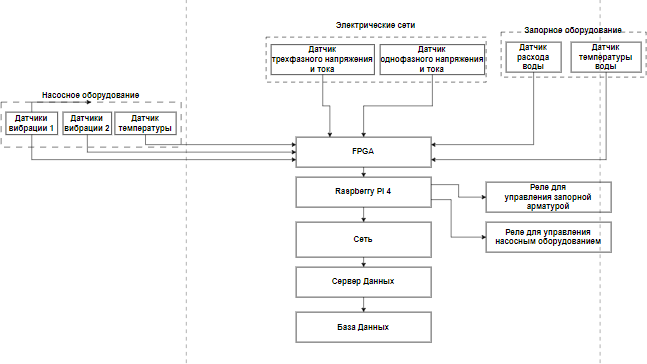
\includegraphics[width=0.8\textwidth]{assets/148}
	\caption*{}
\end{figure}

{\bfseries Рис. 1 - Структурная схема системы}

Опишем пилотный прототип создаваемой системы, предназначенный для
обеспечения эффективного контроля и управления тепловым насосом и
связанным оборудованием, основная задача которого -- сбор данных от
датчиков, их обработка и использование для управления насосом и запорной
арматурой в реальном времени. Информационная схема описывает
взаимодействие между компонентами системы и потоком информации от
датчиков до конечного хранения данных (Рисунок 1).

\emph{Описание компонентов и их взаимодействия}

\emph{Датчики:}

\begin{itemize}
\item
  Датчики вибрации 1 и 2 устанавливаются на корпусе насоса и ближе к
  ротору, чтобы измерять вибрации, которые могут указывать на возможные
  механические неисправности или износ.
\item
  Датчик температуры монтируется на корпусе насоса рядом с подшипниками,
  отслеживая его рабочую температуру для предотвращения перегрева.
\item
  Датчик трёхфазного напряжения и тока измеряет параметры трехфазных
  цепей, что позволяет контролировать (для мониторинга) нагрузку и
  напряжение.
\item
  Датчик однофазного напряжения и тока контролирует однофазные цепи,
  обеспечивая дополнительную информацию о состоянии системы.
\item
  Датчик расхода воды измеряет объем или поток воды, проходящей через
  насос, чтобы обеспечить его оптимальную работу и предотвратить
  возможные проблемы.
\item
  Датчик температуры воды контролирует температуру воды в системе, что
  важно для управления процессами и предотвращения перегрева.
\end{itemize}

\emph{Сбор данных:} Все датчики передают данные на Raspberry Pi 4 через
FPGA, который выполняет первичную обработку всех данных (вибрации,
температуры, напряжения и тока), т.е. регулярно отправляют свои
показания.

\emph{Устройства управления:}

\begin{itemize}
\item
  Реле для управления запорной арматурой управляет клапанами и запорной
  арматурой в системе, контролируя потоки жидкости и обеспечивая их
  правильное направление.
\item
  Реле для управления насосом включает/выключает насос в зависимости от
  условий работы, заданных в программном обеспечении Raspberry Pi 4. Это
  позволяет автоматически регулировать работу насоса в ответ на
  изменения в системе. Raspberry Pi 4 отправляет команды на реле для
  управления насосом и запорной арматурой, основываясь на полученных
  данных и выполненном анализе.
\end{itemize}

Команды управления реле (для запорной арматуры и насоса) формируются на
основе данных от датчиков и логики управления.

\emph{FPGA:}

\begin{itemize}
\item
  FPGA получает данные от всех датчиков (вибрация, температура,
  трехфазное и однофазное напряжение и ток).
\item
  Выполняет первичную обработку данных, включая фильтрацию и
  сглаживание.
\item
  Обработанные данные передаются на Raspberry Pi 4.
\end{itemize}

\emph{Контроллер:}

\begin{itemize}
\item
  Raspberry Pi 4 (центральный контроллер системы)
\end{itemize}

Платформа IoT основана на базе Raspberry Pi 4, которая является основной
в системе и необходима для обработки данных; управления реле и передачи
данных через сеть. Данные могут быть переданы на сервер для хранения и
анализа. Сервер базы данных принимает данные от платформы IoT и
сохраняет их для дальнейшего отображения в ситуационном центре, анализа
и отчетности.

Raspberry Pi 4 и FPGA выступает в роли центрального контроллера системы.
Они принимают данные от всех датчиков через соответствующие интерфейсы
(GPIO, SPI, I2C или USB). Raspberry Pi 4 обрабатывает данные, выполняет
вычисления и принимает решения на основе предустановленных алгоритмов.

\emph{Обработка данных:} Raspberry Pi 4 через FPGA получает данные от
датчиков, обрабатывает их в реальном времени, используя установленные
алгоритмы и логические правила. На основе анализа данных принимаются
решения о необходимости включения или выключения насосов и управления
запорной арматурой.

\emph{Интерфейсы и связи:}

\begin{itemize}
\item
  Интерфейсы датчиков (например, аналоговые выходы, цифровые сигналы)
\item
  SPI/I2C/USB (интерфейсы для подключения датчиков и реле к Raspberry Pi
  4)
\item
  Ethernet/Wi-Fi (для передачи данных в локальную сеть)
\end{itemize}

\emph{Платформа IoT:}

\begin{itemize}
\item
  Локальная сеть (LAN)
\item
  Сервер данных (для хранения и обработки данных)
\end{itemize}

Данные от Raspberry Pi 4 передаются в локальную сеть (LAN) через
Ethernet или Wi-Fi. Платформа IoT в сети обеспечивает связь между
Raspberry Pi 4 и сервером данных. Сервер данных принимает и хранит
данные, переданные от Raspberry Pi 4. Это может включать в себя хранение
исторических данных, обработку информации и выполнение аналитики.

\emph{База данных:}

Сервер базы данных (например, SQL или NoSQL база данных для хранения
данных). База данных на сервере служит для долговременного хранения
данных. Здесь сохраняются все данные, полученные от датчиков и
обработанные контроллером. База данных также используется для
формирования отчетов и анализа состояния системы. Обработанные данные
передаются в локальную сеть, затем на сервер данных, где сохраняются в
базе данных. Данные могут быть использованы для последующего анализа,
формирования отчетов и оптимизации работы системы.

\emph{Реляционная база данных (SQL). Форматы и таблицы:}

\emph{Таблица sensor\_data:}

\begin{itemize}
\item
  id (INT, PK) --- Уникальный идентификатор записи
\item
  timestamp (TIMESTAMP) --- Время измерения
\item
  sensor\_type (VARCHAR) --- Тип датчика (вибрация, температура,
  напряжение и т.д.)
\item
  sensor\_location (VARCHAR) --- Местоположение датчика (например,
  корпус насоса, ротор и т.д.)
\item
  value (FLOAT) --- Значение измерения
\end{itemize}

\emph{Таблица device\_control:}

\begin{itemize}
\item
  id (INT, PK) --- Уникальный идентификатор записи
\item
  timestamp (TIMESTAMP) --- Время управления
\item
  device\_type (VARCHAR) --- Тип устройства (например, насос, запорная
  арматура)
\item
  action (VARCHAR) --- Действие (включить/выключить)
\end{itemize}

\emph{Таблица system\_logs:}

\begin{itemize}
\item
  id (INT, PK) --- Уникальный идентификатор записи
\item
  timestamp (TIMESTAMP) --- Время события
\item
  log\_type (VARCHAR) --- Тип лога (ошибка, предупреждение и т.д.)
\item
  message (TEXT) --- Сообщение лога
\end{itemize}

\emph{Преимущества:}

\begin{itemize}
\item
  Хорошо структурированы данные.
\item
  Поддержка сложных запросов и транзакций.
\item
  Хорошая поддержка для аналитики и отчетности.
\end{itemize}

Приступим к описанию разрабатываемой система мониторинга
электропотребления. Предлагается следующая ее схема, состоящая из трех
блоков:

1) блок приема и передачи текущей информации (вибрации, температуры,
напряжения и тока);

2) блок обработки постоянной и оперативной информации об угрозе аварии
(сервер);

3) блок прогнозирования аварийных ситуаций в энергосистемах.

Основной информацией для мониторинга нагрузки электроэнергетических
систем являются данные, поступающие от датчиков, показанных на рисунке
1. Дополнительную информацию дают данные с датчиков через
соответствующие интерфейсы. Блок приема-передачи текущей информации
реализован в виде датчиков вибрации, температуры, напряжения и тока.
Датчики подключены к микропроцессору Arduino, который обеспечивает
предварительную обработку поступающих с датчиков данных и передает их
для дальнейшей обработки. Используется устройство на базе
микроконтроллера ATmega 328. В комплект поставки входит все необходимое
для удобной работы с микроконтроллером. Для начала работы с устройством
достаточно подать питание от адаптера переменного/постоянного тока или
аккумулятора, либо подключить его к компьютеру с помощью USB-кабеля.

Блок обработки постоянной и оперативной информации об угрозе аварийных
ситуаций содержит постоянную информацию о характеристиках энергосистемы,
а также оперативно получает текущую информацию, на основе обработки
которой блок рассчитывает уровень безопасности, тревожности или
катастрофичности электроэнергетического комплекса. В последнем случае он
автоматически оповещает государственные органы (МЧС, акиматы и т.д.) о
возможной угрозе аварии.

{\bfseries Выводы.} В целом использование Интернета вещей для мониторинга
нагрузки электроэнергетических сетей является быстро развивающейся
областью исследований, которая потенциально может оказать существенное
влияние на энергетический сектор.

Дано описание разработанной в Казахстане технологии мониторинга нагрузки
электроэнергетических систем, обсуждены результаты ее практического
использования в отдельных регионах и намечены направления дальнейшего
развития. Сформулированы цель и основные задачи исследований,
направленных на разработку методики прогнозирования
электроэнергетической аварии как чрезвычайной ситуации на основе анализа
различных существующих методов. Использован метод непрерывной волны или
метод ультразвукового импульсного эха. В качестве пилотного прототипа
разработана автономная микрокомпьютерная система передачи климатических
данных на основе микропроцессорной техники и датчиков. Разработана
программа мониторинга факторов волн нагрузки в режиме реального времени
для датчиков определения уровня безопасности.

\emph{{\bfseries Финансирование.}} Работа выполнена за счет средств
грантового финансирования научных исследований на 2024-2026 годы по
проекту АР23490529 «Разработка информационной системы и математических
моделей для мониторинга и прогнозирования нагрузки электроэнергетических
систем на основе гибридных технологий».

{\bfseries Литература}

1.Ahmed N., De D., Hussain M. I. Internet of things (IoT) for smart
precision agriculture and farming in rural areas // IEEE Internet of
Things Journal. 2018. Vol. 5(6)- P. 4890- 4899.

DOI 10.1109/JIOT.2018.2879579

2. Liangzhi Li, Kaoru Ota, Mianxiong Dong. When Weather Matters:
IoT-Based Electrical Load Forecasting for Smart Grid // IEEE
Communications Magazine, 2017. -- Vol. 5(10).- P. 46-51. DOI
10.1109/MCOM.2017.1700168

3.Prasanna Hambarde, Rachit Varma, Shivani Jha. The Survey of Real Time
Operating System: RTOS. -- IEEE International Conference on Electronic
Systems, Signal Processing and Computing Technologies, 2014. DOI
10.1109/ICESC.2014.15

4. Kalimoldayev M., Akhmetzhanov М., Kunelbayev М., Sundetov Т.
Information systems of integrated machine learning modules on the
example of a verbal robot // News of the National Academy of sciences of
the Republic of Kazakhstan. Series of geology and technical sciences,
2019. -No. 6(438).- P. 215-222. DOI 10.32014/2019.2518-170X.173

5.Kalimoldayev M., Tynymbayev S., Magzom M., Tananova D., Lyshevski S.
FPGA Implementation of Encryption Algorithms Based on Residual
Polynomials // 2020 IEEE 40th International Conference on Electronics
and Nanotechnology (ELNANO), IEEE, Kyiv, Ukraine, 2020. DOI
10.1109/ELNANO50318.2020.9088890

6.Kalimoldayev M., Akhmetzhanov M., Kunelbayev M. Determination of the
power interaction of the hydro turbine GRID with a fluid flow for a
double-rotor micro hydro power plant // Известия НАН РК. Серия
физико-математическая, 2019. -- No. 4. -- P. 59-67.

DOI 10.32014/2019.2518-1726.4

7.Kalimoldayev M., Akhmetzhanov M., Kunelbayev M. Development and
research of a mathematical model of a solar photo converter with an
inverter for converting direct current to alternating voltage //
Известия НАН РК. Серия физико-математическая, 2019. -- No. 4. -- P.
135-142. DOI 10.32014/2019.2518-1726.52

8.Kalimoldayev M.N., Pak I. T.,Baipakbayeva S., Mun G., Shaltykova D.
B., I. E. Suleimenov

Methodological basis for the development strategy of artificial
intelligence systems in the Republic of Kazakhstan in the message of the
president of the Republic of Kazakhstan // News of the National Academy
of Sciences of the Republic of the Kazakhstan. Series of geology and
technical sciences, 2018. -- Vol. 6. -- P. 47-54. DOI
10.32014/2018.2518-170X.34

9.Kalimoldayev M.N., Abdildayeva A., Zhukabayeva T., Turaev Sh. The
investigation of the

internet of things (IoT) in electric power systems // News of the
National Academy of Sciences of the Republic of Kazakhstan. Series of
Geology and Technical Sciences, 2019. -- Vol. 5. -- No. 437. -- P.
144-150. DOI 10.32014/2019.2518-170X.136

10.{[}online{]} Available: http://www.ni.com/fpga/ (17.07.2024)

11.Introduction to FPGA technology: Top 5 benefits, {[}online{]}
Available: http://www.ni.com/white-paper/6984/en/ (13.05.2024)

12.Hao Z., Lianping G., Jie M., and Peng Y. Research on the hardware
co-processing technology for waveform character searching with a digital
oscilloscope, Proc. 13th IEEE Int. Conf. Electron. Meas. Instrum,
2017.-P. 92-97. DOI 10.1109/ICEMI.2017.8265920

13.Escobar F.A., Chang X., and Valderrama C. Suitability analysis of
FPGAs for heterogeneous platforms in HPC, IEEE Trans. -- Parallel
Distrib. Syst. 2016, -- Vol. 27(2). -- P. 600-612.

DOI 10.1109/TPDS.2015.2407896

14.Sheng J., Yang C., Sanaullah A., Papamichael M., Caulfield A., and
Herbordt M.C. HPC on FPGA clouds: 3D FFTs and implications for molecular
dynamics, 2017. -- Proc. 27th Int. Conf. Field Program. Logic Appl. DOI
10.23919/FPL.2017.8056853

15.Chen R., and Prasanna V.K. Computer generation of high throughput and
memory efficient sorting designs on FPGA, IEEE Trans. -- Parallel
Distrib. Syst. 2017. -- Vol. 28. -- No. 11. -- P. 3100-3113.
DOI:~10.1109/TPDS.2017.2705128

16.Хироаки Н. Information and communication platform for providing smart
community services: System implementation and use case in Saitama city
// Proceedings of the IEEE International Conference on Industrial
Technology, 2018. -- Р. 1375-1380. DOI 10.1109/ICIT.2018.8352380.

17.Hussien N. Ali, Daleh Al-Magsoosi A.A., AlRikabi S., Abed F.T.
Monitoring the Consumption of Electrical Energy Based on the Internet of
Things Applications // International Journal of Interactive Mobile
Technologies.- 2021.-Vol.15(07). DOI 10.3991/ijim.v15i07.20183.

18.Motlagh N.H., Mohammadrezaei M., Hunt J., Zakeri B. Internet of
Things (IoT) and the Energy Sector // Energies, 2020.
DOI:10.3390/en13020494

19.Liu Hua, Junguo Zhang, Lin Fantao. Internet of Things Technology and
its Applications in Smart Grid // TELKOMNIKA Indonesian Journal of
Electrical Engineering.- 2014.-Vol. 12. (2)- DOI
10.11591/telkomnika.v12i2.4178

20.Tanveer Ahmad, Dongdong Zhang. Using the internet of things in smart
energy systems and networks //Sustainable Cities and Society.-
2021.-Vol. 68. DOI 10.1016/j.scs.2021.102783

21.Mohammad Kamrul Hasan, Musse Mohamud Ahmed, Bishwajeet Pandey, Hardik
Gohel, Shayla Islam, Izzul Fitrie Khalid. Internet of Things-Based Smart
Electricity Monitoring and Control System Using Usage Data // Wireless
Communications and Mobile Computing.- 2021.

- P.1-16/ DOI 10.1155/2021/6544649

21.Suryanarayanan A., Ramamurthy A., Chaudhry A.K. Internet of Things
for monitoring and forecasting the load Electric Power Networks: Future
Directions. IEEE Access Journal, 2021. -- Vol. 9. -- Pp. 136350-136379

22.Chen C., Li K., Duan M. Chapter 6. Extreme Learning Machine and Its
Applications in Big Data Processing. Big Data Analytics for
Sensor-Network Collected Intelligence Intelligent Data-Centric Systems,
2017. -- Pp. 117-150. https://doi.org/10.1016/B978-0-12-809393-1.00006-4

23.Heddam S., Kim S., Mehr A., Zounemat-Kermani M. Chapter 11. A long
short-term memory deep learning approach for river water temperature
prediction. Current Trends and Advances in Computer-Aided Intelligent
Environmental Data Engineering Intelligent Data-Centric Systems, 2022. -
P. 243-270. https://doi.org/10.1016/B978-0-323-85597-6.00015-X.

{\bfseries References}

1.Ahmed N., De D., Hussain M. I. Internet of things (IoT) for smart
precision agriculture and farming in rural areas // IEEE Internet of
Things Journal. 2018. Vol. 5(6)- P. 4890- 4899.

DOI 10.1109/JIOT.2018.2879579

2. Liangzhi Li, Kaoru Ota, Mianxiong Dong. When Weather Matters:
IoT-Based Electrical Load Forecasting for Smart Grid // IEEE
Communications Magazine, 2017. -- Vol. 5(10).- P. 46-51. DOI
10.1109/MCOM.2017.1700168

3.Prasanna Hambarde, Rachit Varma, Shivani Jha. The Survey of Real Time
Operating System: RTOS. -- IEEE International Conference on Electronic
Systems, Signal Processing and

Computing Technologies, 2014. DOI 10.1109/ICESC.2014.15

4. Kalimoldayev M., Akhmetzhanov М., Kunelbayev М., Sundetov Т.
Information systems of integrated machine learning modules on the
example of a verbal robot // News of the National Academy of sciences of
the Republic of Kazakhstan. Series of geology and technical sciences,
2019. -No. 6(438).- P. 215-222. DOI 10.32014/2019.2518-170X.173

5.Kalimoldayev M., Tynymbayev S., Magzom M., Tananova D., Lyshevski S.
FPGA Implementation of Encryption Algorithms Based on Residual
Polynomials // 2020 IEEE 40th International Conference on Electronics
and Nanotechnology (ELNANO), IEEE, Kyiv, Ukraine, 2020. DOI:
10.1109/ELNANO50318.2020.9088890

6.Kalimoldayev M., Akhmetzhanov M., Kunelbayev M. Determination of the
power interaction of the hydro turbine GRID with a fluid flow for a
double-rotor micro hydro power plant // Izvestiya NAN RK. Seriya
fiziko-matematicheskaya, 2019. -- No. 4. -- P. 59-67.
DOI10.32014/2019.2518-1726.4

7.Kalimoldayev M., Akhmetzhanov M., Kunelbayev M. Development and
research of a mathematical model of a solar photo converter with an
inverter for converting direct current to alternating voltage //
Izvestiya NAN RK. Seriya fiziko-matematicheskaya, 2019. -- No. 4. -- P.
135-142. DOI 10.32014/2019.2518-1726.52

8.Kalimoldayev M.N. Methodological basis for the development strategy of
artificial intelligence systems in the Republic of Kazakhstan in the
message of the president of the Republic of Kazakhstan // News of the
National Academy of Sciences of the Republic of the Kazakhstan. Series
of geology and technical sciences, 2018. -- Vol. 6. -- P. 47-54.
DOI10.32014/2018.2518-170X.34

9.Kalimoldayev M.N. The investigation of the internet of things (IoT) in
electric power systems // News of the National Academy of Sciences of
the Republic of Kazakhstan. Series of Geology and Technical Sciences,
2019. -- Vol. 5. -- No. 437. -- P. 144-150. DOI
10.32014/2019.2518-170X.136

10.{[}online{]} Available: http://www.ni.com/fpga/ (17.07.2024)

11.Introduction to FPGA technology: Top 5 benefits, {[}online{]}
Available: http://www.ni.com/white-paper/6984/en/ (13.05.2024)

12.Hao Z., Lianping G., Jie M., and Peng Y. Research on the hardware
co-processing technology for waveform character searching with a digital
oscilloscope, Proc. 13th IEEE Int. Conf. Electron. Meas. Instrum, 2017.
-- P. 92-97. DOI 10.1109/ICEMI.2017.8265920

13.Escobar F.A., Chang X., and Valderrama C. Suitability analysis of
FPGAs for heterogeneous platforms in HPC, IEEE Trans. -- Parallel
Distrib. Syst. 2016, -- Vol. 27. --No. 2. -- P. 600-612.

DOI 10.1109/TPDS.2015.2407896

14.Sheng J., Yang C., Sanaullah A., Papamichael M., Caulfield A., and
Herbordt M.C. HPC on FPGA clouds: 3D FFTs and implications for molecular
dynamics, 2017. -- Proc. 27 th Int. Conf. Field Program. Logic Appl.

15.Chen R., and Prasanna V.K. Computer generation of high throughput and
memory efficient sorting designs on FPGA, IEEE Trans. -- Parallel
Distrib. Syst. 2017. -- Vol. 28. -- No. 11. -- P. 3100-3113. DOI
10.23919/FPL.2017.8056853

16.Hiroaki N. Information and communication platform for providing smart
community services: System implementation and use case in Saitama city
// Proceedings of the IEEE International Conference on Industrial
Technology, 2018. -- P. 1375-1380. DOI 10.1109/ICIT.2018.8352380.

17.Hussien N. Ali, Daleh Al-Magsoosi A.A., AlRikabi S., Abed F.T.
Monitoring the Consumption of Electrical Energy Based on the Internet of
Things Applications // International Journal of Interactive Mobile
Technologies, 2021.-Vol.15(07). .

18.Motlagh N.H., Mohammadrezaei M., Hunt J., Zakeri B. Internet of
Things (IoT) and the Energy Sector // Energies, 2020.
DOI:10.3390/en13020494

19.Liu Hua, Junguo Zhang, Lin Fantao. Internet of Things Technology and
its Applications in Smart Grid // TELKOMNIKA Indonesian Journal of
Electrical Engineering.- 2014.-Vol. 12. (2)- DOI
10.11591/telkomnika.v12i2.4178

20.Tanveer Ahmad, Dongdong Zhang. Using the internet of things in smart
energy systems and networks //Sustainable Cities and Society.-
2021.-Vol. 68. DOI 10.1016/j.scs.2021.102783

21.Mohammad Kamrul Hasan, Musse Mohamud Ahmed, Bishwajeet Pandey, Hardik
Gohel, Shayla Islam, Izzul Fitrie Khalid. Internet of Things-Based Smart
Electricity Monitoring and Control System Using Usage Data // Wireless
Communications and Mobile Computing.- 2021.

- P.1-16. DOI 10.1155/2021/6544649

22.Chen C., Li K., Duan M. Chapter 6. Extreme Learning Machine and Its
Applications in Big Data Processing. Big Data Analytics for
Sensor-Network Collected Intelligence Intelligent Data-Centric Systems,
2017. -- P. 117-150. https://doi.org/10.1016/B978-0-12-809393-1.00006-4

23.Heddam S., Kim S., Mehr A., Zounemat-Kermani M. Chapter 11. A long
short-term memory deep learning approach for river water temperature
prediction. Current Trends and Advances in Computer-Aided Intelligent
Environmental Data Engineering Intelligent Data-Centric Systems, 2022.
-- P. 243-270. https://doi.org/10.1016/B978-0-323-85597-6.00015-X

\emph{{\bfseries Сведения об авторах}}

Жолдангарова Г.И - докторант Евразийского национального университета
имени Л.Н. Гумилева, Астана, Казахстан,e-mail: igibaevna@bk.ru;

Калимолдаев М.Н.-доктор физико-математических наук, профессор, академик
Национальной Академии Республики Казахстан; Казахский национальный
университет имени аль-Фараби, Институт информационных и вычислительных
технологий КН МНВО РК, Алматы, Казахстан, e-mail: mnk@ipic.kz;

Барахнин В.Б.- доктор технических наук, заведующий лабораторией
Федерального исследовательского центра информационных и вычислительных
технологий, заведующий кафедрой математического моделирования
Новосибирского государственного университета, Новосибирск, Россия,
e-mail: bar@ict.nsc.ru;

Зиятбекова Г.З. -- PhD, и.о. доцента Казахского национального
университета имени аль-Фараби, старший научный сотрудник Института
информационных и вычислительных технологий КН МНВО РК, Алматы,
Казахстан, автор-корреспондент,e-mail: ziyatbekova@mail.ru;

Аршидинова М.Т.- PhD, старший научный сотрудник Института информационных
и вычислительных технологий, КН МНВО РК; Алматы, Казахстан, e-mail:
Mukaddas\_arshidi@mail.ru

\emph{{\bfseries Information about the authors}}

G. Zholdangarova -- Doctoral student at L.N. Gumilyov Eurasian National
University, Astana, Kazakhstan, e-mail: igibaevna@bk.ru;

M. Kalimoldayev-Doctor of Physical and Mathematical Sciences, Professor,
Academician of the National Academy of the Republic of Kazakhstan; Chief
Researcher, Institute of Information and Computational Technologies CS
MSHE RK, Al-Farabi Kazakh National University, Almaty, Kazakhstan,
e-mail: mnk@ipic.kz;

V.Barakhnin - Doctor of Technical Sciences, Head of the Laboratory of
the Federal Research Center for Information and Computing Technologies,
Head of the Department of Mathematical Modeling, Novosibirsk State
University, Novosibirsk, Russia, e-mail: bar@ict.nsc.ru;

G.Ziyatbekova - PhD, Acting Associate Professor Al-Farabi Kazakh
National University,Senior Researcher, Institute of Information and
Computational Technologies CS MSHE RK, Almaty, Kazakhstan, e-mail:
corresponding author; ziyatbekova@mail.ru;

M.Arshidinova -PhD, Senior Researcher, Institute of Information and
Computational Technologies CS MSHE RK, Almaty, Kazakhstan, e-mail:
Mukaddas\_arshidi@mail.ru\newpage
{\bfseries IRSTI 20.20.20}

{\bfseries OPTIMAL CONTROL OF AN UNMANNED AERIAL VEHICLE}

{\bfseries \textsuperscript{1}A.T. Mazakova, \textsuperscript{1}Т Sh.A.
Jomartova, \textsuperscript{1,2}T.Zh. Mazakov\textsuperscript{🖂}, G.Ch.
\textsuperscript{3}Т Toikenov,}

{\bfseries \textsuperscript{2}M.S. Aliaskar}

¹Kazakh National University named after Al-Farabi, Almaty, Kazakhstan,

²International Engineering and Technology University, Almaty,
Kazakhstan,

³Kazakh National Women\textquotesingle s Pedagogical University, Almaty,
Kazakhstan

{\bfseries \textsuperscript{🖂}}Corresponding author: tmazakov@mail.ru

The main objective of this work is to develop algorithms and software
solutions for finding optimal control strategies for an unmanned aerial
vehicle, the mathematical model of which is represented by a system of
ordinary differential equations. Using the maximum principle, an
algorithm was developed to determine the optimal control. The presented
methods and models are of high practical importance for managing various
economic and technical systems.

{\bfseries Key words}: UAV, dynamics, mathematical model, controllability,
stability.

{\bfseries ҰШҚЫШСЫЗ ҰШУ АППАРАТЫН ОҢТАЙЛЫ БАСҚАРУ}

{\bfseries \textsuperscript{1}А.Т. Мазақова,
\textsuperscript{1}Ш.А.Джомартова, \textsuperscript{1,2}Т.Ж.
Мазаков\textsuperscript{🖂}, \textsuperscript{3}Г.Ч. Тойкенов,}

{\bfseries \textsuperscript{2}М.С. Әлиаскар}

\textsuperscript{1}Әл-Фараби атындағы Қазақ ұлттық университеті, Алматы,
Қазақстан,

\textsuperscript{2}Халықаралық инженерлік-технологиялық университеті,
Алматы, Қазақстан,

\textsuperscript{3}Қазақ ұлттық қыздар педагогикалық университеті,
Алматы, Қазақстан,

е-mail: tmazakov@mail.ru

Бұл жұмыстың негізгі міндеті-математикалық моделі қарапайым
дифференциалдық теңдеулер жүйесімен ұсынылған дронды басқарудың оңтайлы
стратегияларын іздеу үшін алгоритмдер мен бағдарламалық шешімдерді құру.
Максимум принципін қолдана отырып, оңтайлы басқаруды анықтау үшін
алгоритм жасалды. Ұсынылған әдістер мен модельдер әртүрлі экономикалық
және техникалық жүйелерді басқарудың жоғары практикалық маңыздылығына
ие.

{\bfseries Түйін сөздер:} ҰҰА, динамика, математикалық модель,
басқарылғыштық, тұрақтылық.

{\bfseries ОПТИМАЛЬНОЕ УПРАВЛЕНИЕ БЕСПИЛОТНЫМ ЛЕТАТЕЛЬНЫМ АППАРАТОМ}

{\bfseries \textsuperscript{1}А.Т. Мазакова,
\textsuperscript{1}Ш.А.Джомартова, \textsuperscript{1,2}Т.Ж.
Мазаков\textsuperscript{🖂}, \textsuperscript{3}Тойкенов Г.Ч.,}

{\bfseries \textsuperscript{2}М.С. Алиаскар}

\textsuperscript{1}Казахский национальный университет имени аль-Фараби,
Алматы, Казахстан,

\textsuperscript{2}Международный инженерно-технологический университет,
Алматы, Казахстан,

\textsuperscript{3}Казахский национальный женский педагогический
университет, Алматы, Казахстан,

е-mail: tmazakov@mail.ru

Главная задача данной работы заключается в создании алгоритмов и
программных решений для поиска оптимальных стратегий управления
беспилотным летательным аппаратом, чья математическая модель
представлена системой обыкновенных дифференциальных уравнений. Используя
принцип максимума, был разработан алгоритм для определения оптимального
управления. Представленные методы и модели обладают высокой практической
значимостью для управления различными экономическими и техническими
системами.

{\bfseries Ключевые слова}: БПЛА, динамика, математическая модель,
управляемость, устойчивость.

{\bfseries Introduction.} Unmanned aviation is actively developing
worldwide due to the growing demand for lightweight, relatively
inexpensive aircraft with high maneuverability, capable of performing a
wide range of tasks. Unmanned aerial vehicles (UAVs) are successfully
used in both military operations and civilian applications, including
linearization {[}1-5{]}.

The study of many aviation systems is reduced to the creation of
mathematical models described by nonlinear ordinary differential
equations. However, no universal solution methods have been developed
for nonlinear systems. It is important to consider the nature of
nonlinearities when studying such mathematical models.

Optimization of control is one of the key tasks in the theory of
controlled dynamic systems. To design and operate aviation systems, it
is necessary to achieve the goal with maximum efficiency, which requires
minimizing a certain quality functional.

{\bfseries Materials and Methods.} The work is devoted to the study of
optimal control of the mathematical model of UAV dynamics:

\begin{longtable}[]{@{}
  >{\raggedright\arraybackslash}p{(\columnwidth - 2\tabcolsep) * \real{0.9470}}
  >{\raggedright\arraybackslash}p{(\columnwidth - 2\tabcolsep) * \real{0.0530}}@{}}
\toprule\noalign{}
\begin{minipage}[b]{\linewidth}\raggedright
\[\left\{ \begin{matrix}
\dot{V} = g(n_{xa} - sin\Theta) \\
\dot{\Theta} = g(n_{ya}cos\gamma - cos\Theta)/V \\
\begin{matrix}
\dot{\Psi} = - gn_{ya}sin\gamma/(Vcos\Theta) \\
\dot{x} = Vcos\Theta\cos\Psi \\
\begin{matrix}
\dot{y} = Vsin\Theta \\
\dot{z} = - Vcos\Theta\sin\Psi
\end{matrix}
\end{matrix}
\end{matrix} \right.\ \]
\end{minipage} & \begin{minipage}[b]{\linewidth}\raggedright
(1)
\end{minipage} \\
\midrule\noalign{}
\endhead
\bottomrule\noalign{}
\endlastfoot
\end{longtable}

\begin{longtable}[]{@{}
  >{\raggedright\arraybackslash}p{(\columnwidth - 2\tabcolsep) * \real{0.9470}}
  >{\raggedright\arraybackslash}p{(\columnwidth - 2\tabcolsep) * \real{0.0530}}@{}}
\toprule\noalign{}
\begin{minipage}[b]{\linewidth}\raggedright
\[n_{xa} = \frac{Pcos\alpha - X_{a}}{mg},\ n_{ya} = \frac{Psin\alpha + Y_{a}}{mg}\]
\end{minipage} & \begin{minipage}[b]{\linewidth}\raggedright
(2)
\end{minipage} \\
\midrule\noalign{}
\endhead
\bottomrule\noalign{}
\endlastfoot
\end{longtable}

Where:

\begin{itemize}
\item
  \emph{x, y, z} are the coordinates of the aircraft\textquotesingle s
  center of mass in the normal Earth coordinate system;
\item
  \emph{V} is the flight speed;
\item
  \emph{ϴ} is the trajectory angle;
\item
  \emph{Ψ} is the course angle;
\item
  \emph{α} is the angle of attack;
\item
  \emph{γ} is the roll angle;
\item
  \emph{P} is the engine thrust;
\item
  \(X_{a}\) is aerodynamic drag;
\item
  \(Y_{a}\) is aerodynamic lift;
\item
  \emph{m} is the mass of the aircraft;
\item
  \emph{g} is gravitational acceleration;
\item
  \(n_{xa}\) is the longitudinal overload;
\item
  \(n_{ya}\) is the lateral overload (in flow axes of coordinates)
  {[}6-7{]}.
\end{itemize}

Overloads \(n_{xa}\), \(n_{ya}\) and the roll angle \emph{γ} are taken
as control variables in (1).

We introduce the following notation:

\begin{longtable}[]{@{}
  >{\raggedright\arraybackslash}p{(\columnwidth - 2\tabcolsep) * \real{0.9470}}
  >{\raggedright\arraybackslash}p{(\columnwidth - 2\tabcolsep) * \real{0.0530}}@{}}
\toprule\noalign{}
\begin{minipage}[b]{\linewidth}\raggedright
\[q = \begin{bmatrix}
V \\
\Theta \\
\begin{matrix}
\Psi \\
x \\
\begin{matrix}
y \\
z
\end{matrix}
\end{matrix}
\end{bmatrix},\ q_{0} = \begin{bmatrix}
V_{0} \\
\Theta_{0} \\
\begin{matrix}
\Psi_{0} \\
x_{0} \\
\begin{matrix}
y_{0} \\
z_{0}
\end{matrix}
\end{matrix}
\end{bmatrix},\ q_{1} = \begin{bmatrix}
V_{1} \\
\Theta_{1} \\
\begin{matrix}
\Psi_{1} \\
x_{1} \\
\begin{matrix}
y_{1} \\
z_{1}
\end{matrix}
\end{matrix}
\end{bmatrix}\]
\end{minipage} & \begin{minipage}[b]{\linewidth}\raggedright
(3)
\end{minipage} \\
\midrule\noalign{}
\endhead
\bottomrule\noalign{}
\endlastfoot
\end{longtable}

The system of equations (1) is rewritten as the following system of
nonlinear ordinary differential equations:

\begin{longtable}[]{@{}
  >{\raggedright\arraybackslash}p{(\columnwidth - 2\tabcolsep) * \real{0.9483}}
  >{\raggedright\arraybackslash}p{(\columnwidth - 2\tabcolsep) * \real{0.0517}}@{}}
\toprule\noalign{}
\begin{minipage}[b]{\linewidth}\raggedright
\(\dot{\mathbf{x}}\mathbf{= f}\left( \mathbf{x,t} \right)\mathbf{+ Bu(t)}\).
\end{minipage} & \begin{minipage}[b]{\linewidth}\raggedright
(4)
\end{minipage} \\
\midrule\noalign{}
\endhead
\bottomrule\noalign{}
\endlastfoot
\end{longtable}

Where:

\begin{itemize}
\item
  \emph{f(x,t)} is an n-vector whose elements are continuously
  differentiable functions of their arguments;
\item
  x is an n-dimensional system state vector;
\item
  u is scalar control.
\end{itemize}

Control is subject to constraints:

\begin{longtable}[]{@{}
  >{\raggedright\arraybackslash}p{(\columnwidth - 2\tabcolsep) * \real{0.9470}}
  >{\raggedright\arraybackslash}p{(\columnwidth - 2\tabcolsep) * \real{0.0530}}@{}}
\toprule\noalign{}
\begin{minipage}[b]{\linewidth}\raggedright
\[u(t) \in U = \left\{ u(t):\ u(t) \in C\lbrack\left\lbrack t_{0},t_{1} \right\rbrack; - L \leq u(t) \leq L,\ t \in \left\lbrack t_{0},t_{1} \right\rbrack \right\}.\]
\end{minipage} & \begin{minipage}[b]{\linewidth}\raggedright
(5)
\end{minipage} \\
\midrule\noalign{}
\endhead
\bottomrule\noalign{}
\endlastfoot
\end{longtable}

The problem is to find a control satisfying constraint (5) that
transfers the system from the initial state

\begin{longtable}[]{@{}
  >{\raggedright\arraybackslash}p{(\columnwidth - 2\tabcolsep) * \real{0.9470}}
  >{\raggedright\arraybackslash}p{(\columnwidth - 2\tabcolsep) * \real{0.0530}}@{}}
\toprule\noalign{}
\begin{minipage}[b]{\linewidth}\raggedright
\(x\left( t_{0} \right) = x_{0}\).
\end{minipage} & \begin{minipage}[b]{\linewidth}\raggedright
(6)
\end{minipage} \\
\midrule\noalign{}
\endhead
\bottomrule\noalign{}
\endlastfoot
\end{longtable}

to the final specified state

\begin{longtable}[]{@{}
  >{\raggedright\arraybackslash}p{(\columnwidth - 2\tabcolsep) * \real{0.9470}}
  >{\raggedright\arraybackslash}p{(\columnwidth - 2\tabcolsep) * \real{0.0530}}@{}}
\toprule\noalign{}
\begin{minipage}[b]{\linewidth}\raggedright
\(x\left( t_{1} \right) = x_{1}\).
\end{minipage} & \begin{minipage}[b]{\linewidth}\raggedright
(7)
\end{minipage} \\
\midrule\noalign{}
\endhead
\bottomrule\noalign{}
\endlastfoot
\end{longtable}

within a fixed time \(t_{1} - t_{0}\).

For the quality assessment of system performance, the following criteria
can be selected:

\begin{longtable}[]{@{}
  >{\raggedright\arraybackslash}p{(\columnwidth - 2\tabcolsep) * \real{0.9463}}
  >{\raggedright\arraybackslash}p{(\columnwidth - 2\tabcolsep) * \real{0.0537}}@{}}
\toprule\noalign{}
\begin{minipage}[b]{\linewidth}\raggedright
\[J = \int_{t_{0}}^{T}{\left\lbrack u^{*}(t)R_{0}u(t) \right\rbrack dt}\]
\end{minipage} & \begin{minipage}[b]{\linewidth}\raggedright
(8)
\end{minipage} \\
\midrule\noalign{}
\endhead
\bottomrule\noalign{}
\endlastfoot
\end{longtable}

In functional (8), \(R_{0}\) is a positively definite \emph{m}х\emph{m}
matrix. The required state at the final time can be specified as fixed
(7) or changing (satisfying certain conditions).

\begin{longtable}[]{@{}
  >{\raggedright\arraybackslash}p{(\columnwidth - 2\tabcolsep) * \real{0.9463}}
  >{\raggedright\arraybackslash}p{(\columnwidth - 2\tabcolsep) * \real{0.0537}}@{}}
\toprule\noalign{}
\begin{minipage}[b]{\linewidth}\raggedright
\[\sum_{j = 1}^{n}c_{ij}x_{j}(T) \leq d_{i},i = \overline{1,k}\]
\end{minipage} & \begin{minipage}[b]{\linewidth}\raggedright
(9)
\end{minipage} \\
\midrule\noalign{}
\endhead
\bottomrule\noalign{}
\endlastfoot
\end{longtable}

The optimal control problem is considered, including control constraints
(5) with fixed (7) or variable boundaries (8). Currently, solving such
problems is accompanied by many mathematical difficulties. Various
formulations of optimal control problems will be considered. The task is
to minimize the functional (8) under the constraints (4), (5), (6), and
(7). The time moment \(T\) is considered given (fixed).

To solve the optimal control problem, we will construct the Hamilton
function:

\begin{longtable}[]{@{}
  >{\raggedright\arraybackslash}p{(\columnwidth - 2\tabcolsep) * \real{0.9333}}
  >{\raggedright\arraybackslash}p{(\columnwidth - 2\tabcolsep) * \real{0.0667}}@{}}
\toprule\noalign{}
\begin{minipage}[b]{\linewidth}\raggedright
\(H\left( x(t),u,\psi(t),\psi_{0} \right) = u^{*}(t)R_{0}u(t) + (g(x,t) + Bu(t))^{*}\psi_{}\).
\end{minipage} & \begin{minipage}[b]{\linewidth}\raggedright
(10)
\end{minipage} \\
\midrule\noalign{}
\endhead
\bottomrule\noalign{}
\endlastfoot
\end{longtable}

And form the conjugate system of differential equations:

\begin{longtable}[]{@{}
  >{\raggedright\arraybackslash}p{(\columnwidth - 2\tabcolsep) * \real{0.9343}}
  >{\raggedright\arraybackslash}p{(\columnwidth - 2\tabcolsep) * \real{0.0657}}@{}}
\toprule\noalign{}
\begin{minipage}[b]{\linewidth}\raggedright
\[\frac{d\psi}{dt} = - (\frac{\partial g(t)}{\partial t})^{*}(t)\psi(t),\ t \in \left\lbrack t_{0}, ⥂ \mspace{6mu} T \right\rbrack.\]
\end{minipage} & \begin{minipage}[b]{\linewidth}\raggedright
(11)
\end{minipage} \\
\midrule\noalign{}
\endhead
\bottomrule\noalign{}
\endlastfoot
\end{longtable}

The optimal control is determined by condition (5) and the maximum of
the Hamiltonian:

\begin{longtable}[]{@{}
  >{\raggedright\arraybackslash}p{(\columnwidth - 2\tabcolsep) * \real{0.9333}}
  >{\raggedright\arraybackslash}p{(\columnwidth - 2\tabcolsep) * \real{0.0667}}@{}}
\toprule\noalign{}
\begin{minipage}[b]{\linewidth}\raggedright
\[u = \left\{ \begin{matrix}
0 & если & R_{0}^{- 1}B\psi < 0 \\
R_{0}^{- 1}B\psi & если & 0 \leq R_{0}^{- 1}B\psi \leq u_{\max} \\
u_{\max} & если & R_{0}^{- 1}B\psi > u_{\max}\{
\end{matrix} \right.\ \]
\end{minipage} & \begin{minipage}[b]{\linewidth}\raggedright
(12)
\end{minipage} \\
\midrule\noalign{}
\endhead
\bottomrule\noalign{}
\endlastfoot
\end{longtable}

\emph{Theorem:} Let the pair
\(\left( u(t),x(t) \right),\ t \in \lbrack t_{0}, ⥂ \mspace{6mu} T\rbrack\)
be the solution to the problem posed above. Then, there necessarily
exists a vector function
\(\psi(t),t \in \lbrack t_{0}, ⥂ \mspace{6mu} T\rbrack\) and a parameter
\begin{figure}[H]
	\centering
	
\includegraphics[width=0.8\textwidth]{assets/149}
	\caption*{}
\end{figure} such that:

1) \(\psi_{0} \leq 0\),
\(\left| \psi_{0} \right| + \left| \psi(t) \right| \neq 0,\ t \in \lbrack t_{0}, ⥂ \mspace{6mu} T\rbrack\)

2) The pair
\(x(t),\psi(t),\quad t \in \lbrack t_{0}, ⥂ \mspace{6mu} T\rbrack\) is
the solution to the boundary value problem for the system of
differential equations (4) and the corresponding conjugate system of
differential equations (11) with boundary conditions (6) and (7) and
control (12).

Next, we study the problem of optimal control with fixed boundaries
(6)-(7) and control constraints (5). Currently, solving such problems
also encounters certain mathematical difficulties.

For the practical solution of the control optimization problem, penalty
function methods and the gradient method are applied. To account for
constraints at the end of the trajectory (7), we introduce a penalty
function
\(Ф_{k} = М_{k}\sum_{i = 1}^{n}\left\lbrack x(T) - x_{T}) \right\rbrack^{2}\),
where \(\{ М_{k}\}\) is a predefined positive sequence tending to
infinity. We construct a new functional:

\begin{figure}[H]
	\centering
	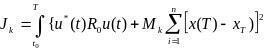
\includegraphics[width=0.8\textwidth]{assets/150}
	\caption*{}
\end{figure}

The problem can be reformulated as follows: for a given value of the
parameter \emph{k}, find the optimal control minimizing the functional
\(J_{k}\)\hspace{0pt} subject to constraints (5)-(7). This problem
belongs to the class of optimal control problems with a free right
boundary and control constraints.

For it, we will construct the Hamiltonian function:

\[H_{k} = u^{*}(t)R_{0}u(t) + (g(x,t) + Bu(t))^{*}\psi_{k}\]

The following solution algorithm is proposed:

Step 1: Let \(k = 0\) .

Step 2: Calculate the optimal control for the k-th iteration using
equation (12), where \(ᴪ_{k}\) is the solution to the conjugate system
of differential equations (11), with the boundary condition at the end:

\begin{longtable}[]{@{}
  >{\raggedright\arraybackslash}p{(\columnwidth - 2\tabcolsep) * \real{0.9333}}
  >{\raggedright\arraybackslash}p{(\columnwidth - 2\tabcolsep) * \real{0.0667}}@{}}
\toprule\noalign{}
\begin{minipage}[b]{\linewidth}\raggedright
\[\Psi_{k}(T) = 2M_{k}\sum_{i = 1}^{n}{\lbrack x_{k}(T) - x_{T}\rbrack}\]
\end{minipage} & \begin{minipage}[b]{\linewidth}\raggedright
(13)
\end{minipage} \\
\midrule\noalign{}
\endhead
\bottomrule\noalign{}
\endlastfoot
\end{longtable}

and \(x_{k}\) is the solution of the original system (4) with initial
conditions (6).

Step 3: Calculate the value of the functional \(J_{k}\) for the obtained
\(x_{k}\) and \(u_{k}\).

Step 4: If \(\left| J_{k} - J_{k - 1} \right| \leq \varepsilon\) proceed
to step 5, otherwise, set \(k = k + 1\) and go back to step 2. (Here,
\(\varepsilon > 0\) is the required accuracy of the calculation).

Step 5: The found pair (\(x_{k}\), \(u_{k}\)) is the optimal solution.

To automate the process of finding the optimal control, a program
"Optim\_Upr.m" was written in MATLAB. As a result of its execution, we
obtain the analytical form of the original and conjugate systems of
differential equations, the form of the Hamiltonian function for the UAV
mathematical model (1)-(3):

H=10.*ux\^{}2+10.*uy\^{}2+(9.80*ux-9.80*sin(O))*fi1+(5.15*uy-9.80*cos(O))/V*fi2-8.34*uy/V/cos(O)*fi3+V*cos(O)*cos(K)*fi4+V*sin(O)*fi5-1.*V*cos(O)*sin(K)*fi6

f1=9.80*ux-9.80*sin(O)

f2=(5.15*uy-9.80*cos(O))/V

f3=-8.34*uy/V/cos(O)

f4=V*cos(O)*cos(K)

f5=V*sin(O)

f6=-1.*V*cos(O)*sin(K)

fp1=(5.15*uy-9.80*cos(O))/V\^{}2*fi2-8.34*uy/V\^{}2/cos(O)*fi3-1.*cos(O)*cos(K)*fi4-1.*sin(O)*fi5+cos(O)*sin(K)*fi6

fp2=9.80*cos(O)*fi1-9.80*sin(O)/V*fi2+8.34*uy/V/cos(O)\^{}2*fi3*sin(O)+V*sin(O)*cos(K)*fi4-1.*V*cos(O)*fi5-1.*V*sin(O)*sin(K)*fi6

fp3=V*cos(O)*sin(K)*fi4+V*cos(O)*cos(K)*fi6

fp4=0

fp5=0

fp6=0

H1=-20.*ux-9.80*fi1

H2=-20.*uy-5.15/V*fi2+8.34/V/cos(O)*fi3

Here f1,\ldots,f6 is the view of the right side of the initial system of
differential equations, fp1,\ldots,fp6 is the view of the right side of
the conjugate system.

The obtained results are transferred to a program written in Delphi,
which performs numerical calculations to find the optimal control.

The results of the program are output to the file "rez.txt," a fragment
of which is provided below:

T=1,00 nt=1000

-10,00\textless=U1\textless=10,00

-5,00\textless=U2\textless=5,00

x0 = 8,00; = 1,00; = 3,00; = 5,00; = 1,00; = 3,00;

xk = 4,00; = 0,50; = 1,50; = 2,50; = 0,50; = 1,50;

F1 == 1009,53 11276,69 11276,69

F2 == 1164,04 20148,99 10102,31

F3 == 1191,48 40409,25 10874,49

F4 == 1127,07 42853,26 5356,66

F5 == 1250,00 184817,12 4551,07

F6 == 1244,47 321606,47 3050,20

A total of 6 functionals F1,\ldots,F6. were calculated. As can be seen
from the last column, the difference between the specified and final
points decreases.

{\bfseries Results and Discussion}. Constructing the conjugate system of
differential equations (11) for the original nonlinear system (1) is a
rather labor-intensive process, especially when the dimensionality
\emph{n} increases, and is practically impossible for \emph{n}
\textgreater{} 3. Furthermore, when forming the Hamiltonian function,
there is often a "human factor" involved, which does not guarantee the
correctness of the analytical calculations. Therefore, the automation of
verifying the conditions of the theorems becomes relevant.

To address this issue, it is recommended to use computer algebra systems
(CAS), such as MATLAB {[}8-9{]}. These systems provide a wide range of
tools for working with algebraic expressions, from simple operations
like calculation and differentiation to more complex ones like series
expansion and integration. The application of such systems is relevant
in various industries, including the aerospace industry.

Numerical calculations showed correspondence with experimental data. The
results are also saved in text files, allowing the visualization of UAV
dynamics in the form of one-dimensional graphs using MATLAB, for which a
special program was developed. Based on the presented theory, an
application was created {[}10{]}.

{\bfseries Conclusions.} The development of unmanned aviation requires the
creation of optimal control methods for dynamic systems, which is
crucial for enhancing the efficiency of unmanned aerial vehicle (UAV)
management. This study confirms the necessity of finding optimal
solutions in the presence of nonlinear equations and control
constraints.

The article proposes a mathematical model of UAV dynamics described by a
system of nonlinear differential equations. Several variants of the
optimal control problem were solved with fixed and variable boundaries,
as well as by using penalty functions and the gradient method to find
optimal trajectories. The solution to the optimal control problem
involves minimizing a functional under given constraints, which requires
significant mathematical computations.

The application of a computer algebra system (MATLAB) enabled the
automation of complex differential equation system calculations and
minimized the human factor, which is important for increasing the
accuracy of computations. Numerical calculations confirmed the
correctness of the proposed theoretical model. The results showed
consistency between calculated data and real experimental observations,
indicating the applicability of the model for real UAV control systems.

The developed "Optim\_Upr.m" program in MATLAB, along with the
application created for visualizing the results, simplifies solving UAV
dynamics control tasks and provides results in the form of text files
and graphs. This opens up opportunities for the further application of
these methods in real-world conditions.

The continued use and development of the proposed algorithms and
software can significantly improve the efficiency of UAV control
systems, enabling them to adapt to changing real-time conditions and be
applied in various industries, including the aviation and space sectors.

\emph{{\bfseries Financing:} The The work was carried out with the support
of the Research Institute of Mathematics and Mechanics at Al-Farabi
Kazakh National University and grant funding for scientific research for
2023--2025 under project AP19678157.}

{\bfseries References}

1.Loginov A.A., Hvan A.A. Aktual\textquotesingle nost\textquotesingle{}
ispol\textquotesingle zovanija bespilotnyh letatel\textquotesingle nyh
apparatov// Aktual\textquotesingle nye problemy aviacii i kosmonavtiki.
-- 2015.-T.1.- S.704 -705.{[}in Russ.{]}

2. Husnutdinov T.D., Shherbakova A.V., Komarova P.A., Rublevskaja E.V.,
Reshetnikov A.Ju. Perspektivy ispol\textquotesingle zovanija bespilotnyh
letatel\textquotesingle nyh apparatov v innovacionnyh proektah//
Aktual\textquotesingle nye problemy aviacii i kosmonavtiki.- 2017.-
T.3.- S.139-141. {[}in Russ.{]}

3.Lju Sh., Li., Tan C., Vu Sh., God\textquotesingle e Zh.-L. Razrabotka
bespilotnyh transportnyh sredstv.- M.:DMK Press.- 2022.-246 s. ISBN
978-5-97060-969-9. {[}in Russ.{]}

4.Avgustov L.I i dr. Navigacija letatel\textquotesingle nyh apparatov v
okolozemnom prostranstve. -- M.: OOO «Nauchtehlitizdat», 2015. -592s.
ISBN 978-5-93728-146-3. {[}in Russ.{]}

5.Berns V.A., Dolgopolov A.V. i dr. Jeksperimental\textquotesingle nyj
modal\textquotesingle nyj analiz letatel\textquotesingle nyh apparatov.
-- Novosibirsk: NGTU, 2023. -- 328 s. ISBN 978-5-7782-3209-9{[}in
Russ.{]}

6.Tang Than\textquotesingle{} Lam Sistemnyj analiz i optimizacija
rezhimov poleta dlja upravlenija letatel\textquotesingle nym apparatom
// Avtoref. disser. kand. tehn. nauk, spec. 05.13.01, Moskva, 2015. --
155 s. {[}in Russ.{]}

7. Mazakova A., Jomartova Sh.,Vfzakov T., Shormanov., Amirkhanov B.
Controllability of an unmanned aerial vehicle.// 2022 IEEE 7th
International Energy Conference (ENERGYCON) - C.1-5.
DOI~10.1109/ENERGYCON53164.2022.9830244

8.Smolencev N.K. MatLAb. Programmirovanie na Visual C\#, Borland
JBuilder, VBA. -- M.: DMK Press, 2009. -- 464s.

9.D\textquotesingle jakonov V., Abramenkova I. MATLAB. Obrabotka
signalov i izobrazhenij. Special\textquotesingle nyj spravochnik. --
SPb.: Piter, 2002. - 608 s. ISBN 5-318-00667-1.

10. A.C. № 45572 ot 05.10.2024. Mazakova A.T., Dzhomartova S.A., Mazakov
T.Ja. Opredelenie optimal\textquotesingle nogo upravlenija BPLA.
Komp\textquotesingle juternaja programma

\emph{{\bfseries Information about the authors}}

Mazakova A.T. - PhD student of the Al-Farabi Kazakh National University,
Almaty, Kazakhstan, e-mail: aigerym97@mail.ru;

Jomartova Sh.A. - Doctor of Technical Sciences, Associate Professor,
Al-Farabi Kazakh National University, Almaty, Kazakhstan, e-mail:
jomartova@mail.ru;

Mazakov T.Zh. -- Doctor of Physical and mathematical sciences,
professor, Al-Farabi Kazakh National University, Almaty, Kazakhstan,
e-mail: tmazakov@mail.ru;

Tokenov G.Ch. - Candidate of Physical and Mathematical Sciences,
Associate Professor, Kazakh National Women\textquotesingle s Pedagogical
University, Almaty, Kazakhstan, e-mail: gumyrbektoike@mail.ru;

Aliaskar M.S. - Lecturer at the International University of Engineering
and Technology, Almaty, Kazakhstan, e-mail: m.alyasqar@gmail.ru

\emph{{\bfseries Сведение об авторах}}

Мазақова А.Т. -- докторант Казахского национального университета
им.аль-Фараби, e-mail: aigerym97@mail.ru;

Джомартова Ш.А. - доктор технических наук, доцент, Казахский
национальный университет им. аль-Фараби, Алматы, Казахстан, e-mail:
jomartova@mail.ru;

Мазаков Т.Ж. -- доктор физико-математических наук, профессор, Казахский
национальный университетим. аль-Фараби, Алматы, Казахстан, e-mail:
tmazakov@mail.ru;

Тойкенов Г.Ч. - кандидат физико-математических наук, доцент, Казахский
национальный женский педагогический университет, Алматы, Казахстан,
e-mail: gumyrbektoike@mail.ru;

Әлиасқар М.С. - докторант Казахского национального университета
им.аль-Фараби, Алматы, Казахстан, e-mail: m.alyasqar@gmail.ru\newpage
{\bfseries IRSTI 44.01.77}

{\bfseries ANALYSIS OF REAL-WORLD AND SIMULATION MODELS AND ALGORITHMS FOR
DETECTING ATTACKS IN WIRELESS SENSOR NETWORKS}

{\bfseries \textsuperscript{1,2}Y. Mardenov\textsuperscript{🖂} ,
\textsuperscript{3}Zh. Iztaev, \textsuperscript{3}Hu Wen-Tsen,
\textsuperscript{1,2}D. Mardenova, \textsuperscript{1,2}D. Baumuratova}

\textsuperscript{1}International Science Complex "Astana", Astana,
Kazakhstan,

\textsuperscript{2}Astana International University, Astana, Kazakhstan,

\textsuperscript{3}M.Auezov South Kazakhstan State University, Shymkent,
Kazakhstan

{\bfseries \textsuperscript{🖂}}Корреспондент-автор: emardenov@gmail.com

Presented are real-world and simulation models, methods, and tools for
simulating attacks on Wireless Sensor Networks (WSNs) intended for use
in network vulnerability research. A comparative analysis was conducted
to identify their advantages and disadvantages. The research
demonstrated that integrating real-world and simulation approaches
contributes to increased accuracy and reliability in attack detection.
Recommendations are proposed for developing flexible and scalable
simulation models, improving the efficiency of attack detection
algorithms, and regularly updating models in accordance with changing
WSN operating conditions and emerging threats.

{\bfseries Key words:} WSN, Real-world models, Simulation models, WSN
attack detection, Attack detection algorithms, Comparative analysis of
detection tools, Integration of detection methods, Network security.

{\bfseries АНАЛИЗ НАТУРНЫХ И ИМИТАЦИОННЫХ МОДЕЛЕЙ И АЛГОРИТМОВ}

{\bfseries ВЫЯВЛЕНИЯ АТАК БСС}

{\bfseries \textsuperscript{1,2}Е. Марденов\textsuperscript{🖂},
\textsuperscript{3}Ж. Изтаев, \textsuperscript{3}Ху Вен-Цен,
\textsuperscript{1,2}Д. Марденова, \textsuperscript{1,2}Д. Баумуратова}

\textsuperscript{1}Международный научный комплекс «Астана», Астана,
Казахстан,

\textsuperscript{2}Международный университет «Астана», Астана,
Казахстан,

\textsuperscript{3} Южно-Казахстанский государственный университет имени
М. Ауэзова, Шымкент, Казахстан,

е-mail: emardenov@gmail.com

В данной статье представлен анализ натурных и имитационных моделей и
алгоритмов выявления атак на беспроводные сенсорные сети (БСС). Описаны
разработанные натурные и имитационные модели, методы и инструменты для
имитации атак, а также результаты экспериментальных исследований.
Сравнительный анализ выявляет преимущества и недостатки каждого подхода,
подчеркивая необходимость интеграции натурных и имитационных методов для
достижения наибольшей точности и надежности в обнаружении атак. В статье
предложены рекомендации по развитию гибких и масштабируемых имитационных
моделей, улучшению алгоритмов обнаружения атак и регулярному обновлению
моделей в соответствии с изменяющимися условиями и угрозами. Результаты
исследования подчеркивают важность комбинированного использования
натурных и имитационных подходов для повышения уровня безопасности БСС.

{\bfseries Ключевые слова:} Беспроводные сенсорные сети (БСС), Натурные
модели, Имитационные модели, Выявление атак, Алгоритмы обнаружения,
Сравнительный анализ, Интеграция методов, Безопасность сетей

{\bfseries СЫМСЫЗ СЕНСОРЛЫҚ ЖЕЛІЛЕРДІҢ ТАБИҒИ ЖӘНЕ СИМУЛЯЦИЯЛЫҚ МОДЕЛЬДЕР
МЕН ШАРУАЛДАРДЫ АНЫҚТАУ АЛГОРИТМДЕРІН ТАЛДАУ}

{\bfseries \textsuperscript{1,2}Е. Марденов\textsuperscript{🖂},
\textsuperscript{3}Ж. Изтаев, \textsuperscript{3}Ху Вэн-Цен,
\textsuperscript{1,2}Д. Марденова, \textsuperscript{1,2}Д. Баумуратова}

\textsuperscript{1} «Астана» халықаралық ғылыми кешені, Астана,
Қазақстан,

\textsuperscript{2}Астана халықаралық университеті, Астана, Қазақстан,

\textsuperscript{3} М.Әуезов атындағы Оңтүстік Қазақстан мемлекеттік
университеті, Шымкент, Қазақстан,

е-mail: emardenov@gmail.com

Бұл мақалада сымсыз сенсорлық желілерге шабуылдарды анықтаудың табиғи
және имитациялық модельдері мен алгоритмдерін талдау ұсынылған.
Әзірленген табиғи және имитациялық модельдер, шабуылдарды модельдеу
әдістері мен құралдары және эксперименттік зерттеулердің нәтижелері
сипатталған. Салыстырмалы талдау шабуылдарды анықтауда ең жоғары дәлдік
пен сенімділікке қол жеткізу үшін табиғи және имитациялық әдістерді
біріктіру қажеттілігін көрсете отырып, әрбір тәсілдің артықшылықтары мен
кемшіліктерін анықтайды. Мақалада икемді және масштабталатын модельдеу
модельдерін дамыту, шабуылдарды анықтау алгоритмдерін жақсарту және
өзгеретін жағдайлар мен қауіптерге сәйкес модельдерді үнемі жаңарту
бойынша ұсыныстар берілген. Зерттеу нәтижелері қауіпсіздік деңгейін
жақсарту үшін табиғи және имитациялық тәсілдерді біріктіріп қолданудың
маңыздылығын көрсетеді сымсыз сенсорлық желілер.

{\bfseries Түйін сөздер:} Сымсыз сенсорлық желілер, табиғи модельдер,
модельдеу модельдері, шабуылдарды анықтау, анықтау алгоритмдері,
салыстырмалы талдау, әдістерді біріктіру, желі қауіпсіздігі

{\bfseries Introduction.} Wireless Sensor Networks (WSNs) are widely and
comprehensively utilized, playing a crucial role in addressing various
practical tasks in military, industrial, and domestic spheres. WSNs
represent a multifunctional communication foundation of cyber-physical
systems with artificial intelligence elements, providing connectivity
between various sensor devices and systems that can collect, process,
and transmit environmental data in real-time. This foundation enables
effective automatic monitoring and control of various processes and
objects over extensive and hard-to-reach areas {[}1, 2{]}.

However, the use of WSNs is associated with certain risks due to their
security vulnerabilities. Attacks by malicious actors on such networks
can lead to serious consequences, including data interception,
tampering, and disruption of the functionality of technical equipment,
particularly sensor devices that are fundamental elements of WSNs.
Consequently, there is increasing importance in developing effective
measures to counter potential threats within WSN security frameworks.

A critical measure to combat these threats is the development of
efficient methods for detecting, recognizing, and preventing network
attacks. Specifically, analytical and simulation models of attacker
actions on WSNs allow for the study of processes within WSNs induced by
these attacks. Such models are based on mathematical and statistical
descriptions of attacker and defender behaviors using real network data,
parameters, and characteristics. They enable the creation of virtual
environments for comprehensive simulation of WSNs, including the
operation of sensor nodes, communication processes between nodes over
radio channels, data reception and transmission, and routing {[}1, 3,
4{]}.

This study aims to conduct testing and comparative analysis of natural
and simulation models of attacks on WSNs, attack detection algorithms,
and to develop recommendations for their effective implementation.

{\bfseries Materials and methods.} \emph{Analytical review of literary
sources on the research issue.}

There are several different types of attacks that can occur in WSNs.

Threats to confidentiality involve interception and observation, where
attackers intercept data or analyze traffic to obtain confidential
information. Threats to integrity are associated with data modification,
source impersonation, message replay, and message denial, which lead to
data distortion and incorrect network operation. Attackers can alter
messages, spoof sources, replay intercepted data, or deny
sending/receiving messages. Availability threats aim to disrupt message
delivery, causing network service denial. These attacks include Denial
of Service (DoS), node capture, and resource depletion attacks, leading
to node overload or network disconnection. Such attacks can severely
disrupt network operation, highlighting the importance of protecting
against them. {[}2, 4, 5{]}

The paper presents {[}6{]} a new intrusion detection model for WSNs
using fuzzy neural networks and feedforward neural networks.
Experimental results show that the proposed model achieves detection
rates averaging 97.8\% with maximum detection accuracy of 98.8\%.
Evaluations were compared against benchmark models based on support
vector machines (SVM), decision trees (DT), and random forest (RF)
models.

Authors {[}7{]} introduced detection of multiple attacks in wireless
sensor networks using artificial neural networks. The dataset is split
into training and testing using a multi-layer perceptron artificial
neural network to detect ten classes of attacks, including DoS attacks.
Research using benchmark datasets UNSW-NB, WSN-DS, NSL-KDD, and
CICIDS2018 showed that the proposed system achieves an average detection

In article {[}8{]}, the use of spatial information for detecting and
localizing multiple attacks across single and multiple nodes is
presented. A scalable and energy-efficient anomaly detection mechanism
based on clusters (SEECAD) is described for detecting DoS attacks
without key management schemes to enhance network lifespan. Detection
speed, false alarm rate, packet delivery ratio, overhead costs, energy
consumption, and average packet delay are various performance metrics
used to evaluate network performance.

In {[}9{]}, an enhanced high-performance secure routing protocol based
on clustering is proposed. A key feature of this protocol is its
consideration of aspects such as energy consumption, packet reduction,
congestion management, encrypted data transmission, and monitoring of
malicious nodes to improve data management quality. To demonstrate the
feasibility of the proposed method, performance metrics such as
ransomware attack detection level, ergodic residual energy per round,
early clone attack detection, throughput maximization, delay, maximum
throughput, and network lifespan maximization were used.

The works {[}10{]} conducted modeling to demonstrate that the proposed
EdDSA-XOR functionality reduces time and energy costs by 0.13\% and
0.07\% respectively, compared to other methods. Node authentication in
the network was tested against "man-in-the-middle" attacks.

The paper proposes {[}11{]} an effective method for detecting black hole
and Sybil attacks using the Adaptive Taylor Sail (Adaptive Taylor-SFO)
algorithm. The BSS nodes are modeled in the network, followed by routing
using Adaptive Taylor-SFO. The router was developed by integrating the
Adaptive concept with the Taylor series and the Sail Fish optimizer
(SFO) to select the optimal route considering adaptability metrics such
as delay, energy, and distance. Black hole and Sybil attack detection is
performed by the Deep stacked automatic encoder. Thus, the proposed
system effectively classifies normal, black hole, and Sybil attacks. The
analysis of the reviewed works made it possible to determine the most
common types of attacks on WSNs (Table 1), the mechanisms of their
impact, possible consequences and methods of mitigating the
consequences.

{\bfseries Table 1 - Most common attacks on WSN}

\begin{longtable}[]{@{}
  >{\raggedright\arraybackslash}p{(\columnwidth - 8\tabcolsep) * \real{0.0723}}
  >{\raggedright\arraybackslash}p{(\columnwidth - 8\tabcolsep) * \real{0.1910}}
  >{\raggedright\arraybackslash}p{(\columnwidth - 8\tabcolsep) * \real{0.3046}}
  >{\raggedright\arraybackslash}p{(\columnwidth - 8\tabcolsep) * \real{0.2203}}
  >{\raggedright\arraybackslash}p{(\columnwidth - 8\tabcolsep) * \real{0.2117}}@{}}
\toprule\noalign{}
\endhead
\bottomrule\noalign{}
\endlastfoot
№ & Attack name & Mechanism of action & Consequences & Mitigation
Strategies \\
1 & Routing attack {[}6{]} & Routing attacks involve manipulating
routing mechanisms to redirect or block data flows. Attackers exploit
vulnerabilities across various layers of the network protocol stack.
Examples include black hole attacks, where malicious nodes discard
received data, and wormhole attacks, where attackers create shortcuts
between remote nodes. & Data loss. Network segmentation. Resource
exhaustion. & Secure routing protocols. Anomaly detection. Cooperative
verification. Hop count verification. Location verification. \\
& The man in the middle attack {[}10{]} & Man-in-the-middle attack
involves an attacker secretly intercepting and relaying messages between
two communicating nodes without their knowledge. The attacker can
manipulate the contents of the messages or simply eavesdrop on them.
Man-in-the-middle attacks exploit the absence of secure communication
channels and can occur at various protocol levels, including
application, transport, and network layers. & Data falsification:
Unauthorized access leading to breach of confidentiality. & Encryption.
Public Key Infrastructure (PKI). Certificate revocation. Timestamps and
one-time passwords. Intrusion detection systems. \\
& Sibyl {[}12{]} & Sybil attack involves creating a network of malicious
nodes that impersonate legitimate nodes. The attacker\textquotesingle s
goal is to inject false information or disrupt network communication.
These attacks can undermine data accuracy, routing efficiency, and
overall network functionality. & Data integrity

Routing manipulation

Resource exhaustion & Behavioral analysis

Trust-based systems

Physical layer measurements

Reputation mechanisms

Cryptographic methods \\
& Eavesdropping {[}13{]} & In an eavesdropping attack, an attacker is
placed within the range of two or more sensor nodes using the
transmission of unencrypted or weakly encrypted data. The attacker
passively intercepts data packets without changing the functionality of
the network. Eavesdropping can occur at various levels of the
communications stack, from the physical layer to the application layer.
& - Data confidentiality

- Data integrity

- Network mapping & - - Encryption

- Secure key exchange

- Frequency hopping

- Intrusion detection

- Secure protocols \\
& Denial of Service (DoS)

{[}14,15{]} & A DoS attack exploits vulnerabilities in WSNs to reduce
their performance or even disable them. Attackers employ various methods
such as flooding the network with excessive traffic or exploiting
protocol vulnerabilities. In the context of WSNs, attacks can target
nodes, communication channels, or the sink node responsible for
aggregating data. & Data loss

Resource depletion

Network partitioning

Delayed responses & Intrusion detection

Rate limiting

Traffic filtering

Energy consumption management

Collaborative defense \\
\end{longtable}

\emph{Empirical models and attack detection algorithms.}

\emph{Description of the empirical models used for attack detection}

Natural models for detecting attacks in WSNs involve physically
implemented networks where nodes and sensors are deployed in real
operational conditions. These models utilize real devices such as
microcontrollers, radio modules, and sensors that interact within
realistic environmental settings. The primary advantage of natural
models lies in their ability to accurately reproduce real network
operation scenarios, including potential external interferences and
physical attacks.

Research on natural models for attack detection in wireless sensor
networks includes functional and quantitative characteristics. Attack
detection methods are categorized into signature-based, anomaly-based,
and hybrid approaches, covering attacks on availability,
confidentiality, integrity, and authentication. Hardware and network
characteristics of sensors and nodes, data processing algorithms, and
monitoring systems play a crucial role. Quantitative metrics include
detection accuracy, detection time, energy consumption, throughput,
delay, and scalability.

For instance, platforms like TinyOS and Contiki are used to test
intrusion detection systems, achieving 95\% accuracy with low false
positive rates. Machine learning-based systems such as K-means and SVM
can achieve classification accuracies up to 98\%. Distributed detection
methods include autonomous algorithms that depend on node density and
algorithm complexity {[}15, 16{]}. Table 2 presents empirical
experiments on attack detection and their outcomes.

{\bfseries Table 2 - Full-scale experiments to detect attacks and their
results}

\begin{longtable}[]{@{}
  >{\raggedright\arraybackslash}p{(\columnwidth - 6\tabcolsep) * \real{0.0923}}
  >{\raggedright\arraybackslash}p{(\columnwidth - 6\tabcolsep) * \real{0.1915}}
  >{\raggedright\arraybackslash}p{(\columnwidth - 6\tabcolsep) * \real{0.3709}}
  >{\raggedright\arraybackslash}p{(\columnwidth - 6\tabcolsep) * \real{0.3453}}@{}}
\toprule\noalign{}
\endhead
\bottomrule\noalign{}
\endlastfoot
№ & Name & Description & Results \\
1. & jamming attack & Nodes of the network were deployed in an open
space with various obstacles. A jamming attack was initiated using a
powerful radio transmitter, creating interference within a specific
frequency range. & It was found that the jamming attack significantly
reduces signal strength and increases packet loss frequency. The
detection system was able to identify the attack based on signal
strength and packet loss analysis, achieving a detection accuracy of
92\%. \\
2. & resource exhaustion attack & Nodes in the experiment were
programmed to perform energy-intensive tasks. The attacker sent a large
number of false requests to the nodes to accelerate their battery
discharge. & Nodes with depleted resources ceased normal operation. The
detection model based on energy consumption monitoring successfully
identified the attack with 87\% accuracy, enabling timely network
protection measures to be implemented. \\
3. & replay attack & The experiment involved nodes equipped with
built-in authentication mechanisms. The attacker retransmitted
previously intercepted legitimate messages. & The detection system based
on timestamps and authentication algorithms successfully identified
repeated messages with 95\% accuracy, preventing the execution of false
commands. \\
\end{longtable}

The effectiveness of full-scale models and attack detection algorithms
is assessed based on several key parameters (Table 3)

{\bfseries Table 3 - Evaluation of the effectiveness of full-scale models
and algorithms}

\begin{longtable}[]{@{}
  >{\raggedright\arraybackslash}p{(\columnwidth - 2\tabcolsep) * \real{0.5000}}
  >{\raggedright\arraybackslash}p{(\columnwidth - 2\tabcolsep) * \real{0.5000}}@{}}
\toprule\noalign{}
\endhead
\bottomrule\noalign{}
\endlastfoot
{\bfseries accuracy} & {\bfseries detection time} \\
The ability of the model to correctly identify attacks and minimize
false positives was evaluated in the conducted experiments. Accuracy
ranged from 87\% to 95\%, depending on the type of attack and the
algorithm applied. & The time required to identify an attack after its
onset. Natural models demonstrated the ability to detect attacks in real
time, which is critical for preventing damage. \\
{\bfseries resource consumption} & {\bfseries adaptability} \\
The volume of computational and energy resources required for algorithm
operation. Efficient algorithms minimize resource consumption, which is
particularly crucial for sensor nodes with limited batteries. & The
ability of the model and algorithms to adapt to changes in the
environment and new types of attacks. Natural models have demonstrated
good adaptability when new nodes are added or when the network topology
changes. \\
\end{longtable}

Thus, natural models and intrusion detection algorithms in WLANs are
effective tools for studying and protecting networks, ensuring high
accuracy and timely detection of attacks in real operational conditions.

\emph{Imitative models and intrusion detection algorithms}

Description of Developed Simulation Models. Simulation models are
software tools designed to replicate the operations of Wireless Sensor
Networks (WSNs) and simulate various attack scenarios in a controlled
environment. Within the scope of the conducted research, simulation
models were tested that accurately reproduce the behavior of sensor
nodes, communication protocols, and interactions with the external
environment. These models are based on the following principles:

1. Multi-layered architecture of the model: The simulation model
includes physical, data link, network, and application layers, enabling
detailed reproduction of all aspects of Wireless Sensor Network (WSN)
operation.

2. Network topology modeling: Supports various topologies such as mesh,
star, and tree, allowing exploration of how topology affects resilience
to attacks.

3. Parameter flexibility: The model allows configuration of node
parameters such as transmitter power, data transmission rate, and energy
consumption, crucial for investigating different attack scenarios.

All simulation models are built using diverse mathematical and
computational methods. These models facilitate testing and analyzing
network behavior under attack, evaluating detection accuracy, and
justifying the realism of simulated conditions (Table-4).

{\bfseries Table 4 - Composition and structure of models}

\begin{longtable}[]{@{}
  >{\raggedright\arraybackslash}p{(\columnwidth - 6\tabcolsep) * \real{0.0752}}
  >{\raggedright\arraybackslash}p{(\columnwidth - 6\tabcolsep) * \real{0.1812}}
  >{\raggedright\arraybackslash}p{(\columnwidth - 6\tabcolsep) * \real{0.3248}}
  >{\raggedright\arraybackslash}p{(\columnwidth - 6\tabcolsep) * \real{0.4188}}@{}}
\toprule\noalign{}
\endhead
\bottomrule\noalign{}
\endlastfoot
№ & Model & Composition and structure of models & Mathematical
description \\
1 & Network layer & \emph{Graph model: Sensors and nodes are represented
as a graph} 𝐺 ( 𝑉 , 𝐸 ) G(V,E), where 𝑉 V - a set of vertices (nodes),
and 𝐸 E - many edges (communication channels).

\emph{Topology:} The parameters of the network topology are defined,
including the distance between nodes, node density, and network type
(e.g., star, tree, mesh network). &
\emph{G}(\emph{V},\emph{E})=\{(\emph{v\textsubscript{i}}\textsubscript{\hspace{0pt}},\emph{v\textsubscript{j}}\hspace{0pt})
∣
\emph{v\textsubscript{i}}\hspace{0pt},\emph{v\textsubscript{j}}\hspace{0pt}∈\emph{V},
\emph{e\textsubscript{ij}}\hspace{0pt}∈\emph{E}\} (1)

Где

𝑉=\{𝑣\textsubscript{1},𝑣\textsubscript{2},\ldots,𝑣\textsubscript{𝑛}\} -
many nodes,

𝐸=\{𝑒\textsubscript{𝑖𝑗}\} E=\{e\textsubscript{ij}\} - many communication
channels. \\
2 & Traffic model & \emph{Data flow:} The distribution of traffic
between nodes is described. This is achieved using probabilistic models
such as Poisson distribution or Markov models. &
\emph{λij}\hspace{0pt}=Rate(\emph{vi}\hspace{0pt}→\emph{vj}\hspace{0pt})
(2)

where

𝜆\textsubscript{𝑖𝑗} - traffic intensity between nodes
𝑣\textsubscript{𝑖}\hspace{0pt} and 𝑣\textsubscript{𝑗}\hspace{0pt}, which
may follow a Poisson distribution:

(3) \\
3 & Attack model & \emph{Types of attacks:} Models are defined for
various types of attacks, such as

DoS attacks, data interception attacks, and data integrity attacks.

\emph{Attacker behavior:} The strategy of the attacker is determined,
including the frequency and intensity of attacks. & (4)

where

𝑑 - distance to target,

𝜃 - interception angle. \\
4 & Detection model & \emph{Methods:} Implementation includes detection
algorithms such as signature-based, anomaly-based, and hybrid methods.

\emph{Machine} learning algorithms: Utilized for traffic classification,
such as K-means, SVM, neural networks. & Anomalous method:

(5)

where

𝑥\textsubscript{𝑖} x\textsubscript{i} \hspace{0pt} - measured value,

μ\textsubscript{i} \hspace{0pt} - average value,

𝑤\textsubscript{𝑖} \hspace{0pt} - weight coefficient.

Machine learning algorithms: K-means:

(5)

Гwhereде

𝐽 - loss function,

𝑘 - number of clusters,

𝑥 \textsubscript{𝑗}\textsuperscript{( 𝑖 )} \hspace{0pt} - data points,

𝜇\textsubscript{𝑖} \hspace{0pt} - cluster centroids \\
\end{longtable}

Model adequacy assessment involves comparing simulation results with
real-world data, including topology parameters, traffic intensity, and
attack frequency. A model is considered adequate if its behavior does
not statistically differ from real data, often verified using tests like
the Kolmogorov-Smirnov test. An example application of such models could
include testing intrusion detection systems on the TinyOS platform,
achieving a detection accuracy of 95\% with a false positive rate of
less than 2\%, utilizing a hybrid approach to enhance accuracy and
minimize energy consumption.

\emph{Methods and tools for simulating attacks on wireless sensor
networks}

For implementing simulation models, a number of modern tools and methods
were utilized to ensure high accuracy and scalability of the research.
The key tools include:

1. NS-3 (Network Simulator 3): A powerful tool for network simulation
that allows reproduction of a wide range of protocols and attack
scenarios on WLANs. NS-3 provides detailed modeling of node behavior and
interactions between nodes.

2. MATLAB/Simulink: Used for mathematical modeling and analysis of
attack detection algorithms. MATLAB facilitates the development and
testing of complex algorithms, as well as the analysis of data obtained
from simulations.

3. Omnet++: A tool for modeling and simulating networks, offering high
flexibility in network parameter configuration and attack scenarios.
Omnet++ supports extensibility, enabling integration of custom models
and algorithms.

These tools collectively support comprehensive modeling, simulation, and
analysis of wireless sensor networks (WSNs), enabling researchers to
evaluate the performance and effectiveness of various security
mechanisms against different types of attacks.

{\bfseries Results and discussion.} Results of simulation experiments and
their analysis. Within the

framework of conducted simulation experiments, various types of attacks
on WLANs were simulated, including jamming attacks, resource exhaustion
attacks, replay attacks, and spoofing attacks. The results of the
experiments enabled a detailed analysis of the effectiveness of the
proposed models and attack detection algorithms (Table 5).

{\bfseries Table 5 - Composition and structure of models}

\begin{longtable}[]{@{}
  >{\raggedright\arraybackslash}p{(\columnwidth - 6\tabcolsep) * \real{0.0475}}
  >{\raggedright\arraybackslash}p{(\columnwidth - 6\tabcolsep) * \real{0.1443}}
  >{\raggedright\arraybackslash}p{(\columnwidth - 6\tabcolsep) * \real{0.5248}}
  >{\raggedright\arraybackslash}p{(\columnwidth - 6\tabcolsep) * \real{0.2835}}@{}}
\toprule\noalign{}
\endhead
\bottomrule\noalign{}
\endlastfoot
№ & Attack & Description of the experiment & Results \\
1. & jamming attack & An experiment to simulate a jamming attack was
conducted using a powerful transmitter in Omnet++, a platform for
modeling network systems. The experiment involved creating a wireless
sensor network of 100 nodes with a random topology and a transmission
radius of 50 meters. The experiment consisted of three stages: network
initialization without attack, introduction of the jamming transmitter,
and data collection. The collected data included received signal
strength indicator (RSSI), packet loss, and transmission delay,
amounting to approximately 10,000 records. Data processing was performed
using statistical methods and machine learning algorithms such as
K-means and SVM. The data processing methodology included data
filtering, analysis of signal strength levels, and anomaly
classification {[}17, 18{]}. & The results showed that the jamming
attack significantly reduces communication quality and increases
latency. Simulation algorithms were able to detect the attack with 94\%
accuracy by analyzing signal strength and packet loss rates. The
experiment demonstrated the possibility of using this technique in real
wireless sensor networks. \\
2. & resource exhaustion attack & A simulation experiment for a resource
exhaustion attack was conducted using the NS-3 network simulator. The
experimental setup included a wireless sensor network comprising 50
nodes, each equipped with a limited battery. The experiment was planned
by creating the network, setting battery parameters, and launching a
series of attacks involving sending a large number of false requests to
the nodes. During the experiment, data on energy consumption, node
response time, and failure rate were collected. Approximately 5000 data
records were gathered, covering all stages of the attack. Data
processing was carried out using an energy consumption monitoring
methodology developed and described in {[}19{]}. This methodology
included data filtering, analysis of energy consumption time series, and
detection of deviations from normal behavior. & Algorithms based on this
methodology were able to identify abnormal behavior with an accuracy of
89\% and an average attack detection time of 2.3 seconds. The
effectiveness of the methodology was confirmed by its high accuracy and
rapid detection of attacks. The experiment demonstrated that the
proposed methodology is effective for application in real-world
conditions of wireless sensor networks. \\
3. & replay attack & Experimental studies aimed at examining replay
attacks were conducted using a model created in the Simulink
environment. In this experiment, the model simulated the repeated
transmission of intercepted messages, mimicking a scenario where an
attacker could re-execute previously executed commands. The experimental
setup consisted of a network model including several nodes and data
transmission mechanisms configured to implement replay attacks. The
experiment planning involved configuring model parameters, defining
attack characteristics, and selecting detection methods.

During the experiment, data related to message timestamps, as well as
parameters of authentication and integrity verification methods, were
collected. The total amount of gathered data was about 2,000 records,
covering various attack scenarios and the system\textquotesingle s
responses to them. The data were processed using algorithms based on
analyzing message timestamps and authentication methods. The data
processing methodology included filtering out repeated messages and
verifying their compliance with expected time intervals {[}19{]}. & The
experimental results showed that algorithms based on timestamps and
authentication methods successfully detected replayed messages with an
accuracy of 97\%, significantly reducing the risk of executing false
commands and enhancing the effectiveness of the replay attack defense
system. \\
4. & spoofing & Experimental studies focused on spoofing attacks were
conducted using Simulink software. The experiment was designed by
creating scenarios in which an attacker sent false messages, pretending
to be legitimate network nodes, with the aim of infiltrating the system.
Parameters of the transmitted messages, such as node identifier, message
content, and timestamp, were recorded for data collection. The total
amount of data collected was approximately 3,000 records, covering
various attack scenarios and network responses. For data analysis,
algorithms for node identity verification and behavior analysis
developed by the experiment\textquotesingle s authors were applied. The
data processing methodology included the identification of anomalous
nodes, comparison of their behavior with samples of normal functioning,
and detection of deviations {[}20{]}. & As a result of the experiment,
the model was able to effectively detect spoofing attacks with 92\%
accuracy. The system\textquotesingle s response time to detect the
attack was 1.8 seconds, demonstrating the high reactivity and efficiency
of the developed algorithms. The obtained results confirm the
effectiveness of the proposed spoofing attack protection methodology and
its readiness for practical application in real network systems. \\
\end{longtable}

Analysis of the results showed that the developed simulation models and
algorithms are highly effective in detecting attacks on WSNs. The
experiments conducted allowed for a detailed study of network behavior
under various types of attacks and proposed algorithms that demonstrate
high accuracy and promptness in detection. The results confirm the
feasibility of using simulation models in the research and development
of protection systems for wireless sensor networks.

\emph{Comparative analysis of full-scale and simulation approaches.}

\emph{Methodology for Comparing Physical and Simulation Models.}

To conduct a comparative analysis of physical and simulation models, the
following methodological steps were developed and applied:

Selection of Representative Attack Scenarios: Typical attack scenarios
were chosen, such as jamming, resource exhaustion attacks, replay
attacks, and spoofing. These scenarios cover a wide range of threats to
wireless sensor networks (WSNs).

Construction of Physical Models: The implementation of physical models
involved deploying sensor nodes in real operational conditions. Various
network topologies, such as mesh and star, were used to ensure a
diversity of conditions. Real devices were subjected to attack impacts
to collect data on network behavior.

Creation of Simulation Models: Simulation models were developed using
tools like NS-3 and Omnet++, allowing for accurate reproduction of the
conditions and behavior of sensor nodes, as well as attack impacts.
These models were configured to match the conditions of the physical
experiments.

Comparison of Physical and Simulation Models: The comparison was
conducted based on several criteria, including attack detection
accuracy, response time, resource consumption, and adaptability to
changes in network conditions (Table 6).

{\bfseries Table 6 - Composition and structure of models}

\begin{longtable}[]{@{}
  >{\raggedright\arraybackslash}p{(\columnwidth - 2\tabcolsep) * \real{0.5009}}
  >{\raggedright\arraybackslash}p{(\columnwidth - 2\tabcolsep) * \real{0.4991}}@{}}
\toprule\noalign{}
\endhead
\bottomrule\noalign{}
\endlastfoot
{\bfseries accuracy} & {\bfseries detection time} \\
The model\textquotesingle s ability to correctly identify attacks and
minimize false positives. Accuracy was measured as the ratio of
correctly detected attacks to the total number of attacks. & The time
required to identify an attack after it has begun. Fast detection is
critical to minimizing the damage from attacks. \\
{\bfseries resource consumption} & {\bfseries adaptability} \\
The amount of computing and energy resources required to run detection
algorithms. This criterion is especially important for WSN nodes with
limited batteries and computing power. & The ability of the model and
algorithms to adapt to changes in network conditions and new types of
attacks. This includes the model\textquotesingle s ability to work
across different network topologies and load changes. \\
\end{longtable}

{\bfseries Table 7 - Results of comparative analysis, identified advantages
and disadvantages of models}

\begin{longtable}[]{@{}
  >{\raggedright\arraybackslash}p{(\columnwidth - 4\tabcolsep) * \real{0.2220}}
  >{\raggedright\arraybackslash}p{(\columnwidth - 4\tabcolsep) * \real{0.3678}}
  >{\raggedright\arraybackslash}p{(\columnwidth - 4\tabcolsep) * \real{0.4102}}@{}}
\toprule\noalign{}
\endhead
\bottomrule\noalign{}
\endlastfoot
& Advantages: & Flaws: \\
Full-scale models & -Highly realistic: Full-scale models accurately
reflect actual operating conditions, including physical disturbances and
unforeseen factors.

-Relevance of data: Data collected in field experiments are direct
results of the operation of real devices and protocols. & - High costs:
Deploying and maintaining full-scale models requires significant
financial and time resources.

-Limited scalability: It is difficult and expensive to scale up field
experiments to large networks or different scenarios. \\
Simulation models & -Flexibility and scalability: Simulation models are
easily customized and scalable for different scenarios and network
topologies.

-Low costs: Simulation experiments are carried out in a software
environment, which significantly reduces costs compared to full-scale
experiments. & - Limited realism: Simulation models may not fully
account for all real-world physical and environmental factors, which may
lead to variations in results.

- Dependence on model accuracy: The effectiveness of simulation models
is highly dependent on the accuracy of reproducing real-world conditions
and network behavior. \\
\end{longtable}

In general, both approaches have their strengths and weaknesses, but
their combination can provide the most complete and reliable analysis of
attacks on WSNs. Full-scale models provide high accuracy and data
relevance, while simulation models offer flexibility and
cost-effectiveness. The optimal solution is to use full-scale
experiments to verify and calibrate simulation models, which allows you
to combine the advantages of both approaches.

{\bfseries Conclusions.} Analysis of full-scale and simulation models and
algorithms for identifying attacks on WSNs shows that both approaches
have their own unique advantages and disadvantages. Full-scale models
provide highly accurate and up-to-date data because they reproduce
real-life network operating conditions. However, their use is associated
with high costs and limited scalability. Simulation models, in contrast,
offer flexibility and cost-effectiveness, allowing easy adjustment of
parameters and scale-up of experiments, but may not fully account for
all real-world physical factors.

Based on the presented data, we can conclude that the combined use of
full-scale and simulation approaches is optimal in the context of
ensuring the security of wireless sensor networks. The integration of
natural and simulation methods makes it possible to jointly use their
advantages, ensuring high accuracy and reliability of attack detection
algorithms. Using field data to calibrate and verify simulation models
plays an important role in achieving high accuracy in network
vulnerability analysis. Recommendations for improving models and
algorithms, including developing flexible and scalable simulation
models, improving attack detection algorithms, and regularly updating
models, are aimed at increasing the effectiveness of the attack
detection system. This combined use of methods and the development of
infrastructure for field experiments seem to be the most effective ways
to improve the security of wireless sensor networks in the face of
rapidly changing threats. This work by the staff of the International
Scientific Complex "Astana" is carried out with the financial support of
the Science Committee of the Ministry of Science and Higher Education of
the Republic of Kazakhstan (Grant No. AP19680345).

{\bfseries References}

1. Lei Zou, Zidong Wang, Bo Shen, Hongli Dong, Guoping Lu, Encrypted
Finite-Horizon Energy-to-Peak State Estimation for Time-Varying Systems
Under Eavesdropping Attacks: Tackling Secrecy Capacity, IEEE/CAA Journal
of Automatica Sinica. -2023. Vol. 10(4).

-P. 985-996. DOI 10.1109/JAS.2023.123393.

2. A. Adamova, T. Zhukabayeva and Y. Mardenov Machine Learning in
Action: An Analysis of its Application for Fault Detection in Wireless
Sensor Networks // 2023 IEEE International Conference on Smart
Information Systems and Technologies (SIST), Astana, Kazakhstan, 2023,
P.506-511. DOI 10.1109/SIST58284.2023.10223548.

3.G.P.S. Kumar, J. R. R. Kumar and S. R. T, Design of Secure
Communication Methodologies for WSN Assisted IoT Applications, 2022 2nd
Asian Conference on Innovation in Technology (ASIANCON), Ravet, India.//
-2022. -P.1-5. DOI 10.1109/ASIANCON55314.2022.9908931.

4. S.A.H. Antar et al. Classification of Energy Saving Techniques for
IoT-based Heterogeneous.Wireless Nodes //Procedia Comput. Sci. -2020.-
Vol.171. - P. 2590-2599

5. Kalaivanan Karunanithy et al. Cluster-tree based energy efficient
data gathering protocol for industrial automation using WSNs and IoT//
J. Indust. In format. Integrat.// -2020.- Vol.19.

DOI 10.1016/j.jii.2020.100156

6. Ezhilarasi, M., Gnanaprasanambikai, L., Kousalya, A. et al. A novel
implementation of routing attack detection scheme by using fuzzy and
feed-forward neural networks //Soft Comput. -2023. Vol. 27.- P.
4157-4168. DOI 10.1007/s00500-022-06915-1

7. J. Panda, and S. Indu Localization and Detection of Multiple Attacks
in Wireless Sensor Networks Using Artificial Neural Network// Wireless
Communications and Mobile Computing.-

-2023.-Vol. 7. - P.1-29. DOI 10.1155/2023/2744706

8. Premkumar, M., Ashokkumar, S.R., Jeevanantham, V. et al. Scalable and
Energy Efficient Cluster Based Anomaly Detection Against Denial of
Service Attacks in Wireless Sensor Networks.// Wireless Pers Commun.
-2023.- Vol.129.- P.2669-2691.

DOI 10.1007/s11277-023-10252-3

9. Roberts M.K., Ramasamy P. An improved high performance clustering
based routing protocol for wireless sensor networks in IoT// Telecommun
Syst. -2023.- Vol. 82.- P. 45-59.

DOI 10.1007/s11235-022-00968-1

10. Yuvaraj, N., Raja, R.A., Karthikeyan, T. et al. Improved
Authentication in Secured Multicast Wireless Sensor Network (MWSN) Using
Opposition Frog Leaping Algorithm to Resist Man-in-Middle Attack//
Wireless Pers Commun. -2022.- Vol. 123. - P. 71715-1731

DOI 10.1007/s11277-021-09209-1

11. M. Kumar and J. Ali, Adaptive Taylor-Sail Fish Optimization based
deep Learning for Detection of Black Hole and Sybil Attack in Wireless
Sensor Network// International Conference on Sustainable Computing and
Data Communication Systems (ICSCDS), Erode, India. -2023. - P.
1237-1244. DOI 10.1109/ICSCDS56580.2023.10104946.

12. Orman, A., Üstün, Y. \& Dener, M. Detailed analysis of sybil attack
in wireless sensor networks // International Journal of Sustainable
Engineering and Technology.-2023.-Vol.7(1)-P.41-54.

https://dergipark.org.tr/en/pub/usmtd/issue/78577/1305047

13. Y. Liu, X. Ma, L. Shu, G. P. Hancke, and A. M. Abu-Mahfouz, From
Industry 4.0 to Agriculture 4.0: current status, enabling technologies,
and research challenges// IEEE Transactions on Industrial Informatics.
-2021.-Vol. 17(6)- P. 4322-4334. DOI 10.1109/TII.2020.3003910

14. A. Williams, P. Suler,J. Vrbka Business process optimization,
cognitive decision-making algorithms, and artificial intelligence
data-driven internet of things systems in sustainable smart
manufacturing//Journal of Self-Governance and Management Economics.
-2020. Vol.8(4).-P. 39-48. DOI 10.22381/JSME8420204

15. Wendi Rabiner Heinzelman, Anantha Chandrakasan,Hari Balakrishnan.
Energy-efficient communication protocol for wireless microsensor
networks//In Proceedings of the 33rd annual Hawaii international
conference on system sciences. -2000. - P. 10.

16. Ibrahim Alrashdi, Ali Alqazzaz, Raed Alharthi, Esam Aloufi, Mohamed
A Zohdy Hua Ming. Fbad: Fog-based attack detection for iot healthcare in
smart cities //In 2019 IEEE 10th Annual Ubiquitous Computing,
Electronics \& Mobile Communication Conference (UEMCON). -2019. --P.
515-522. DOI 10.1109/UEMCON47517.2019.8992963

17. Chen M., Liu W., Zhang, N., Li J., Ren Y., Yi M., Liu A. GPDS: A
Multi-Agent Deep Reinforcement Learning Game for Anti-Jamming Secure
Computing in MEC Network// Expert Syst. Appl. -2022.- Vol.210. DOI
10.1016/j.eswa.2022.118394

18. Abdullah, Manal et al. Energy Efficient Ensemble K-means and SVM for
Wireless Sensor Network. International //Inter.J. of Computers and
Technology. -2013.- Vol.11(9).- P. 3034-3042. DOI
10.24297/ijct.v11i9.3409

19. Desnitsky, V.; Kotenko, I.; Zakoldaev, D. Evaluation of Resource
Exhaustion Attacks against Wireless Mobile Devices// Electronics. -2019.
Vol. 8(5). DOI 10.3390/electronics8050500

20. Chhimwal, Mrs \& Rawat, Deepesh. (2021). Comparison between
Different Wireless Sensor Simulation Tools// IOSR Journal of Electronics
and Communication Engineering. -2021. Vol.5(2).-P.54-60.

\emph{{\bfseries Information about the authors}}

E. Mardenov - Director of the Department of Information Technology at
Astana International University, Research Fellow at Astana International
Scientific Complex, Astana, Kazakhstan, e-mail: emardenov@gmail.com

Zh. Iztaev - Candidate of Pedagogical Sciences, Associate Professor at
M. Auezov South Kazakhstan State University, Shymkent, Kazakhstan,
e-mail: Zhalgasbek71@mail.ru;

Hu Wen-Cen - Professor, M. Auezov South Kazakhstan State University,
Leading Researcher at Astana International Scientific Complex, Astana,
Kazakhstan,e-mail: qbcba@bk.ru;

D. Mardenova - Lecturer at Astana International University, Junior
Research Fellow at Astana International Scientific Complex, Astana,
Kazakhstan. e-mail: mardenovadana@gmail.com;

D. Baumuratova - PhD, Senior Lecturer at Astana International
University, Junior Research Fellow at Astana International Scientific
Complex, Astana, Kazakhstan. e-mail: dilaram\_baumuratova@aiu.edu.kz

\emph{{\bfseries Сведения об авторах}}

Е.Марденов - директор департмаента информационных технологий
Международного университета Астана, научный сотрудник Международного
научного комплекса Астана, Астана, Казахстан, e-mail:
emardenov@gmail.com;

Ж. Изтаев - Кандидат педагогических наук, доцент Южно-Казахстанский
государственный университет им. М. Ауезова, Шымкент, Казахстан, e-mail:
Zhalgasbek71@mail.ru;

Ху Вен-Цен - профессор · Южно-Казахстанский государственный университет
им. М. Ауезова, ведущий научный сотрудник Международного научного
комплекса Астана, Астана, Казахстан, e-mail: qbcba@bk.ru;

Д. Марденова - преподаватель Международного университета Астана, младший
научный сотрудник Международного научного комплекса Астана, Астана,
Казахстан,

e-mail: mardenovadana@gmail.com;

Д. Баумуратова - PhD, старший преподаватель Международного университета
Астана, младший научный сотрудник Международного научного комплекса
Астана, Астана, Казахстан, e-mail: dilaram\_baumuratova@aiu.edu.kz\newpage
{\bfseries МРНТИ 20.23.17}; 20.53.21

{\bfseries РАЗРАБОТКА МИС СИСТЕМЫ ТЕЛЕМЕДИЦИНЫ ДЛЯ ЗАПИСИ К МЕДИЦИНСКИМ
СПЕЦИАЛИСТАМ}

{\bfseries \textsuperscript{1, 2,4}А.С. Сейтенов\textsuperscript{🖂},
\textsuperscript{1}Т.К. Жукабаева, \textsuperscript{3}S. Al-Majeed,
\textsuperscript{4}C. Wolff}

\textsuperscript{1} Евразийский национальный университет имени Л.Н.
Гумилева, Астана, Казахстан,

\textsuperscript{2}Astana IT University, Астана, Казахстан,

\textsuperscript{3}Al Akhawayn University, Ифран, Марокко,

\textsuperscript{4}Fachhochschule Dortmund, Дортмунд, Германия

{\bfseries \textsuperscript{🖂}}Корреспондент-автор: altynbekss@gmail.com

Технологии телемедицины стремительно развиваются, предоставляя новые
возможности удаленного медицинского обслуживания, особенно в условиях
ограниченного доступа к медицинским учреждениям. Разработка Медицинской
Информационной Системы (МИС) для телемедицины становится важной задачей,
направленной на улучшение качества медицинских услуг, оптимизацию
административных процессов и повышение доступности квалифицированной
медицинской помощи для широкого круга пациентов, включая тех, кто
проживает в отдаленных районах. В данной научной работе проведен
детальный анализ для подбора среди существующих методов и технологий в
этой области, а также предложены новые, инновационные подходы к решению
актуальных проблем, связанных с внедрением МИС в практику. Результаты
исследования могут быть полезны для разработчиков и внедренцев МИС,
руководителей учреждений здравоохранения, а также для исследователей,
занимающихся вопросами телемедицины и информационных технологий в
здравоохранении. Предложенные подходы и рекомендации способствуют
улучшению процессов предоставления медицинских услуг, повышению
эффективности телемедицины в целом и улучшению взаимодействия между
врачами и пациентами на всех уровнях медицинского обслуживания.

{\bfseries Ключевые слова}: телемедицина, система телемедицины; удаленное
медицинское обслуживание; медицинская информационная система; удаленная
запись; электронный прием пациента; приложение.

{\bfseries ТЕЛЕМЕДИЦИНАЛЫҚ МАМАНДАРҒА ТІРКЕЛУ ҮШІН МАЖ ЖҮЙЕСІН ДАМЫТУ}

{\bfseries \textsuperscript{1, 2,4}А.С. Сейтенов\textsuperscript{🖂},
\textsuperscript{1}Т.К. Жукабаева, \textsuperscript{3}S. Al-Majeed,
\textsuperscript{4}C. Wolff}

\textsuperscript{1}Л.Н. Гумилев атындағы Еуразия ұлттық университеті,
Астана, Қазақстан,

\textsuperscript{2} Astana IT University, Астана, Қазақстан,

\textsuperscript{3}Al Akhawayn University, Ифран, Марокко,

\textsuperscript{4}Fachhochschule Dortmund, Дортмунд, Германия

e-mail: altynbekss@gmail.com

Телемедицина технологиялары тез дамып келеді, медициналық қызметтерге
қашықтықтан қол жеткізудің жаңа мүмкіндіктерін ұсынады, әсіресе
медициналық мекемелерге кіру шектеулі болған жағдайда. Телемедицина үшін
Медициналық Ақпараттық Жүйенің (МАЖ) әзірлемесі медициналық қызметтердің
сапасын жақсартуға, әкімшілік процестерді оңтайландыруға және жоғары
білікті медициналық көмекті кең ауқымды пациенттерге, соның ішінде
шалғай аудандарда тұратындарға қолжетімділікті арттыруға бағытталған
маңызды міндет болып табылады. Осы ғылыми жұмыста қазіргі уақытта
қолданылып жүрген әдістер мен технологияларды талдау жүргізілді,
сондай-ақ МАЖ-ді практикаға енгізу мәселелерін шешуге арналған жаңа,
инновациялық тәсілдер ұсынылды. Зерттеу нәтижелері МАЖ әзірлеушілері мен
енгізушілеріне, денсаулық сақтау мекемелерінің басшыларына, сондай-ақ
телемедицина мен денсаулық сақтау ақпараттық технологиялары
мәселелерімен айналысатын зерттеушілерге пайдалы болуы мүмкін. Ұсынылған
тәсілдер мен ұсыныстар медициналық қызмет көрсету процестерін
жақсартуға, телемедицина тиімділігін арттыруға және дәрігерлер мен
пациенттер арасындағы өзара әрекеттесуді барлық медициналық қызмет
көрсету деңгейлерінде жақсартуға ықпал етеді.

{\bfseries Түйін сөздер}: телемедицина, телемедицина жүйесі, қашықтықтан
медициналық қызмет көрсету, медициналық ақпараттық жүйе, қашықтықтан
тіркеу, электронды пациент қабылдау, қосымша.

{\bfseries DEVELOPMENT OF MIS TELEMEDICINE SYSTEM FOR APPOINTMENT WITH
MEDICAL SPECIALISTS}

{\bfseries \textsuperscript{1,2,4}A.S. Seitenov\textsuperscript{🖂},
\textsuperscript{1}T.K. Zhukabayeva, \textsuperscript{3}S. Al-Majeed,
\textsuperscript{4}C. Wolff}

\textsuperscript{1} L.N. Gumilyov Eurasian National University, Astana,
Kazakhstan,

\textsuperscript{2} Astana IT University, Astana, Kazakhstan,

\textsuperscript{3} Al Akhawayn University, Ifrane, Morocco,

\textsuperscript{4} Fachhochschule Dortmund, Dortmund, Germany,

e-mail: altynbekss@gmail.com

Telemedicine technologies are rapidly evolving, providing new
opportunities for remote medical care, especially in areas with limited
access to medical facilities. Developing a Medical Information System
(MIS) for telemedicine is becoming a crucial task aimed at improving the
quality of medical services, optimizing administrative processes, and
enhancing the availability of qualified medical care for a broad range
of patients, including those living in remote areas. This research paper
provides a detailed analysis of existing methods and technologies in
this field and proposes new, innovative approaches to addressing the
current challenges associated with implementing MIS in practice. The
findings may be useful for MIS developers and implementers, healthcare
facility managers, and researchers involved in telemedicine and
healthcare information technology. The proposed approaches and
recommendations contribute to improving medical service delivery
processes, increasing the overall effectiveness of telemedicine, and
enhancing interactions between doctors and patients at all levels of
medical care.

{\bfseries Keywords}: telemedicine, telemedicine system, remote medical
service, medical information system, remote registration, electronic
patient reception, application.

{\bfseries Введение.} В последние годы телемедицина стала одним из наиболее
быстро развивающихся направлений в области здравоохранения, предоставляя
возможности удаленного медицинского обслуживания и консультаций.
Разработка МИС (Медицинская информационная система) для телемедицины
представляет собой важную задачу, поскольку такие системы обеспечивают
управление медицинскими данными, улучшение качества обслуживания
пациентов и оптимизацию административных процессов. Обоснование выбора
данной темы основывается на опыте предшественников, которые подчеркивают
необходимость интеграции информационных технологий в медицину для
повышения эффективности и доступности медицинских услуг {[}1, 2{]}.

Актуальность разработки МИС для телемедицины определяется высоким
интересом к инновационным методам предоставления медицинской помощи и
глобальными тенденциями цифровизации здравоохранения. Пандемия COVID-19
значительно усилила потребность в удаленных медицинских услугах, что в
свою очередь требует эффективных информационных систем для обеспечения
качества и непрерывности медицинского обслуживания {[}2, 3{]}.
Значимость данной темы заключается в развитии научного понимания
принципов построения и функционирования МИС для телемедицины, а так же в
непосредственном улучшении качества медицинских услуг и управлении
ресурсами здравоохранения {[}3, 4{]}.

Многие зарубежные исследования показывают, что эффективные системы
регистрации пациентов и управления данными в телемедицине играют
ключевую роль в обеспечении доступности и качества медицинских услуг.
Например, исследования показывают, что использование телемедицины для
управления хроническими заболеваниями, такими как диабет и гипертония,
значительно улучшает показатели здоровья пациентов и снижает нагрузку на
медицинские учреждения. Кроме того, современные цифровые системы, такие
как электронные медицинские записи и телемедицинские консультации,
способствуют более эффективному взаимодействию между пациентами и
медицинскими специалистами, улучшая качество обслуживания и
удовлетворенность пациентов {[}5, 6{]}.

Цель данной научной работы состоит в разработке и представлении
архитектуры и модели МИС системы для записи к специалистам, а также в
анализе существующих технологий в этой области. Для достижения этой цели
необходимо решить следующие задачи: провести анализ произведенных
исследований, определить сильные стороны существующих решений, а также
предложить новые подходы к решению проблем.

Значение данной научной работы заключается в том, что ее результаты
могут быть полезны для разработчиков и внедренцев МИС, руководителей
здравоохранения, а также для исследователей, занимающихся проблемами
телемедицины и информационных технологий в здравоохранении. Предложенные
подходы и рекомендации могут способствовать улучшению процессов
предоставления медицинских услуг и повышению эффективности телемедицины
в целом.

{\bfseries Материалы и методы.} Разработка и внедрение медицинских
информационных систем (МИС) в сфере телемедицины активно изучается в
последние годы. Эти системы предназначены для улучшения результатов
лечения пациентов, оптимизации процессов здравоохранения и более
эффективного распределения ресурсов. В данном разделе рассмотрены
основные направления и результаты исследований в этой области {[}5,
6{]}.

Экосистема телемедицины подразумевает вовлечение использования
информационных и коммуникационных технологий для упрощения
предоставления медицинских услуг на расстоянии. Платформа данной
технологий может состоять из следующих сервисов: дистанционная
консультация, мониторинг состояния здоровья пациента, обмен медицинской
информацией между специалистом и пациентом, а также между специалистами.
Развитие телемедицины связано с необходимостью преодоления
географических, социальных и экономических барьеров, что особенно
актуально для удаленных и малонаселенных регионов {[}7, 8{]}.

Исследования показывают, что МИС могут значительно улучшить координацию
ухода и ускорить процессы принятия решений в здравоохранении. Системы,
основанные на таких технологиях, как интернет вещей (IoT), искусственный
интеллект (AI) и большие данные (Big Data), предлагают новые возможности
для телемедицины, включая удаленный мониторинг пациентов,
прогнозирование эпидемий и поддержку врачебных решений {[}8-10{]}.

Внедрение телемедицины и МИС активно продвигалось в условиях пандемии
COVID-19, что продемонстрировало их потенциал в условиях кризиса.
Современные технологии, такие как облачные серверы, позволяют передавать
большие объемы данных с минимальной задержкой, что является критически
важным для развития телемедицины {[}8,9{]}.

Кроме того, исследования показывают, что несмотря на значительные
преимущества, внедрение телемедицины сталкивается с рядом проблем,
включая необходимость значительных инвестиций в инфраструктуру и
обучение персонала, а также вопросы безопасности данных {[}10{]}.
Однако, в долгосрочной перспективе, успешная интеграция МИС и
телемедицины может привести к значительным улучшениям в доступности и
качестве медицинской помощи, особенно в отдаленных регионах {[}7-9{]}.

Помимо вышеуказанного замечания для разработки системы для телемедицины
необходимо учитывать этические аспекты реализации. Такие как обеспечение
конфиденциальности и передачи информации о пациенте, требуют тщательного
рассмотрения при разработке и внедрении телемедицинских систем {[}10,
11{]}.

Несмотря на эти проблемы, телемедицина имеет значительный потенциал для
улучшения качества медицинской помощи. Одним из ключевых преимуществ
является возможность предоставления специализированных медицинских услуг
в отдаленные и сельские районы, где доступ к квалифицированным
медицинским кадрам ограничен {[}8,12{]}. Исследования показывают, что
телемедицинские консультации могут быть столь же эффективны, как и
традиционные очные визиты, в диагностике и лечении ряда заболеваний
{[}13{]}. Более того, телемедицина может способствовать снижению затрат
на медицинское обслуживание, уменьшая необходимость транспортировки
пациентов и сокращая время ожидания для получения медицинской помощи
{[}14{]}.

В дополнении, реализация и запуск медицинской информационной системой
для телемедицины позволяет улучшить координацию ухода за пациентами,
облегчая обмен медицинской информацией между различными учреждениями и
специалистами. Это особенно важно для пациентов с хроническими
заболеваниями, требующими постоянного мониторинга и координации
различных видов лечения {[}15{]}. Кроме того, использование телемедицины
в сочетании с МИС может улучшить сбор и анализ медицинских данных, что
способствует проведению более точных и обоснованных клинических
исследований {[}16{]}.

В рамках данного исследования в статье представлена архитектура и модель
медицинской информационной системы для телемедицины, включающую функцию
электронной записи к специалистам. Исследовательская работа учитывает
анализ, произведенный в работах {[}7{]}. Анализ рассматривал
существующую платформу и бизнес-процессы, зарегистрированных в перечне
МИС Министерства здравоохранения Республики Казахстан, позволит
определить сильные и слабые стороны текущих решений.

Основная задача разработки модели МИС --- создание интуитивно понятный и
удобный инструмент для оптимизации взаимодействия врачей и пациентов. На
первом этапе необходимо оптимизировать процессы обмена информацией, что
включает разработку удобных интерфейсов. Важно подобрать подходящие
технологии и решения для обеспечения легкости и эффективности
коммуникации между пользователями системы. К тому же исследованы подходы
для упрощения записи на прием, включая создание системы
автоматизированного бронирования и управления расписанием врачей.
Изучены существующие методы и инструменты, а также оценена их
применимость в проекте {[}17{]}.

Для реализации МИС исследованы современные технологии и оборудование.
Изучены фреймворки, такие как Django, для обеспечения надежности
системы. Для разработки интерфейса оценены инструменты Angular, для
обеспечения интерактивности и удобства. Рассмотрены базы данных, включая
SQLite, с точки зрения производительности,

Интерфейс играет ключевую роль в веб-приложении, обеспечивая удобство
поиска врачей, записи на прием и проведения онлайн-консультаций в
реальном времени. Необходима интуитивно понятная и простая в
использовании интеграция, для чего Angular является оптимальным
решением.

\begin{figure}[H]
	\centering
	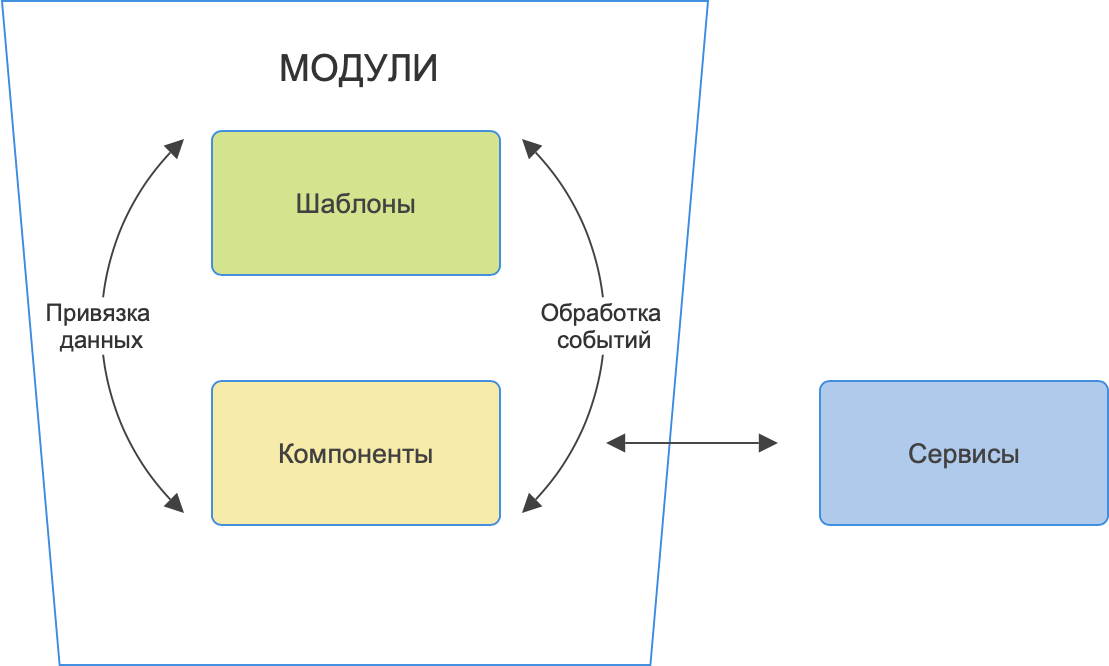
\includegraphics[width=0.8\textwidth]{assets/151}
	\caption*{}
\end{figure}

{\bfseries Рис. 1 - Архитектура Angular}

Архитектура в Angular на Рисунке 1 построена на компонентах, где каждый
компонент включает свою логику, данные и представление. Компоненты
(Component) представляют элементарные части приложения, включающие
HTML-шаблоны, CSS для стилей и TypeScript для логики, позволяя
управление каждой частью, делая их независимыми модулями для реализации
МИС системы. Сервисы (Services) выполняют задачи: получение данных о
пациенте, работа с учетными записями и управление встречами, позволяя
компонентам заниматься на представлении информации пользователя
{[}18{]}.

Модули (Modules) объединяют схожие компоненты и сервисы, предлагая
функции такие, как личная консультация между врачом и пациентом в
отдельный блок. Маршрутизация (Routing) позволяет перемещаться между
страницами приложения, такими как вход, регистрация, просмотр врачей и
запись на прием. Привязка данных (Data binding) и обработка событий
(event handling) автоматически обновляет интерфейс при изменении
состояния приложения. Обработка событий позволяет компонентам
реагировать на действия пациентам, такие как отправка формы заявки или
нажатие кнопки, обеспечивая оперативное взаимодействие {[}18{]}.

Выбранная методология соответствует целям проекта, поскольку направлена
на тщательное исследование, практическую разработку и эффективную
интеграцию функций. Сочетание обзоров литературы и выбранной методологии
обеспечило понимание потребностей пользователей и существующих решений.

{\bfseries Результаты и обсуждение.} Выбор остановился на SQLite для базы
данных из-за её легкости и интеграции с Django фреймворком. SQLite
предлагает простоту и удобство, позволяя сосредоточиться на разработке
без сложной настройки. В дальнейшем система может плавно перейти на
более масштабируемое решение, поддерживаемое Django, благодаря гибкости
SQLite {[}19{]}.

На рисунке 2 представлена схема базы данных (БД) МИС системы. База
данных содержит данные о врачах и пациентах, организуя информацию в
нескольких таблицах. База данных содержит на таблицы, разделенных на три
основные группы (Доктор, Пациент, Запись).

\begin{figure}[H]
	\centering
	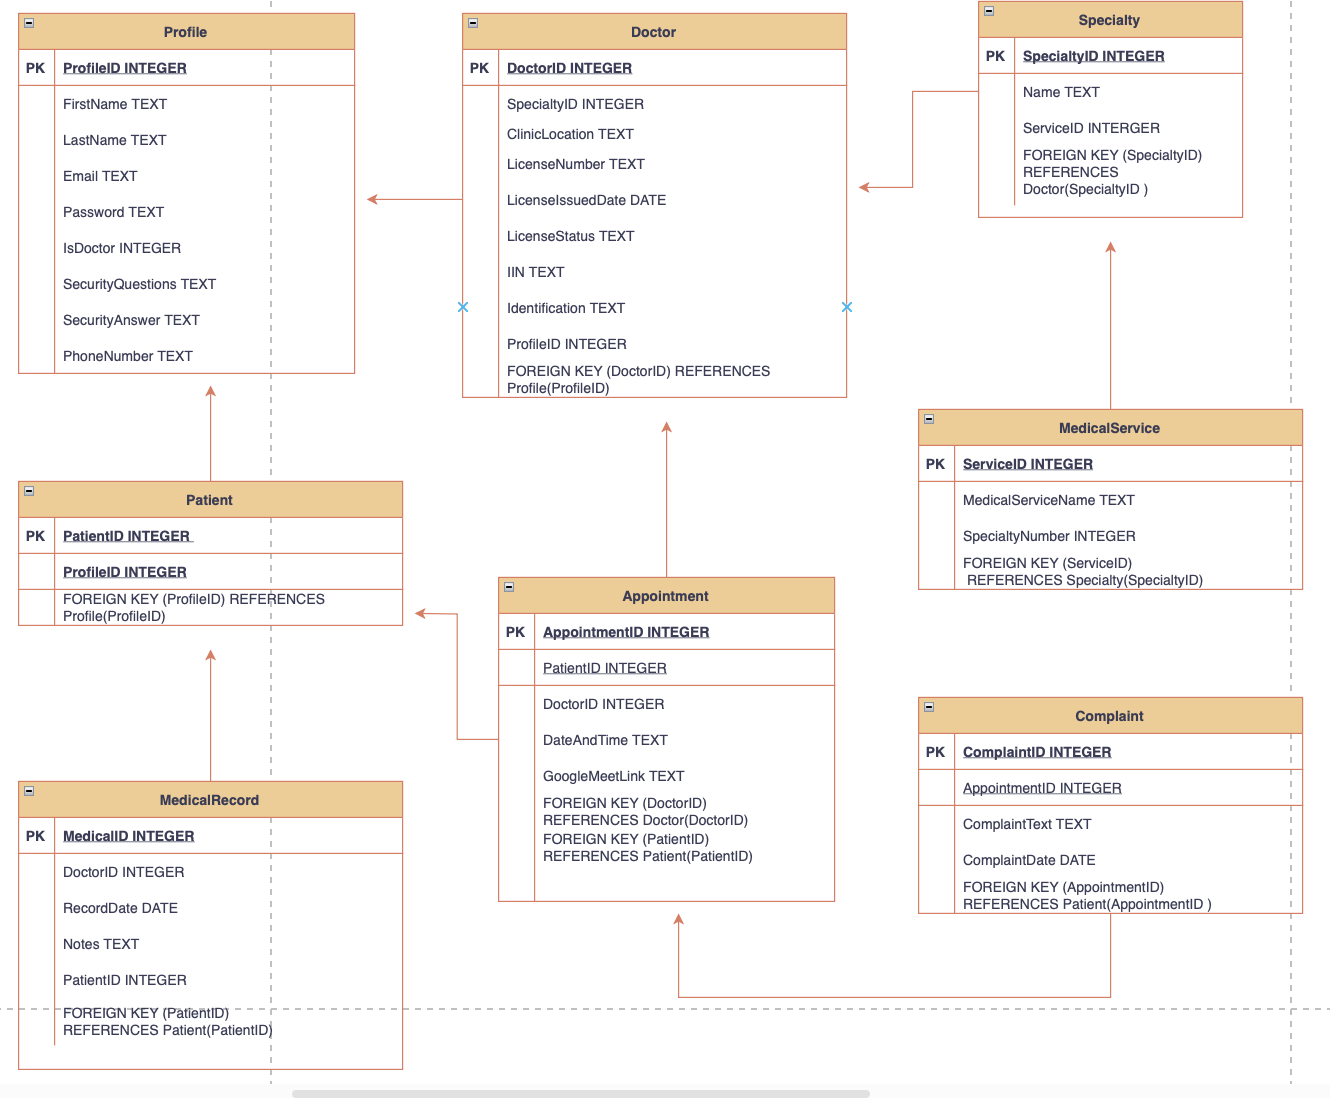
\includegraphics[width=0.8\textwidth]{assets/152}
	\caption*{}
\end{figure}

{\bfseries Рис. 2 -- ERD Диаграмма БД МИС системы}

Профиль (Profile): Содержит основную информацию о пользователе, включая
имя, фамилию, адрес электронной почты, пароль, секретный вопрос и ответ
для верификации, а также индикатор статуса врача.

Доктор (Doctor): Предоставляет дополнительные данные, специфичными для
врачей, такими как специальность, расположение клиники, информация о
лицензии и статус проверки, если профиль является доктором.
Специальность (Specialty): Содержит информацию о врачебных
специальностях. Медицинские услуги (MedicalService) - тождествуется со
соответствующим лечебным специальностям.

Пациент: Расширяет таблицу "Профиль" для представления пациентов, если
запись о профиле является пациентом. Медицинская запись (MedicalRecord):
Сохраняет данные о пациентах.

Запись (Appointment): Управляет деталями встреч между врачами и
пациентами, включая дату, время и ссылку на онлайн-консультации. Жалоба
(Complaint): Обрабатывает жалобы пациентов предварительно до записи на
прием к врачу.

Рисунок 3 показывает структуру нашего бэкенда, организованного по
приложениям:

\begin{figure}[H]
	\centering
	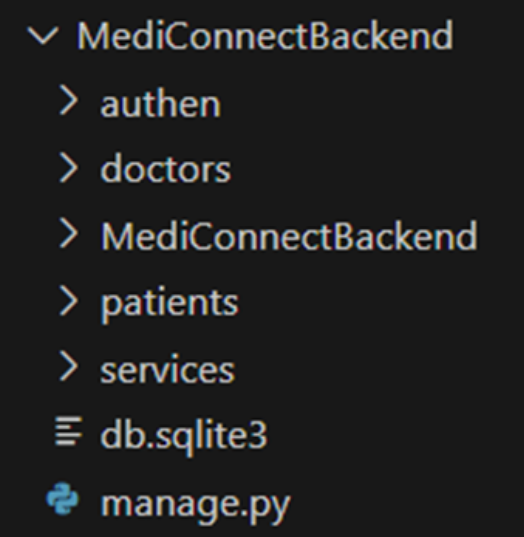
\includegraphics[width=0.8\textwidth]{assets/153}
	\caption*{}
\end{figure}

{\bfseries Рис. 3 - Структура бэкенда системы}

Каждый модуль отвечает со следующие функции:

\begin{enumerate}
\def\labelenumi{\arabic{enumi}.}
\item
  Authen: Аутентификация и управление пользователями.
\item
  Врачи (doctors): Профили врачей, включая специальности и проверку
  лицензий.
\item
  Пациенты (patients): Профили пациентов и их взаимодействие с врачами.
\item
  Услуги (services):Управление медицинскими услугами и запись на прием.
\item
  MediConnectBackend: Основная программа с глобальными настройками и
  конфигурациями.
\end{enumerate}

В проекте запрос поступает к диспетчеру URL-адресов в `urls.py`, который
направляет его к соответствующему представлению в `views.py`.
Представление обрабатывает запрос, проверяет данные, вызывает
бизнес-логику и взаимодействует с моделями из `models.py`, управляющими
базой данных через Django. Для преобразования моделей в JSON и проверки
данных используются сериализаторы из `serializers.py`. После обработки
представление возвращает HTTP-ответ, будь то HTML-шаблон, JSON для API
или перенаправление, указанные на Рисунке 4.

\begin{figure}[H]
	\centering
	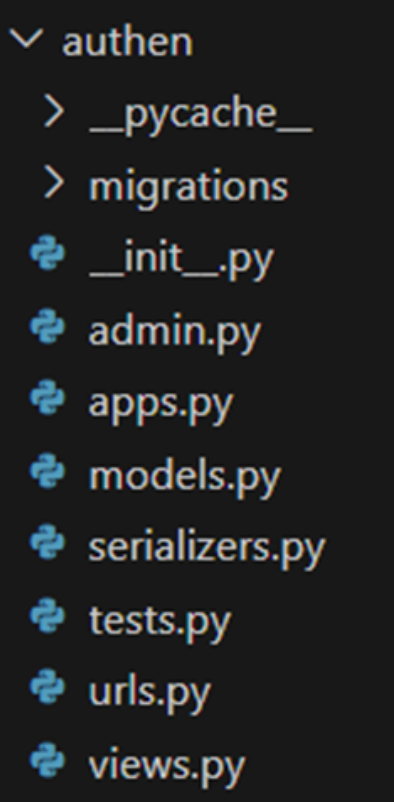
\includegraphics[width=0.8\textwidth]{assets/154}
	\caption*{}
\end{figure}

{\bfseries Рис. 4 - Структура программы}

МИС система обеспечивает доступ к медицинским услугам, позволяя
пользователям искать и планировать встречи. Программа моделируют
специализации, медицинские услуги и посещения, где прием и медицинское
обслуживание соответствуют различным видам услуг. Функциональность,
связанная с доступом к услугам, созданием встреч и изменением данных о
бронировании, реализована в `view.py`.

Дизайн страницы входа позволяет существующим пользователям войти в
систему и обрабатывает данную функциональность, отображен на Рисунке 5.
Пользователям необходимо указать собственный адрес электронной почты и
пароль. Компонент проверяет, заполнены ли оба поля и валидность формата
электронной почты. Если учетные данные верны, пользователь попадает на
домашнюю страницу. Если нет, отображается сообщение об ошибке.

\begin{figure}[H]
	\centering
	
\includegraphics[width=0.8\textwidth]{assets/155}
	\caption*{}
\end{figure}

{\bfseries Рис. 5 - Форма авторизации}

Переходя на страницу выбора определенного доктора, страница сведений о
враче предоставляет подробную информацию, включая его профиль и
назначения, отображен на Рисунке 6. При инициализации компонента данные
о враче извлекаются из параметров маршрута с использованием его
идентификатора. Метод системы получает информацию о профиле врача, такую
как имя, фамилия и адрес электронной почты. Если пользователь не
авторизован, он перенаправляется на страницу входа.

\begin{figure}[H]
	\centering
	
\includegraphics[width=0.8\textwidth]{assets/156}
	\caption*{}
\end{figure}

{\bfseries Рис. 6 - Профиль доктора}

Управление встречами в системы Телемедицины является критическим
элементом, обеспечивающим плавное планирование, наблюдение и
регулирование встреч между врачами и пациентами. Система предоставляет
надежные функции, помогающие упростить все этапы взаимодействия, включая
создание, управление и интеграцию с внешними инструментами. Пользователи
имеют возможность выбирать доступные временные слоты из динамического
календаря, который отображает как свободные, так и зарезервированные
слоты, гарантируя прозрачность и легкость использования системы для
записи на консультацию на Рисунке 7.

\begin{figure}[H]
	\centering
	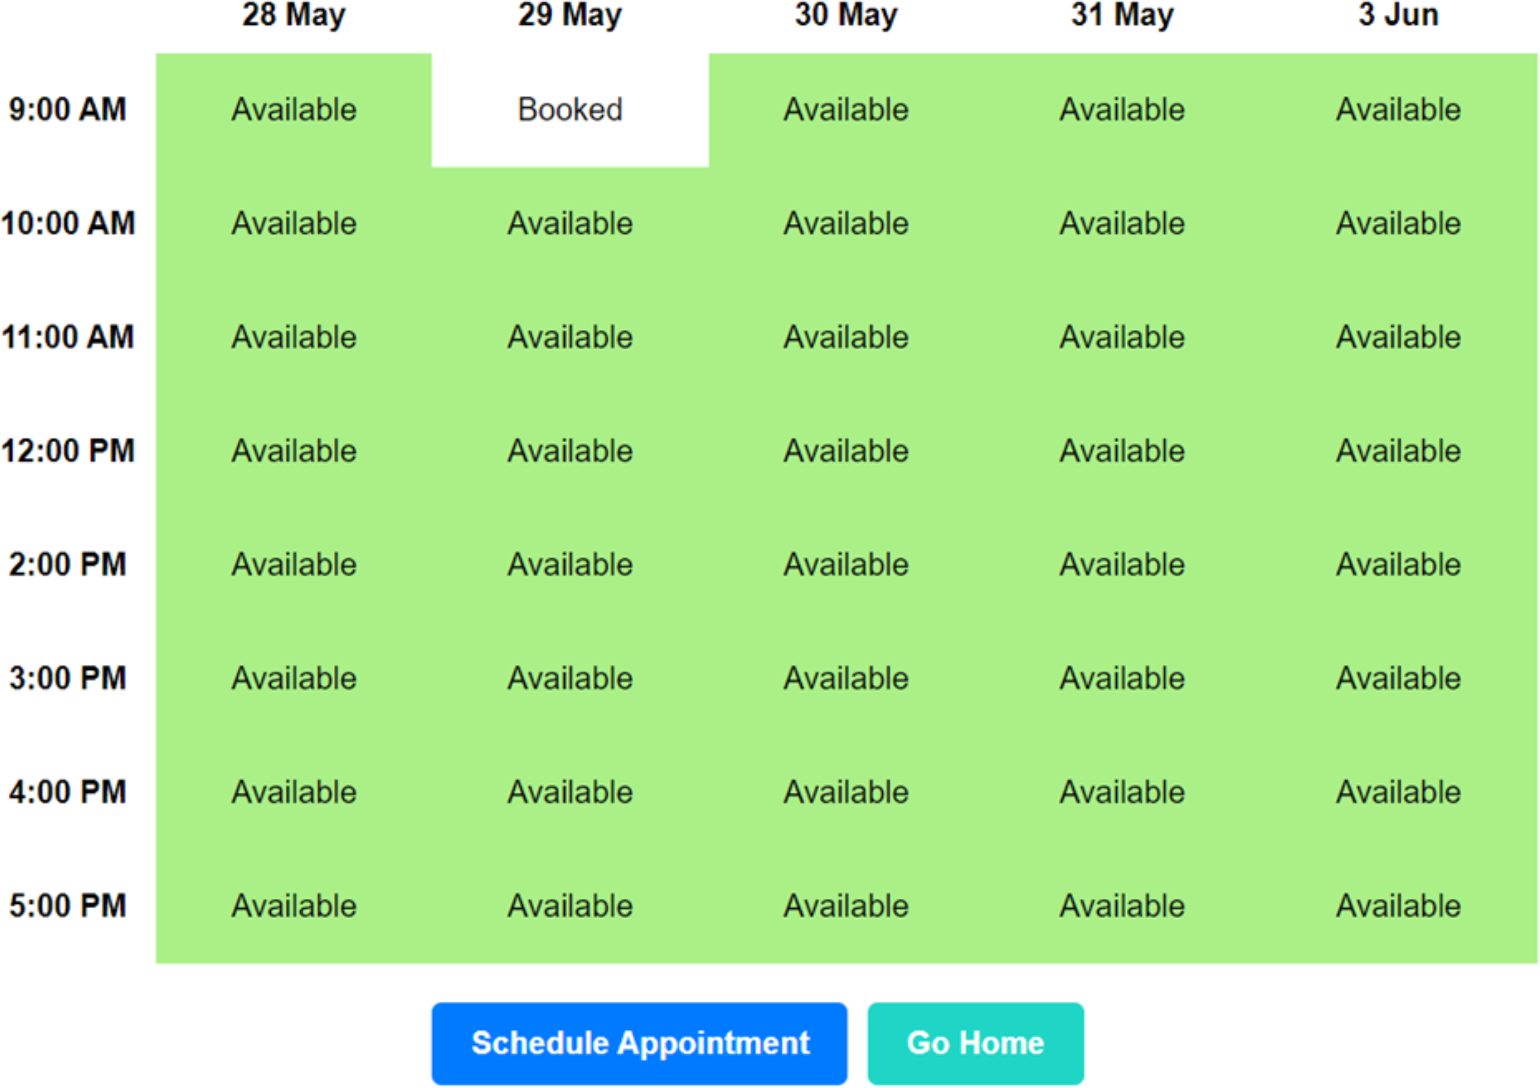
\includegraphics[width=0.8\textwidth]{assets/157}
	\caption*{}
\end{figure}

{\bfseries Рис. 7 - Страница планирования встреч}

Функция планирования встреч в МИС проверяет выбранный интервал и
аутентификацию пользователя. Она извлекает идентификатор пациента и
формирует данные о встрече с использованием идентификатора врача. При
редактировании данные обновляются, при создании встречи они добавляются.
После успешного выполнения операции пользователь получает уведомление, а
при ошибке система предупреждает.

Разработка модели медицинской информационной системы для записи на прием
направлена на облегчение планирования встреч между медицинского
персонала и пациентов. Система обеспечивает удобный интерфейс для записи
на прием к врачу, управления расписанием и проведения медицинских
консультаций.

Для непрерывного улучшения системы существенно необходимо собирать
обратную связь от пользователей через опросы, фокус-группы или
индивидуальные интервью. Это позволит оценить их опыт, выявить узкие
места и определить приоритеты для будущих улучшений. Такой подход
приводит к повышению эффективности работы системы, улучшению качества
заботы о пациентах и обеспечивает бесперебойное функционирование.

{\bfseries Выводы.} В результате проведенного исследования была разработана
и предложена модель медицинской информационной системы (МИС) для
телемедицины, ориентированная на улучшение процесса записи пациентов к
медицинским специалистам. Основной целью данной работы было создание
решения, направленного на повышение качества медицинских услуг,
оптимизацию административных процессов и расширение доступа к
медицинским услугам для пациентов, особенно в удаленных регионах.

Для разработки системы использовались современные веб-технологии: Django
для серверной части, Angular для внешнего интерфейса и SQLite для
управления базами данных. Основные модули системы включают регистрацию и
аутентификацию пользователей, управление профилями пациентов и врачей, а
также планирование встреч.

Анализ производительности системы показал, что использование базы данных
SQLite позволяет эффективно обрабатывать записи пациентов и медицинских
специалистов. Однако SQLite ограничивает масштабируемость системы. Для
крупных медицинских учреждений с большим объемом данных и пользователей
необходимо перейти на более мощные системы управления базами данных.

Качественные показатели работы системы показывают, что улучшено
взаимодействие между пациентами и медицинским персоналом, а также
упрощен процесс записи. Однако текущая версия системы требует
дополнительных мер для усиления безопасности данных, что особенно важно
при работе с конфиденциальной медицинской информацией. Требуется
внедрение улучшенных механизмов аутентификации и верификации.

Система прошла апробацию медицинскими специалистами клиники «Aisera
Clinic» в городе Астана, где продемонстрировала свою эффективность и
надежность. Результаты апробации подтверждают, что внедрение МИС
способствует упрощению процессов записи и обработки информации о
пациентах, а также улучшению качества предоставляемых медицинских услуг.

В дальнейшем развитии системы планируется интеграция дополнительных
функций, усиление мер безопасности и улучшение пользовательского
интерфейса для более эффективного обслуживания пользователей и обработки
больших объемов данных. Также предусмотрено расширение системы для
крупных учреждений с применением более мощных баз данных и улучшенной
системы безопасности.

Таким образом, разработанная медицинская информационная система
представляет значительный прогресс в управлении медицинскими услугами,
предоставляя комплексное решение для записи на прием и
онлайн-консультаций. С постоянным развитием и адаптацией к изменяющимся
потребностям, МИС будет продолжать обеспечивать высокий уровень
эффективности и доступности медицинских услуг в условиях цифровой
трансформации здравоохранения.

{\bfseries Литература}

\begin{enumerate}
\def\labelenumi{\arabic{enumi}.}
\item
  Giansanti D. Ten years of telehealth and digital healthcare: Where are
  we? //Healthcare. -- MDPI.- 2023. - Vol. 11. -- №. 6. DOI
  10.3390/healthcare11060875
\item
  Smith A. C., Thomas E., Snoswell C. L., Haydon H., Mehrotra A.,
  Clemensen J., and Caffery L.J. Telehealth for global emergencies:
  Implications for coronavirus disease 2019 (COVID-19) //Journal of
  telemedicine and telecare.- -2020.-Vol.26(5).- P. 309-313.
\end{enumerate}

DOI 10.1177/1357633X20916567

\begin{enumerate}
\def\labelenumi{\arabic{enumi}.}
\setcounter{enumi}{2}
\item
  Betancourt J. A., Rosenberg M. A., Zevallos A., Brown J. R., and
  Mileski M. The impact of COVID-19 on telemedicine utilization across
  multiple service lines in the United States //Healthcare. -- MDPI.-
  2020. -Vol. 8(4). DOI 10.3390/healthcare8040380
\item
  Alotaibi Y. K., Federico F. The impact of health information
  technology on patient safety //Saudi medical journal. - 2017. -Vol.
  38(12). - P. 1173-1180. DOI 10.15537/smj.2017.12.20631
\item
  Phuong J., Ordóñez P., Cao J., Moukheiber M., Moukheiber L., Caspi A.,
  and Mankoff J. Telehealth and digital health innovations: A mixed
  landscape of access //PLOS Digital Health. -- 2023. - Vol. 2(12). DOI
  10.1371/journal.pdig.0000401
\item
  Ma Y., Zhao C., Zhao Y., Lu J., Jiang H., Cao Y., and Xu Y.
  Telemedicine application in patients with chronic disease: a
  systematic review and meta-analysis //BMC medical informatics and
  decision making. - 2022. -Vol. 22(1). DOI 10.1186/s12911-022-01845-2.
\item
  Seitenov A., Zhukabayeva T., Sansyzbay K., Kalpakov E. Design
  development of medicine information system for telemedicine field
  //The Bulletin of KazATC.- 2023. -Vol. 127(4).- P. 241-251. DOI
  10.52167/1609-1817-2023-127-4-241-251
\end{enumerate}

Akhtar M. N., Haleem A., Javaid M. Scope of health care system in rural
areas under Medical 4.0 environment //Intelligent Pharmacy.- 2023. -Vol.
1(4). - P. 217-223.

DOI 10.1016/j.ipha.2023.07.003

\begin{enumerate}
\def\labelenumi{\arabic{enumi}.}
\setcounter{enumi}{7}
\item
  Kim Y.S. Telemedicine in the USA with focus on clinical applications
  and issues //Yonsei medical journal. -2004.- Vol. 45(5).- P. 761-775.
  DOI 10.3349/ymj.2004.45.5.761
\item
  Shen Y.T., Che L., Yue W.W., and Xu H.X. Digital technology-based
  telemedicine for the COVID-19 pandemic //Frontiers in medicine. -
  2021.-Vol. 8. DOI 10.3389/fmed.2021.646506
\item
  Epizitone A., Moyane S.P., Agbehadji I.E. A systematic literature
  review of health information systems for healthcare //Healthcare.-
  MDPI.-2023.-Vol. 11(7).
\end{enumerate}

DOI 10.3390/healthcare11070959

\begin{enumerate}
\def\labelenumi{\arabic{enumi}.}
\setcounter{enumi}{10}
\item
  Palozzi G., Schettini I., Chirico A. Enhancing the sustainable goal of
  access to healthcare: findings from a literature review on
  telemedicine employment in rural areas //Sustainability. -- 2020. -
  Vol. 12(8). DOI 10.3390/su12083318
\item
  Combi C., Pozzani G., Pozzi G. Telemedicine for developing countries.
  A Survey and Some Design Issues //Applied Clinical Informatics.-2016.
  -Vol. 7(4). - P. 1025-1050.
\end{enumerate}

DOI 10.4338/ACI-2016-06-R-0089

\begin{enumerate}
\def\labelenumi{\arabic{enumi}.}
\setcounter{enumi}{12}
\item
  Shigekawa E., Fix M., Corbett G., Roby D. H., and Coffman, J. The
  current state of telehealth evidence: a rapid review //Health
  Affairs.-2018. --Vol. 37(12) -P. 1975-1982.
\end{enumerate}

DOI 10.1377/hlthaff.2018.05132

\begin{enumerate}
\def\labelenumi{\arabic{enumi}.}
\setcounter{enumi}{13}
\item
  Dullet N.W. Geraghty E.M., Kaufman T., Kissee J.L., King J., Dharmar
  M., and Marcin J.P. Impact of a university-based outpatient
  telemedicine program on time savings, travel costs, and environmental
  pollutants //Value in Health. -- 2017. -- Vol. 20(4). -- P. 542-546.
  DOI 10.1016/j.jval.2017.01.014
\item
  De La Torre-Díez I. López-Coronado M., Vaca C., Aguado J. S., and de
  la Torre B. Cost-utility and cost-effectiveness studies of
  telemedicine, electronic, and mobile health systems in the literature:
  a systematic review //Telemedicine and e-Health. -2015.-Vol. 21(2).
  -P. 81-85.
\end{enumerate}

DOI 10.1089/tmj.2014.0053

\begin{enumerate}
\def\labelenumi{\arabic{enumi}.}
\setcounter{enumi}{15}
\item
  Agarwal S., LeFevre A. E., Lee J., L'engle K., Mehl G., Sinha C., \&
  Labrique, A. Guidelines for reporting of health interventions using
  mobile phones: mobile health (mHealth) evidence reporting and
  assessment (mERA) checklist. //bmj. - 2016. -Vol. 352. DOI
  10.1136/bmj.i1174
\item
  Garg, A. What is Angular?: Syntax, Features, Architecture, \& More:
  Internshala Trainings Blog. - URL:
  https://trainings.internshala.com/blog/what-is-angular/
\item
  Priy S. Introduction to SQLite. // GeeksforGeeks.
\end{enumerate}

URL: https://www.geeksforgeeks.org/introduction-to-sqlite/

\emph{{\bfseries Сведения об авторах}}

Сейтенов А.С. - докторант, Евразийский национальный университет им. Л.
Н. Гумилева, Астана, Казахстан, e-mail: altynbekss@gmail.com;

Жукабаева Т.К. - PhD, профессор Евразийский национальный университет им.
Л. Н. Гумилева, Астана, Казахстан,e-mail: tamara.kokenovna@gmail.com;

Al-Majeed S. - PhD, профессор, Al Akhawayn University, Ифран, Марокко,
e-mail: salah.almajeed@gmail.com;

Wolff C. - PhD, профессор, Fachhochschule Dortmund, Дортмунд,
Германия,,e-mail: carsten.wolff@fh-dortmund.de

\emph{{\bfseries Information about the authors}}

Seitenov A.S. - PhD student, L.N.Gumilyov Eurasian National University,
Astana, Kazakhstan, e-mail: altynbekss@gmail.com;

Zhukabayeva T.K. - PhD, professor, L.N.Gumilyov Eurasian National
University, Astana, Kazakhstan, e-mail: tamara.kokenovna@gmail.com;

Al-Majeed S. - PhD, professor, Al Akhawayn University, Ifrane, Morocco,
e-mail: salah.almajeed@gmail.com;

Wolff C. - PhD, professor, Fachhochschule Dortmund, Dortmund, Germany,
e-mail: carsten.wolff@fh-dortmund.de